%%% main.tex — SF6 ICP Etch Surrogate Model Report
%%% Reframed: new work since last meeting (solver already known)
\documentclass[12pt,a4paper]{article}

% ---------- packages ----------
\usepackage[margin=1in]{geometry}
\usepackage{amsmath,amssymb}
\usepackage{booktabs}
\usepackage{graphicx}
\usepackage[colorlinks=true,linkcolor=blue,citecolor=blue,urlcolor=blue]{hyperref}
\usepackage{siunitx}
\usepackage[round]{natbib}
\usepackage{float}
\usepackage{caption}
\usepackage{subcaption}

\graphicspath{{../figures/}}
\tolerance=1000
\emergencystretch=1em

\sisetup{
  separate-uncertainty = true,
  multi-part-units     = single,
}

\title{%
  From Fluid Solver to Production Surrogate:\\
  PINN Failure, Supervised Learning Success,
  and LXCat Cross-Section Insights\\
  for SF\textsubscript{6}/Ar ICP Etch Modelling}

\author{%
  Z.\ Ngan \\
  \textit{ngankait@gmail.com}}

\date{April 2026}

% ------------------------------------------------------------------
\begin{document}
\maketitle

% ==================================================================
\begin{abstract}
Starting from the validated 2D axisymmetric fluid solver for a TEL
SF\textsubscript{6}/Ar inductively coupled plasma (ICP) etcher, we
report three lines of investigation pursued since the last meeting.
First, a physics-informed neural network (PINN) approach was attempted
and failed: PDE-constrained training diverges due to five interacting
root causes, while data-only training converges readily
($23{,}000\times$ loss reduction), motivating a pivot to supervised
surrogates.  Second, a systematic surrogate development progressed
through four generations---v1 (nF RMSE 0.133), v2 (0.111), v3
(0.023), v4 (0.003)---via data enrichment, physics regularisation, and
ensemble uncertainty quantification, achieving a $531\times$ speedup
over the legacy solver.  Third, integration of LXCat/Biagi
cross-section data revealed that the electron temperature increases by
56\% and electron density decreases by 69\%, while F density is
unchanged.  A controlled architecture sweep (7 experiments, 3 seeds
each) identified the E3\_separate\_heads topology as the winner, and a
5-model production ensemble achieves nF RMSE $= 0.00154$ and
nSF\textsubscript{6} RMSE $= 0.00128$---a 47\% improvement over the
legacy v4 surrogate.  Ablation reveals output-bias initialisation as
the dominant factor (83\% of RMSE reduction).  The surrogate delivers
an $874\times$ speedup over the LXCat solver.  Limitations are
discussed candidly, including a 36\% systematic error in absolute F
density versus published measurements.
\end{abstract}

\newpage
\tableofcontents
\newpage

% ==================================================================
\section{Introduction}
\label{sec:intro}

In our last meeting we reviewed the two-dimensional axisymmetric fluid
solver for a TEL inductively coupled plasma (ICP) etcher operating in
SF\textsubscript{6}/Ar mixtures.  That solver---with its 54-reaction
Arrhenius chemistry set~\citep{lallement2009}, drift--diffusion
transport, and Robin boundary conditions---is now the established
baseline.  This report covers everything accomplished since then.

Three directions were pursued:
\begin{enumerate}
  \item \textbf{PINN for spatial acceleration
        (Section~\ref{sec:pinn}):} We attempted to embed the governing
        PDEs directly into the neural-network loss function.  This
        failed due to stiff chemistry, cylindrical singularities, and
        multi-scale loss competition.  The negative result is
        documented with a five-point root-cause analysis.
  \item \textbf{Supervised surrogate development
        (Sections~\ref{sec:surrogate}--\ref{sec:production}):}
        Pivoting from PINNs, we built a feedforward surrogate that
        progressed through four generations (v1--v4) and then underwent
        a controlled architecture sweep, ablation study, and ensemble
        optimisation to reach production quality.
  \item \textbf{LXCat physics upgrade
        (Section~\ref{sec:lxcat}):} Biagi cross sections were
        integrated into the solver.  The physics impact was dramatic
        ($T_e$ +56\%, $n_e$ $-$69\%, F unchanged), but a dataset
        diagnosis revealed that the 3.85$\times$ RMSE gap between
        legacy and LXCat surrogates was caused by the training recipe,
        not physics difficulty.
\end{enumerate}

The report is structured to follow this narrative arc:
Sections~\ref{sec:recap}--\ref{sec:sim_recap} briefly recap the
solver (already reviewed); Section~\ref{sec:pinn} documents the PINN
failure; Sections~\ref{sec:surrogate}--\ref{sec:production} present
the surrogate development; Section~\ref{sec:lxcat} covers the LXCat
integration; Sections~\ref{sec:arch_sweep}--\ref{sec:ablation}
describe the architecture search and ablation;
Section~\ref{sec:validation} presents validation;
Section~\ref{sec:supplementary} reports supplementary experiments; and
Sections~\ref{sec:discussion}--\ref{sec:conclusion} discuss findings
and conclude.

% ==================================================================
\section{Solver Recap}
\label{sec:recap}

This section provides a brief summary of the 2D TEL fluid solver for
readers' convenience; full details were presented at the last meeting.

\subsection{Geometry and Governing Equations}

The reactor is a TEL ICP etcher with a T-shaped axisymmetric geometry
comprising an ICP source ($R = \SI{38}{\milli\metre}$,
$L = \SI{181.5}{\milli\metre}$), a \SI{2}{\milli\metre} aperture, and
a processing chamber ($R = \SI{105}{\milli\metre}$,
$L = \SI{50}{\milli\metre}$) where the wafer sits
(Figure~\ref{fig:geom_pair}).  The solver discretises continuity
equations for each species on a structured $(r, z)$ mesh with
drift--diffusion transport, Robin boundary conditions at material
walls~\citep{kokkoris2008}, and the 54-reaction Arrhenius chemistry
set of \citet{lallement2009}.  An electron energy equation provides
$T_e$.

\begin{figure}[H]
  \centering
  \begin{subfigure}[t]{0.48\textwidth}
    \centering
    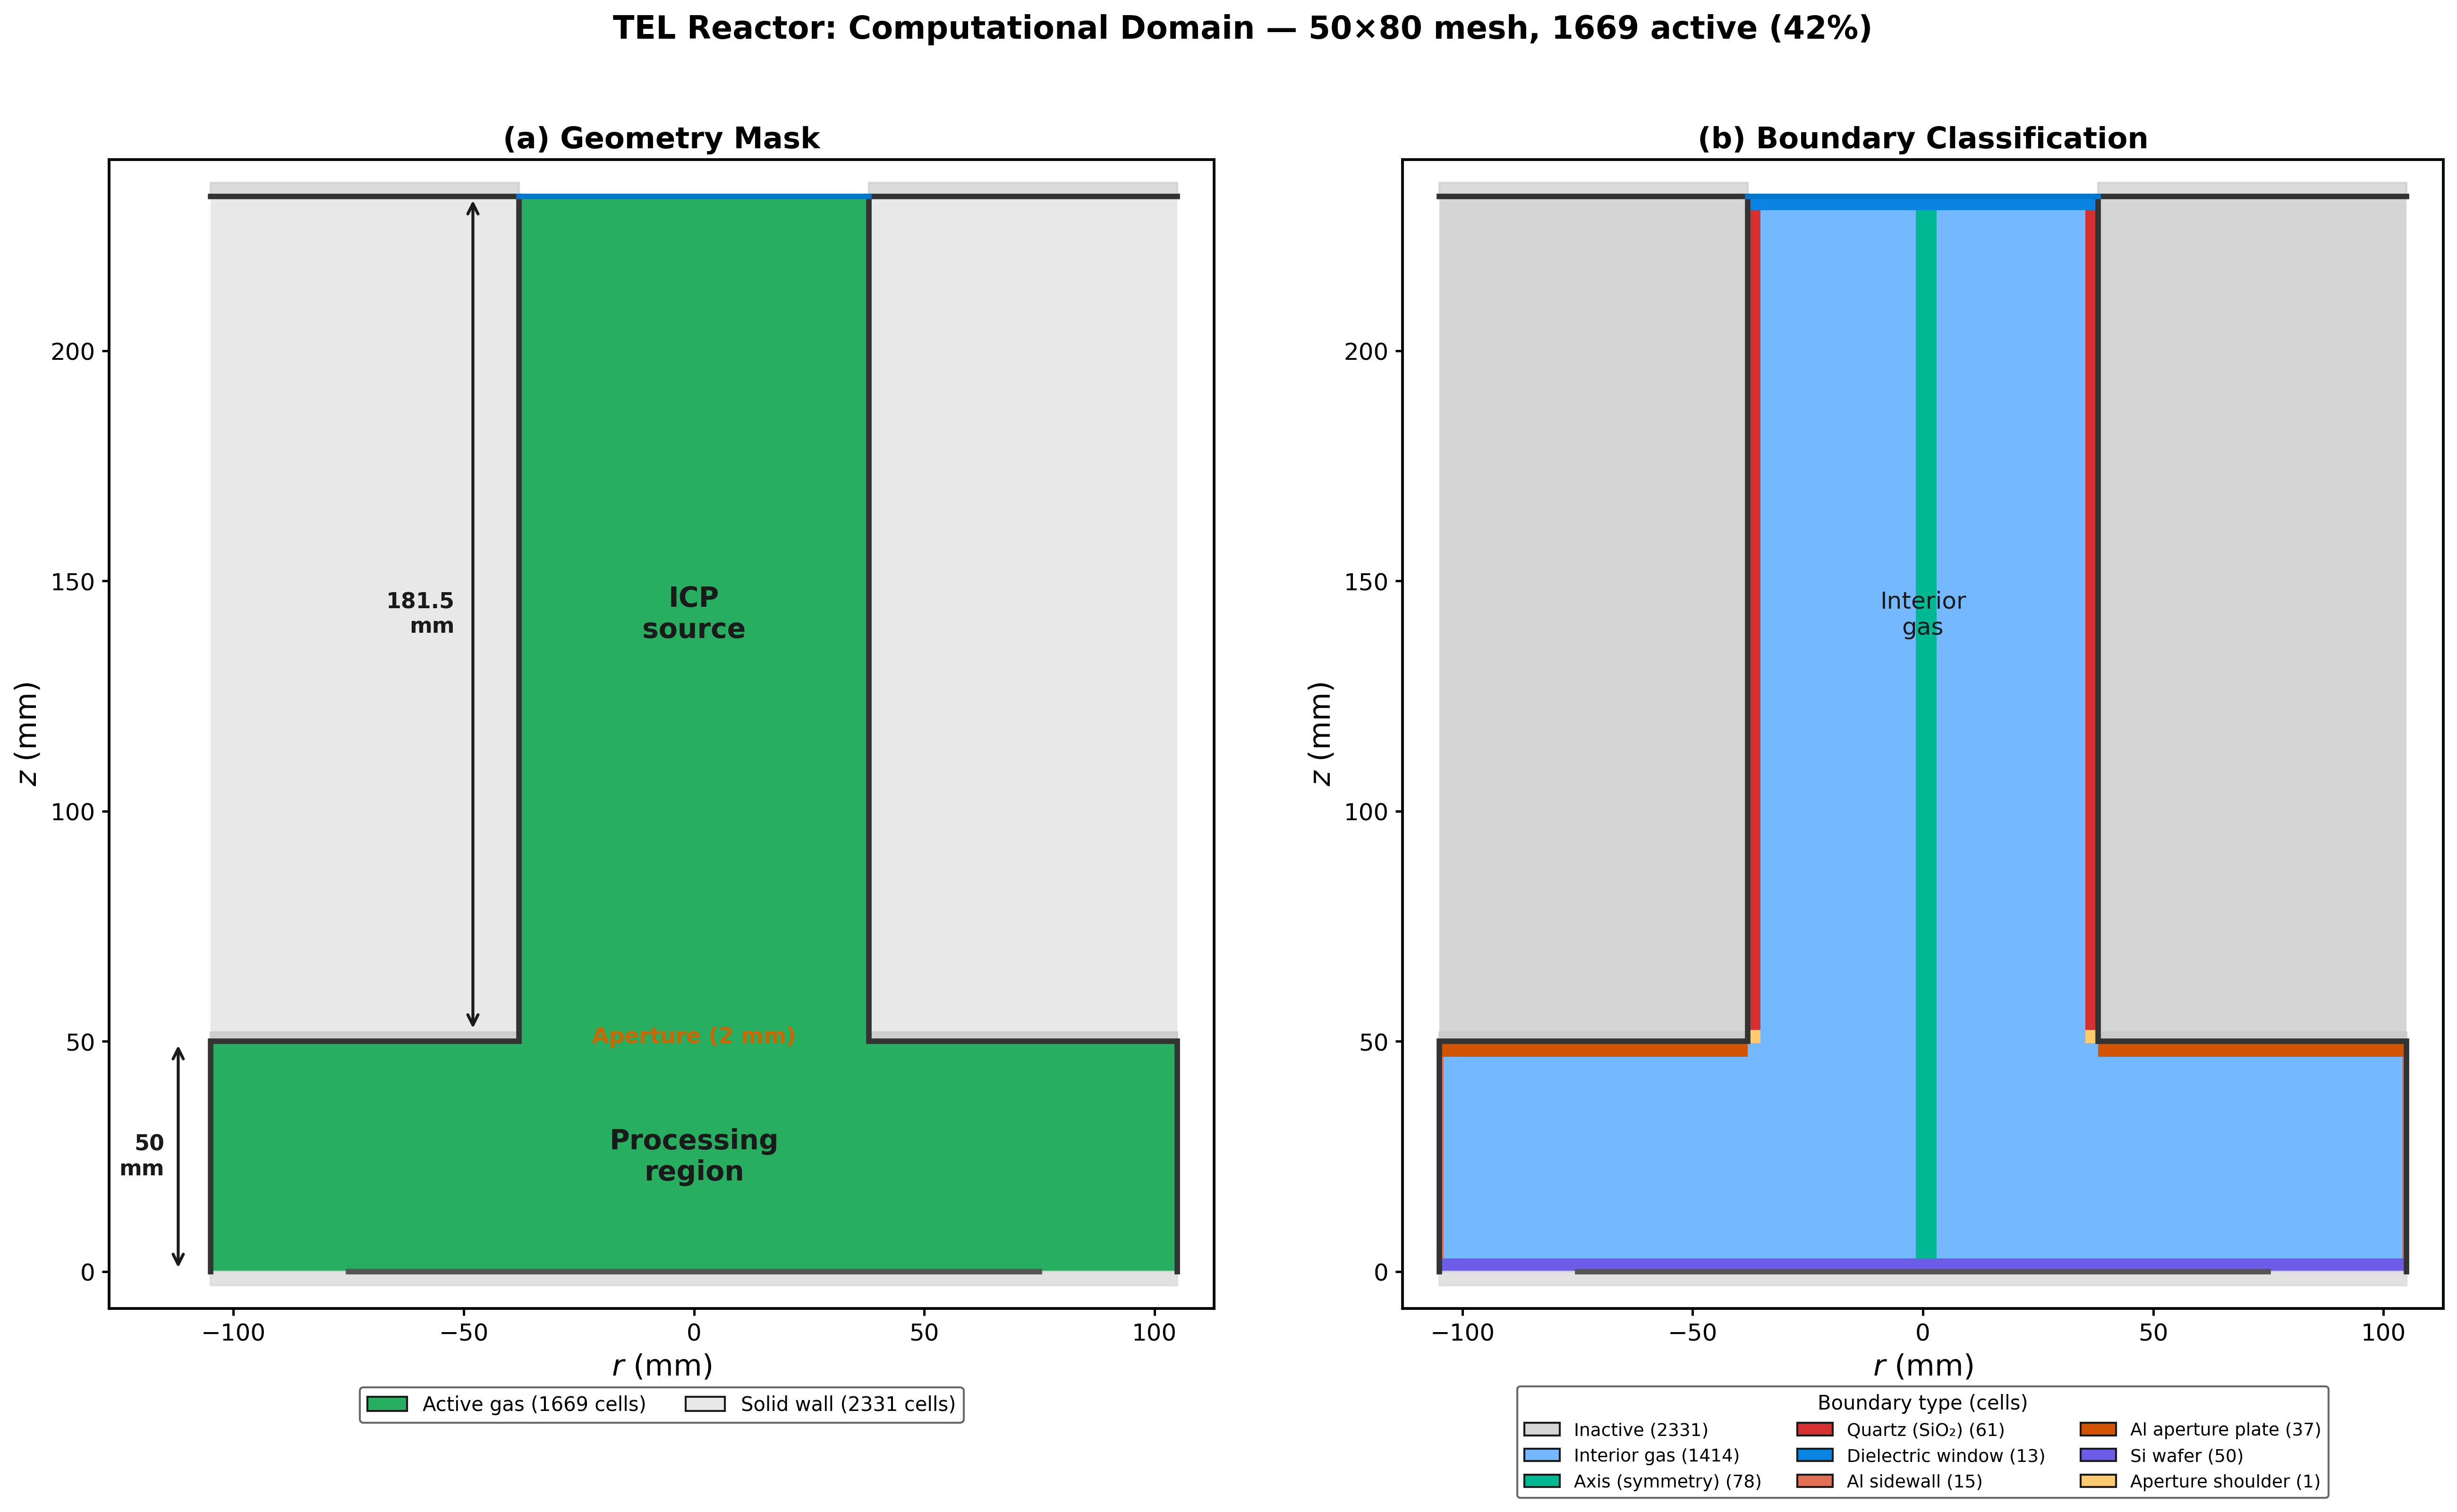
\includegraphics[width=\textwidth]{geometry_mask.png}
    \caption{Full reactor geometry showing the ICP source,
             aperture, and processing regions with the
             computational mask.}
    \label{fig:geometry}
  \end{subfigure}
  \hfill
  \begin{subfigure}[t]{0.48\textwidth}
    \centering
    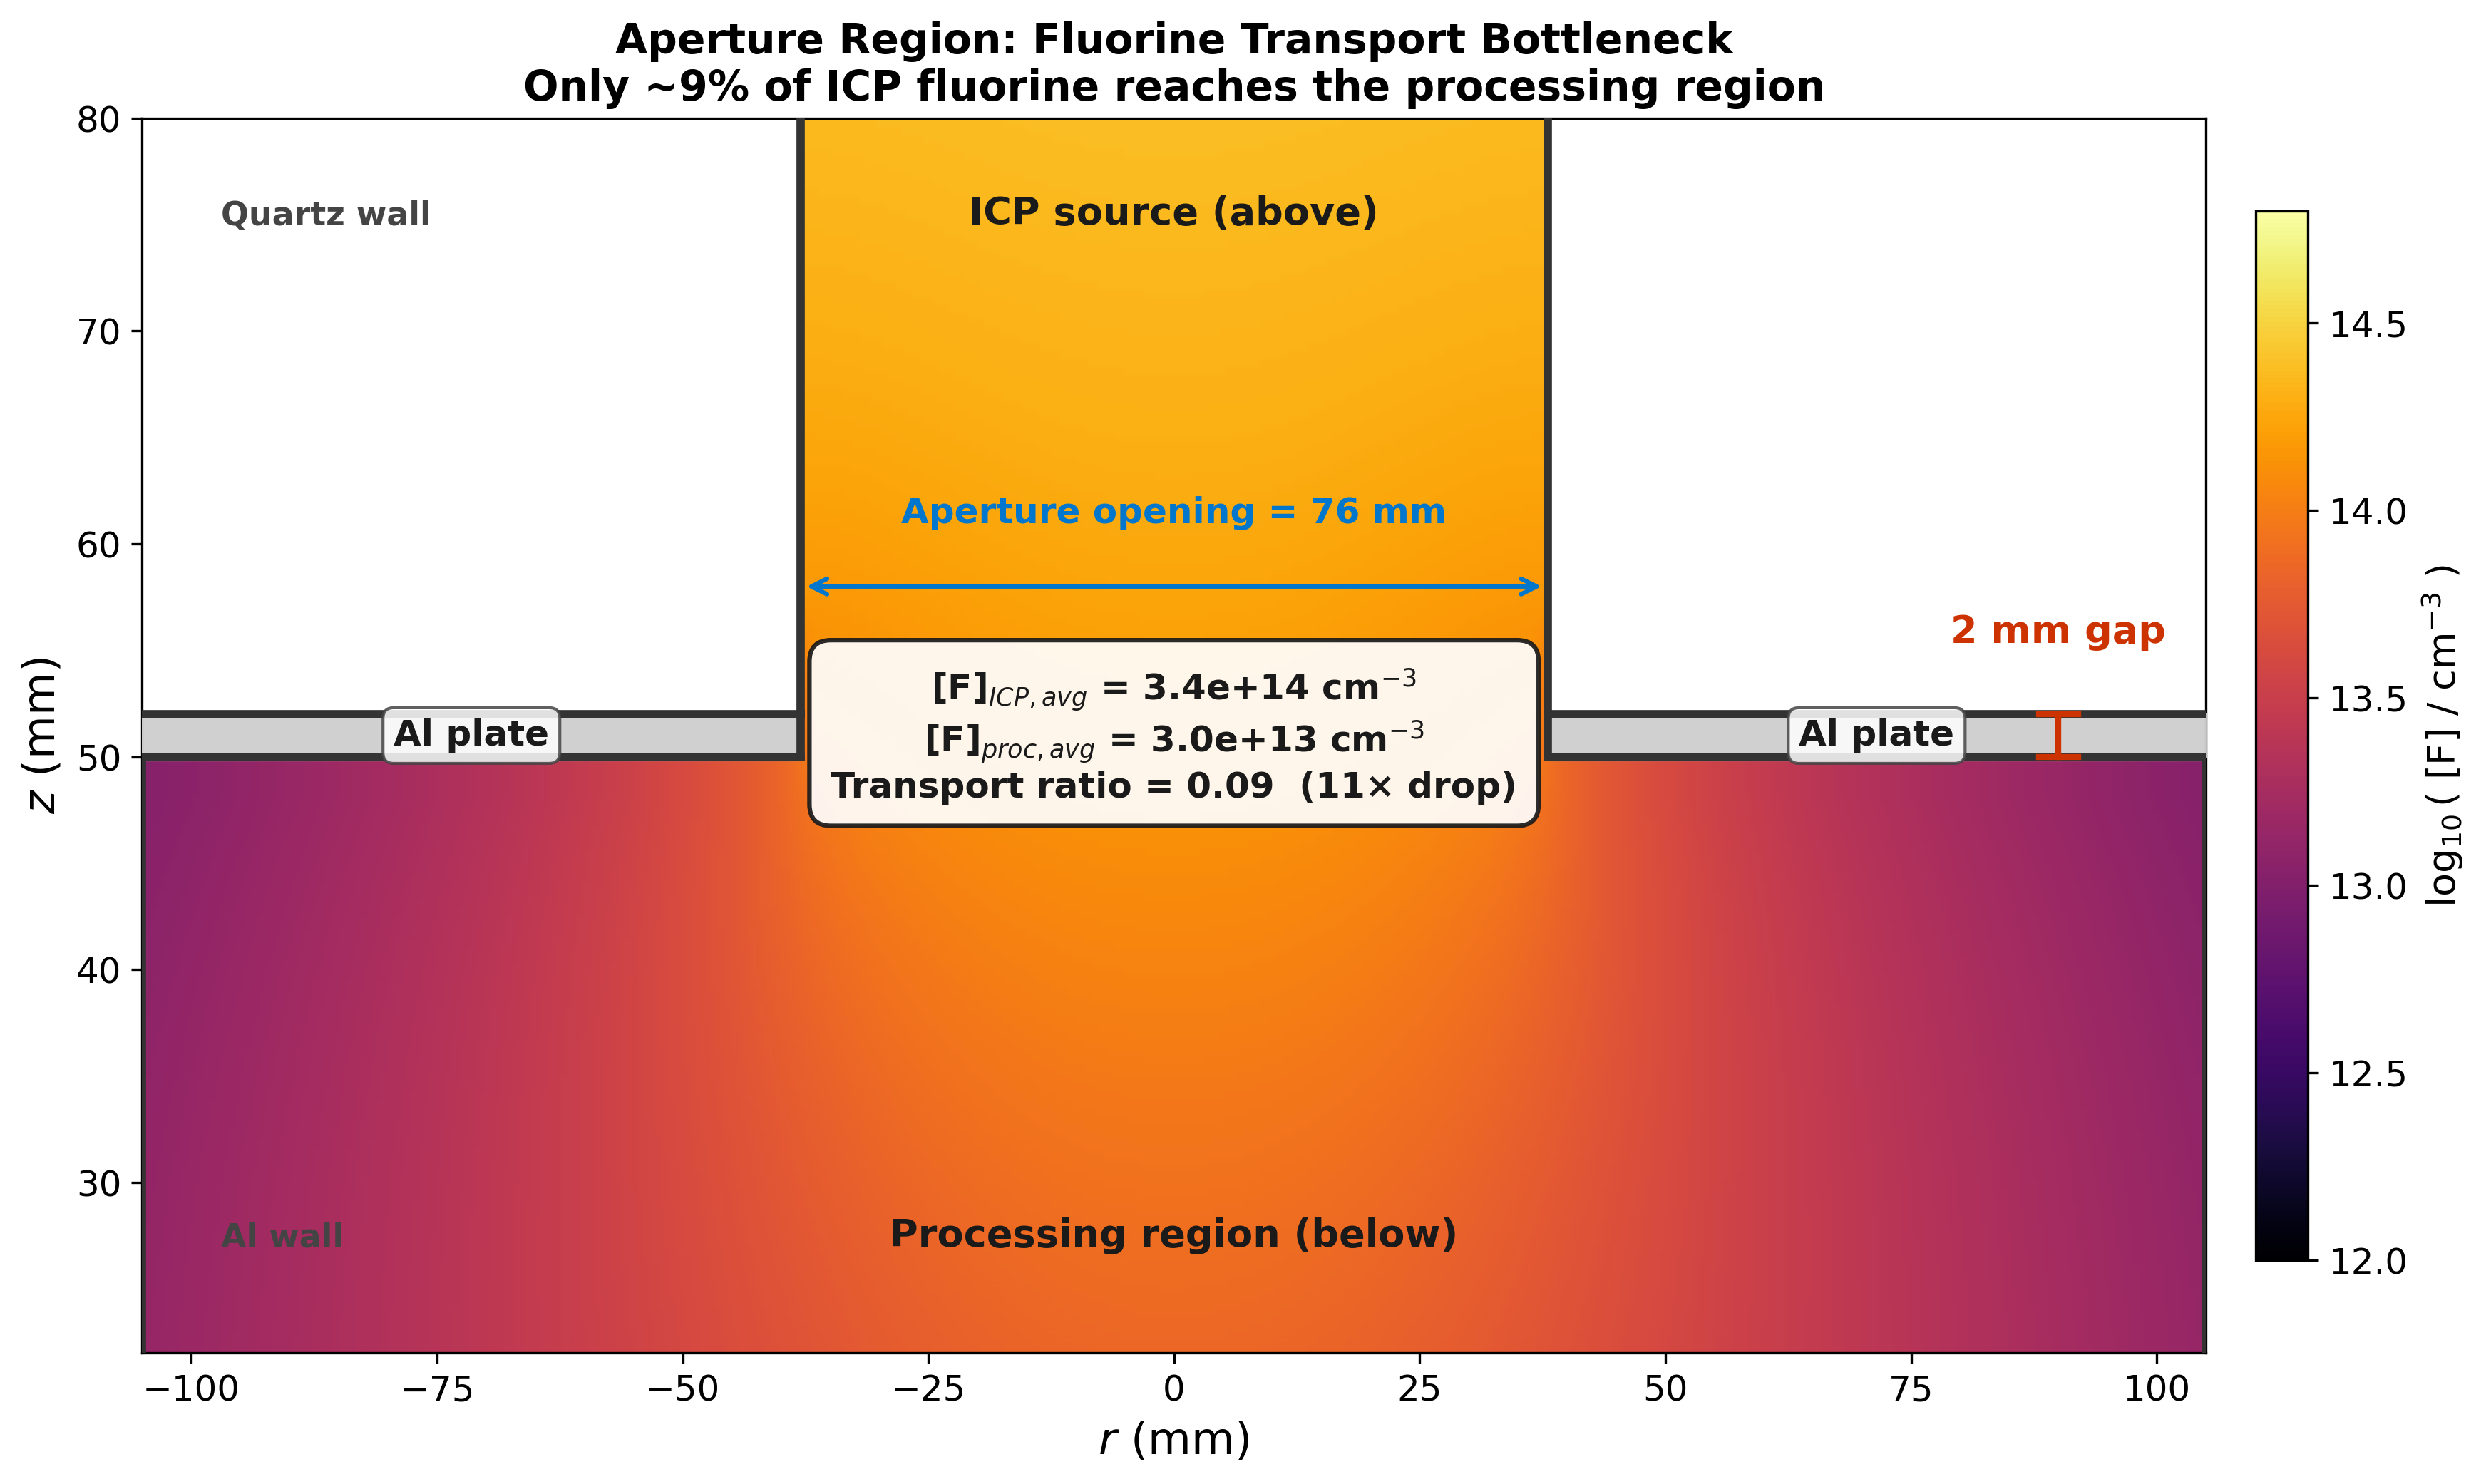
\includegraphics[width=\textwidth]{aperture_zoom.png}
    \caption{Zoomed view of the aperture region connecting the
             ICP source to the processing chamber.}
    \label{fig:aperture}
  \end{subfigure}
  \caption{Reactor geometry.  The T-shaped domain is solved in 2D
           axisymmetric cylindrical coordinates.}
  \label{fig:geom_pair}
\end{figure}

\subsection{Solver Performance and Operating Ranges}

The legacy solver (tabulated cross sections) requires
\SI{7.76}{\second} per operating-point evaluation; the LXCat solver
increases this to \SI{14.4}{\second}.  The operating-parameter space
spans $P_{\text{rf}} \in [200, 1200]\;\si{\watt}$,
$p \in [3, 20]$~mTorr, and $x_{\text{Ar}} \in [0, 50]\%$.
Figure~\ref{fig:em_power} shows the electromagnetic power deposition
profile that drives the discharge.

\begin{figure}[H]
  \centering
  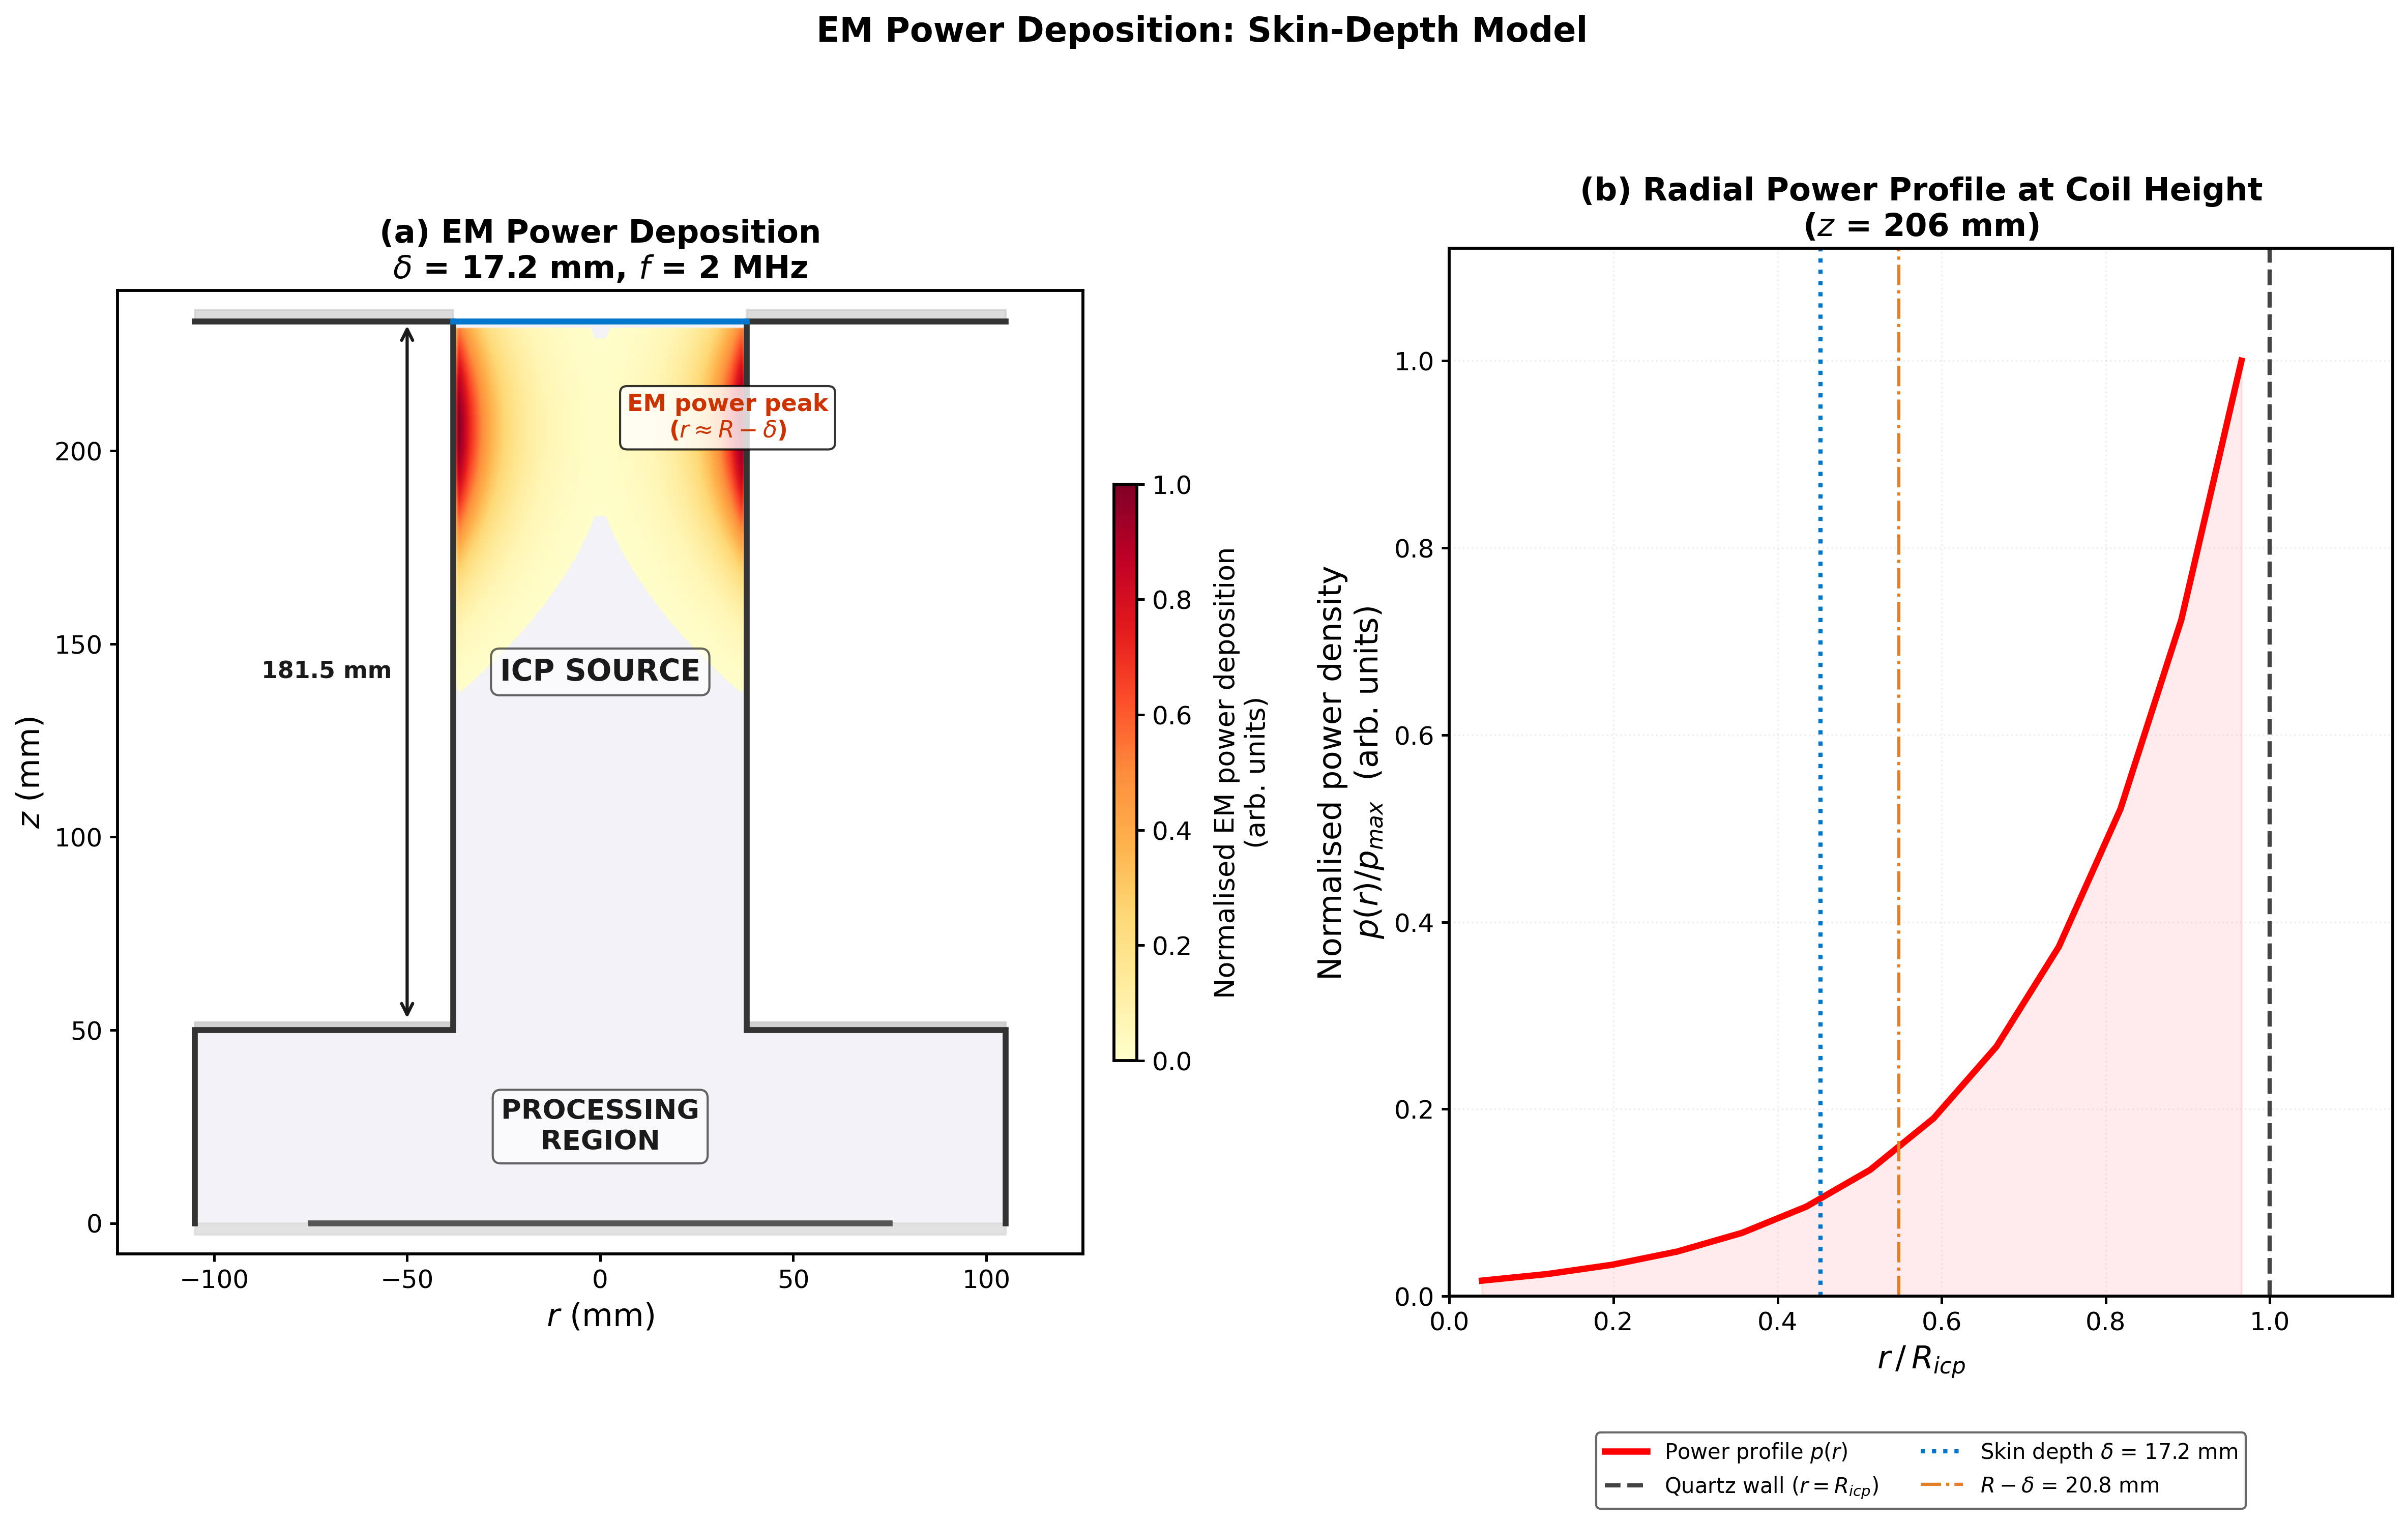
\includegraphics[width=0.55\textwidth]{em_power_deposition.png}
  \caption{Electromagnetic power deposition profile in the ICP
           source region.  Power is concentrated near the coil
           windings and decays exponentially with the skin depth.}
  \label{fig:em_power}
\end{figure}

% ==================================================================
\section{Representative Solver Output}
\label{sec:sim_recap}

Before turning to the new work, we show representative solver outputs
to establish the physical phenomena the surrogate must capture.
Figures~\ref{fig:contours}--\ref{fig:bars} illustrate the spatial and
compositional structure of the discharge.

\begin{figure}[H]
  \centering
  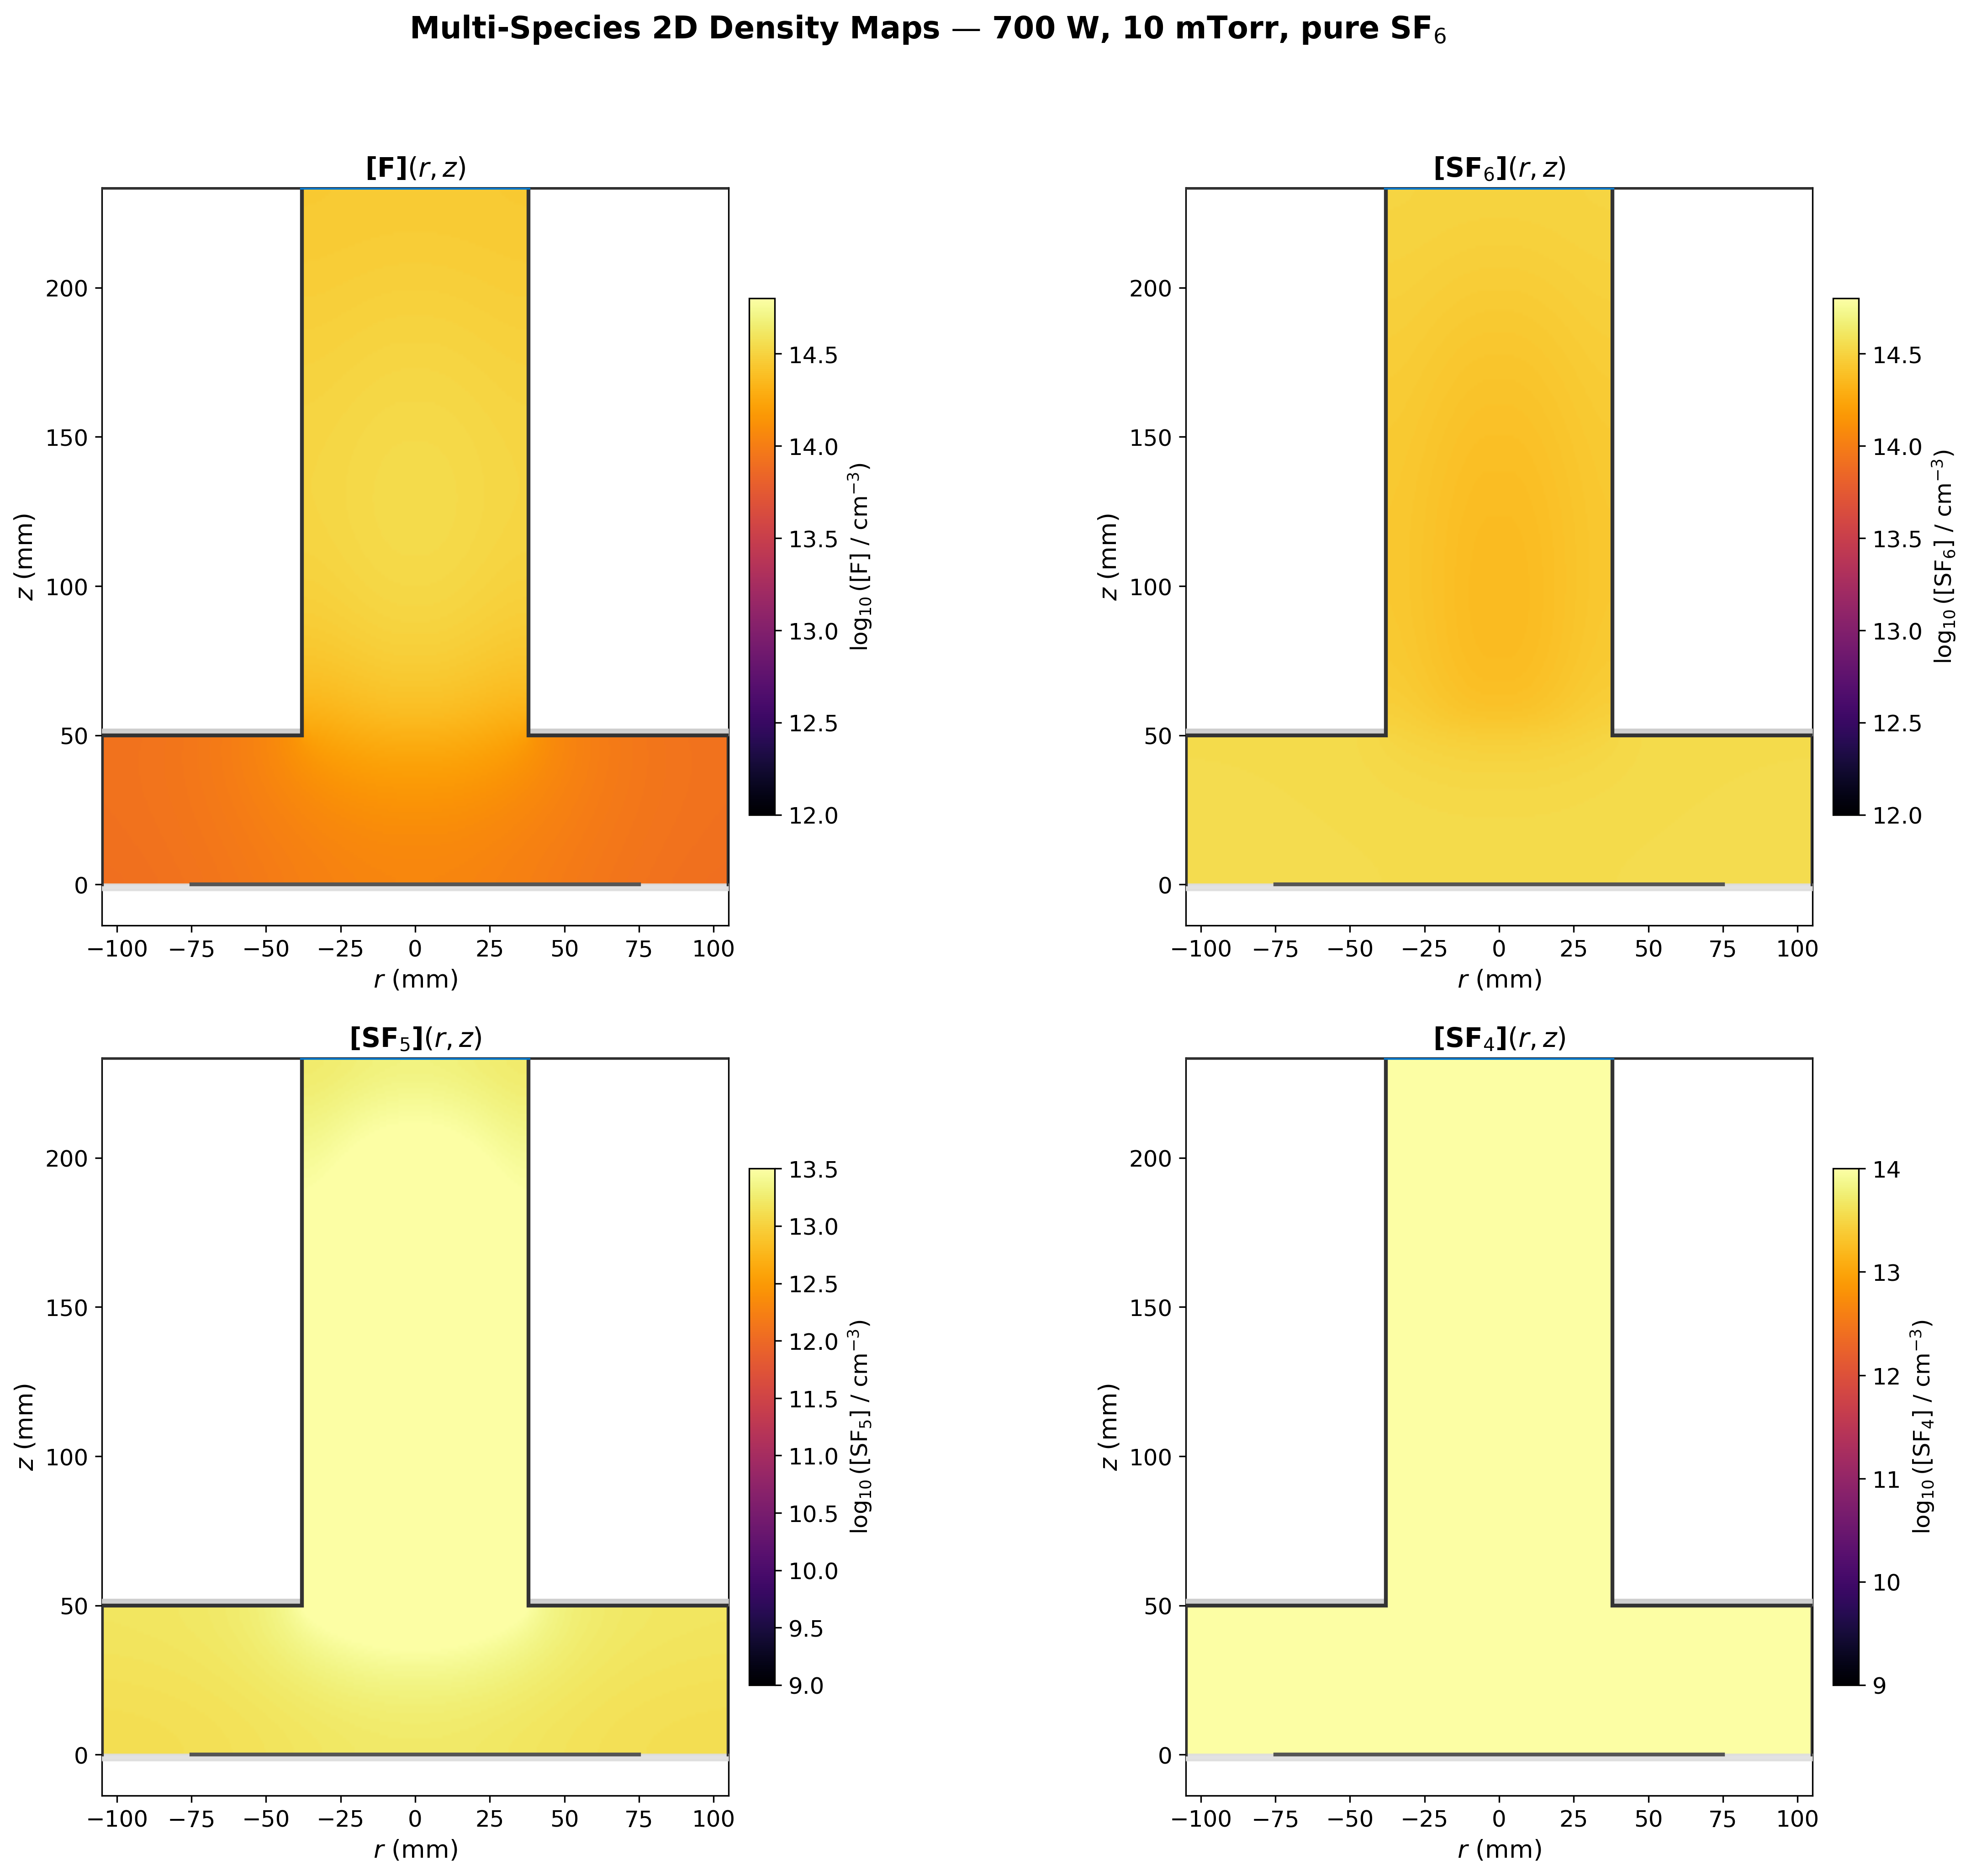
\includegraphics[width=\textwidth]{multispecies_contours.png}
  \caption{Two-dimensional density contours for major neutral and
           charged species at a representative operating point.
           Fluorine atoms are generated predominantly in the ICP
           source and diffuse through the aperture to the processing
           region.}
  \label{fig:contours}
\end{figure}

\begin{figure}[H]
  \centering
  \begin{subfigure}[t]{0.48\textwidth}
    \centering
    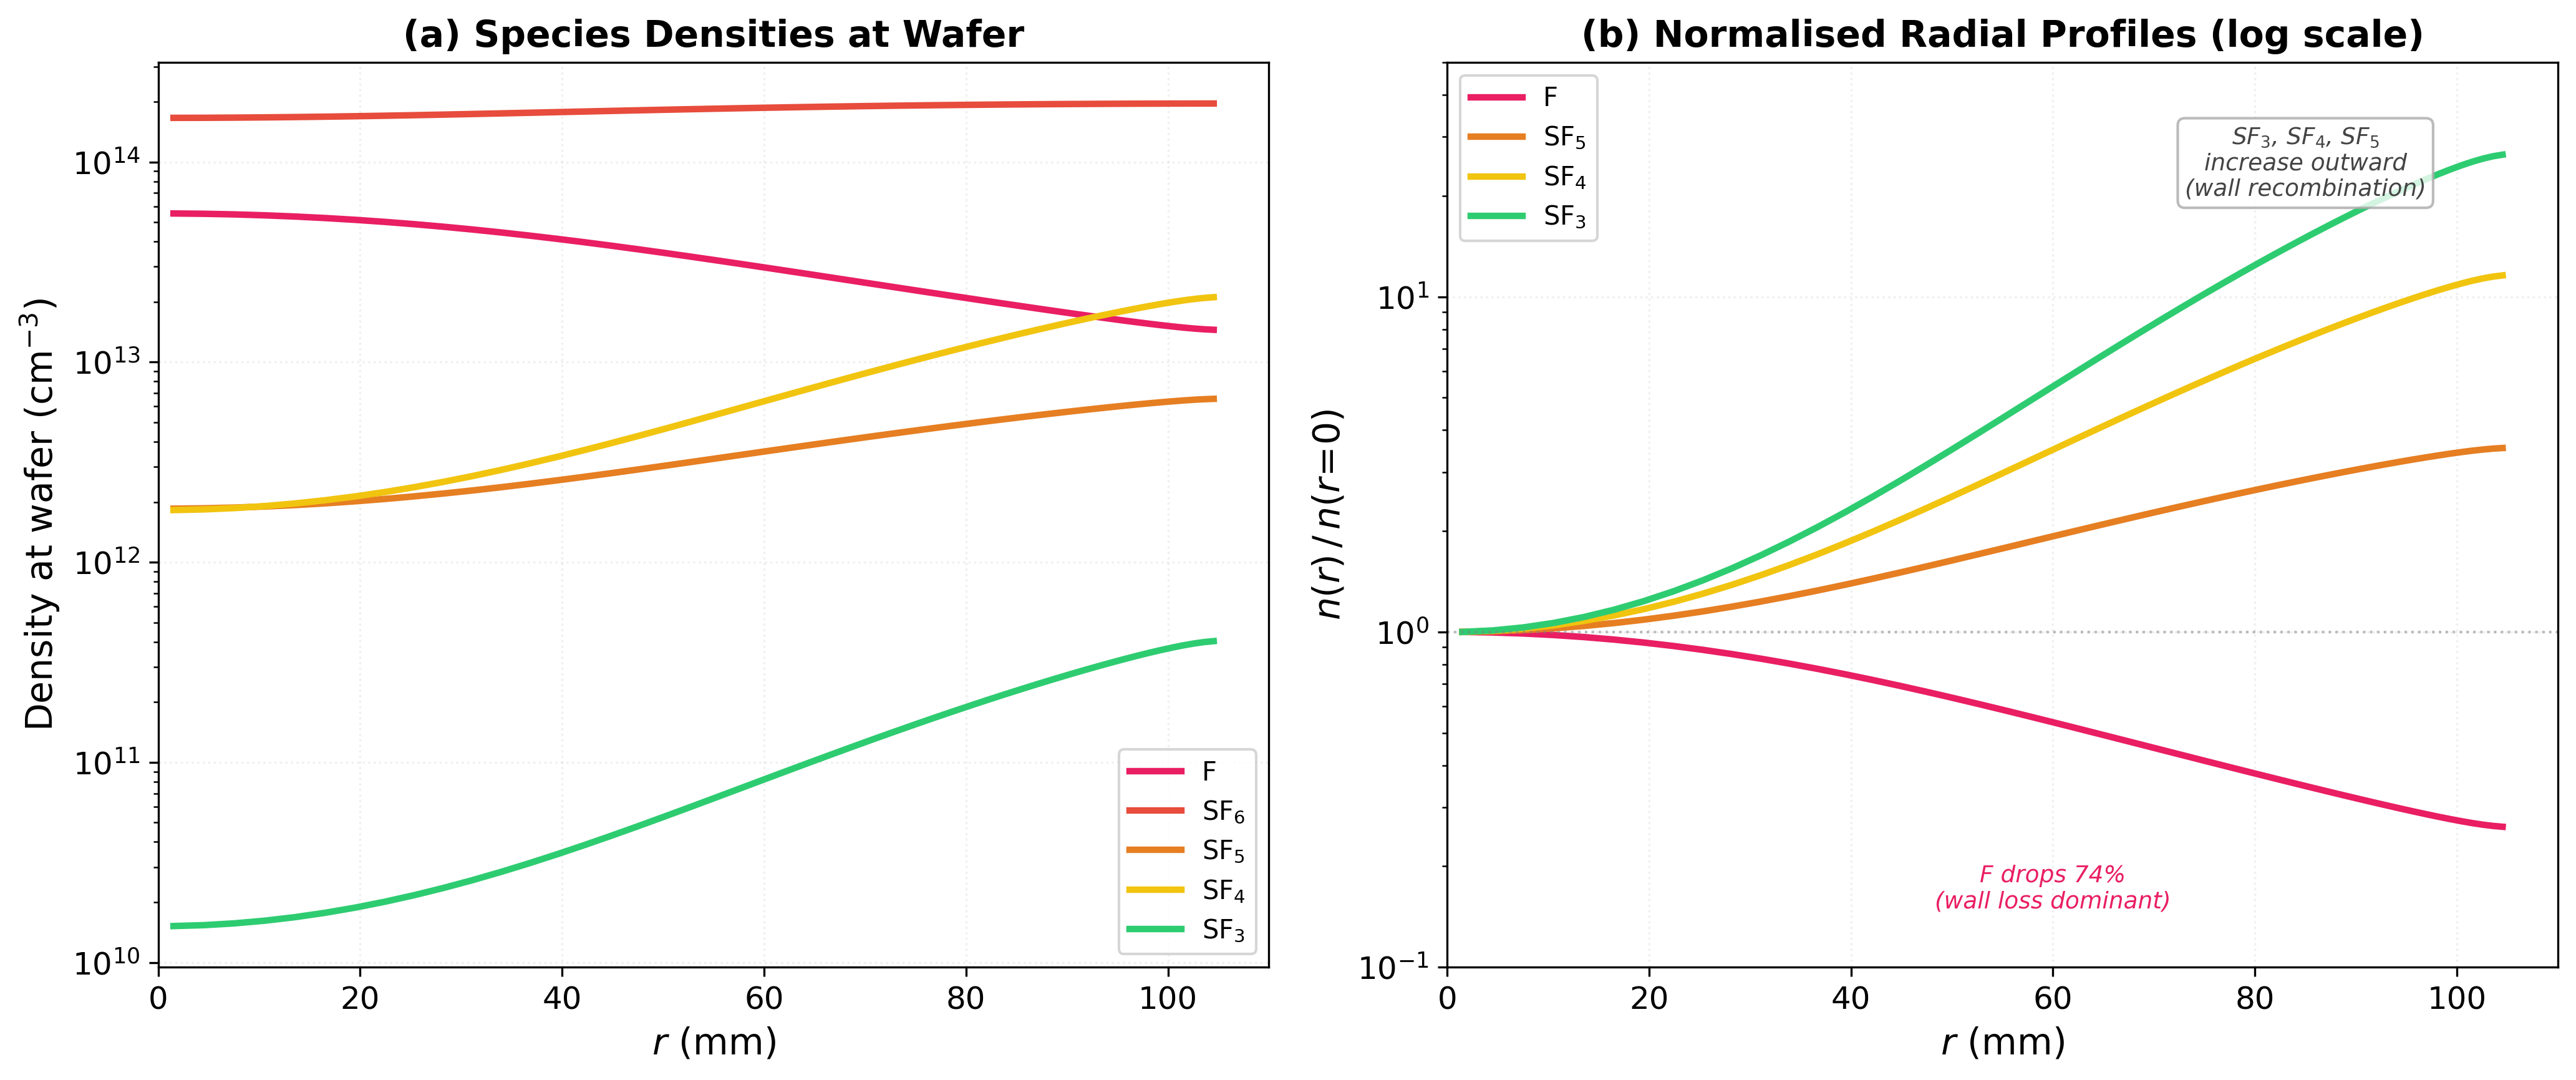
\includegraphics[width=\textwidth]{multispecies_radial.png}
    \caption{Radial profiles at the wafer surface.}
    \label{fig:radial_multi}
  \end{subfigure}
  \hfill
  \begin{subfigure}[t]{0.48\textwidth}
    \centering
    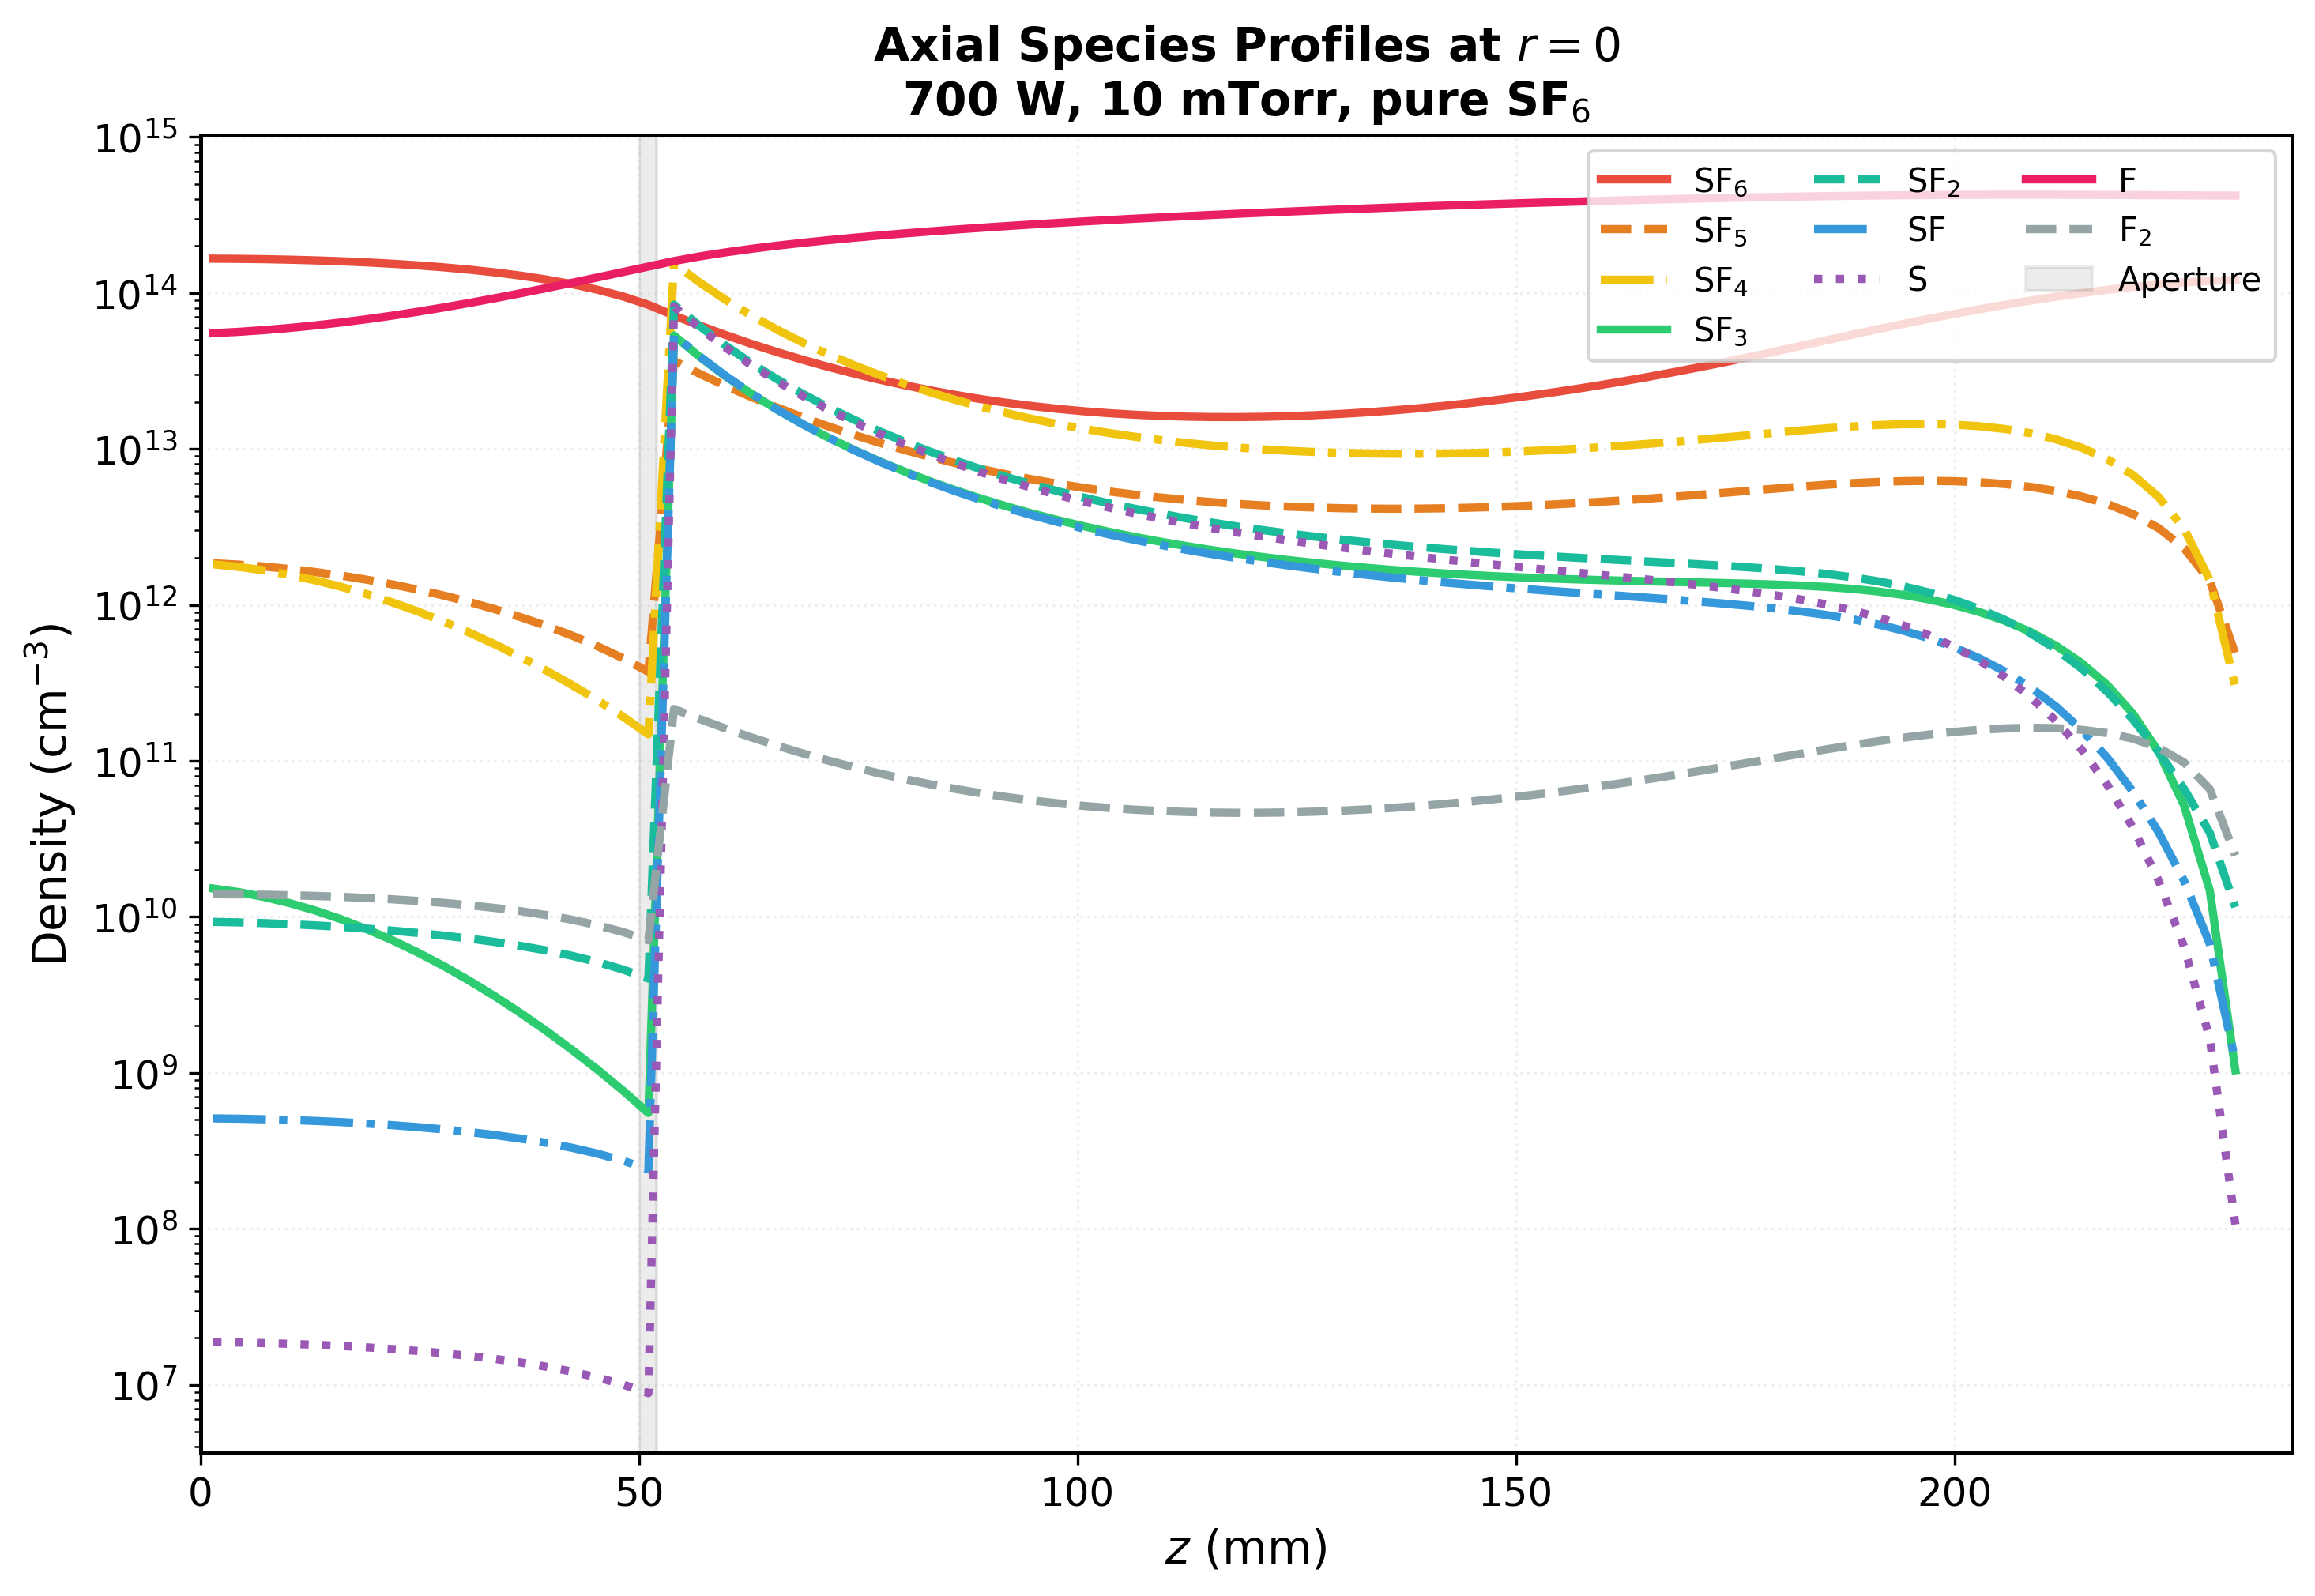
\includegraphics[width=\textwidth]{multispecies_axial.png}
    \caption{Axial profiles along the reactor centreline.}
    \label{fig:axial_multi}
  \end{subfigure}
  \caption{One-dimensional species profiles extracted from the 2D
           solution.}
  \label{fig:1d_profiles}
\end{figure}

\begin{figure}[H]
  \centering
  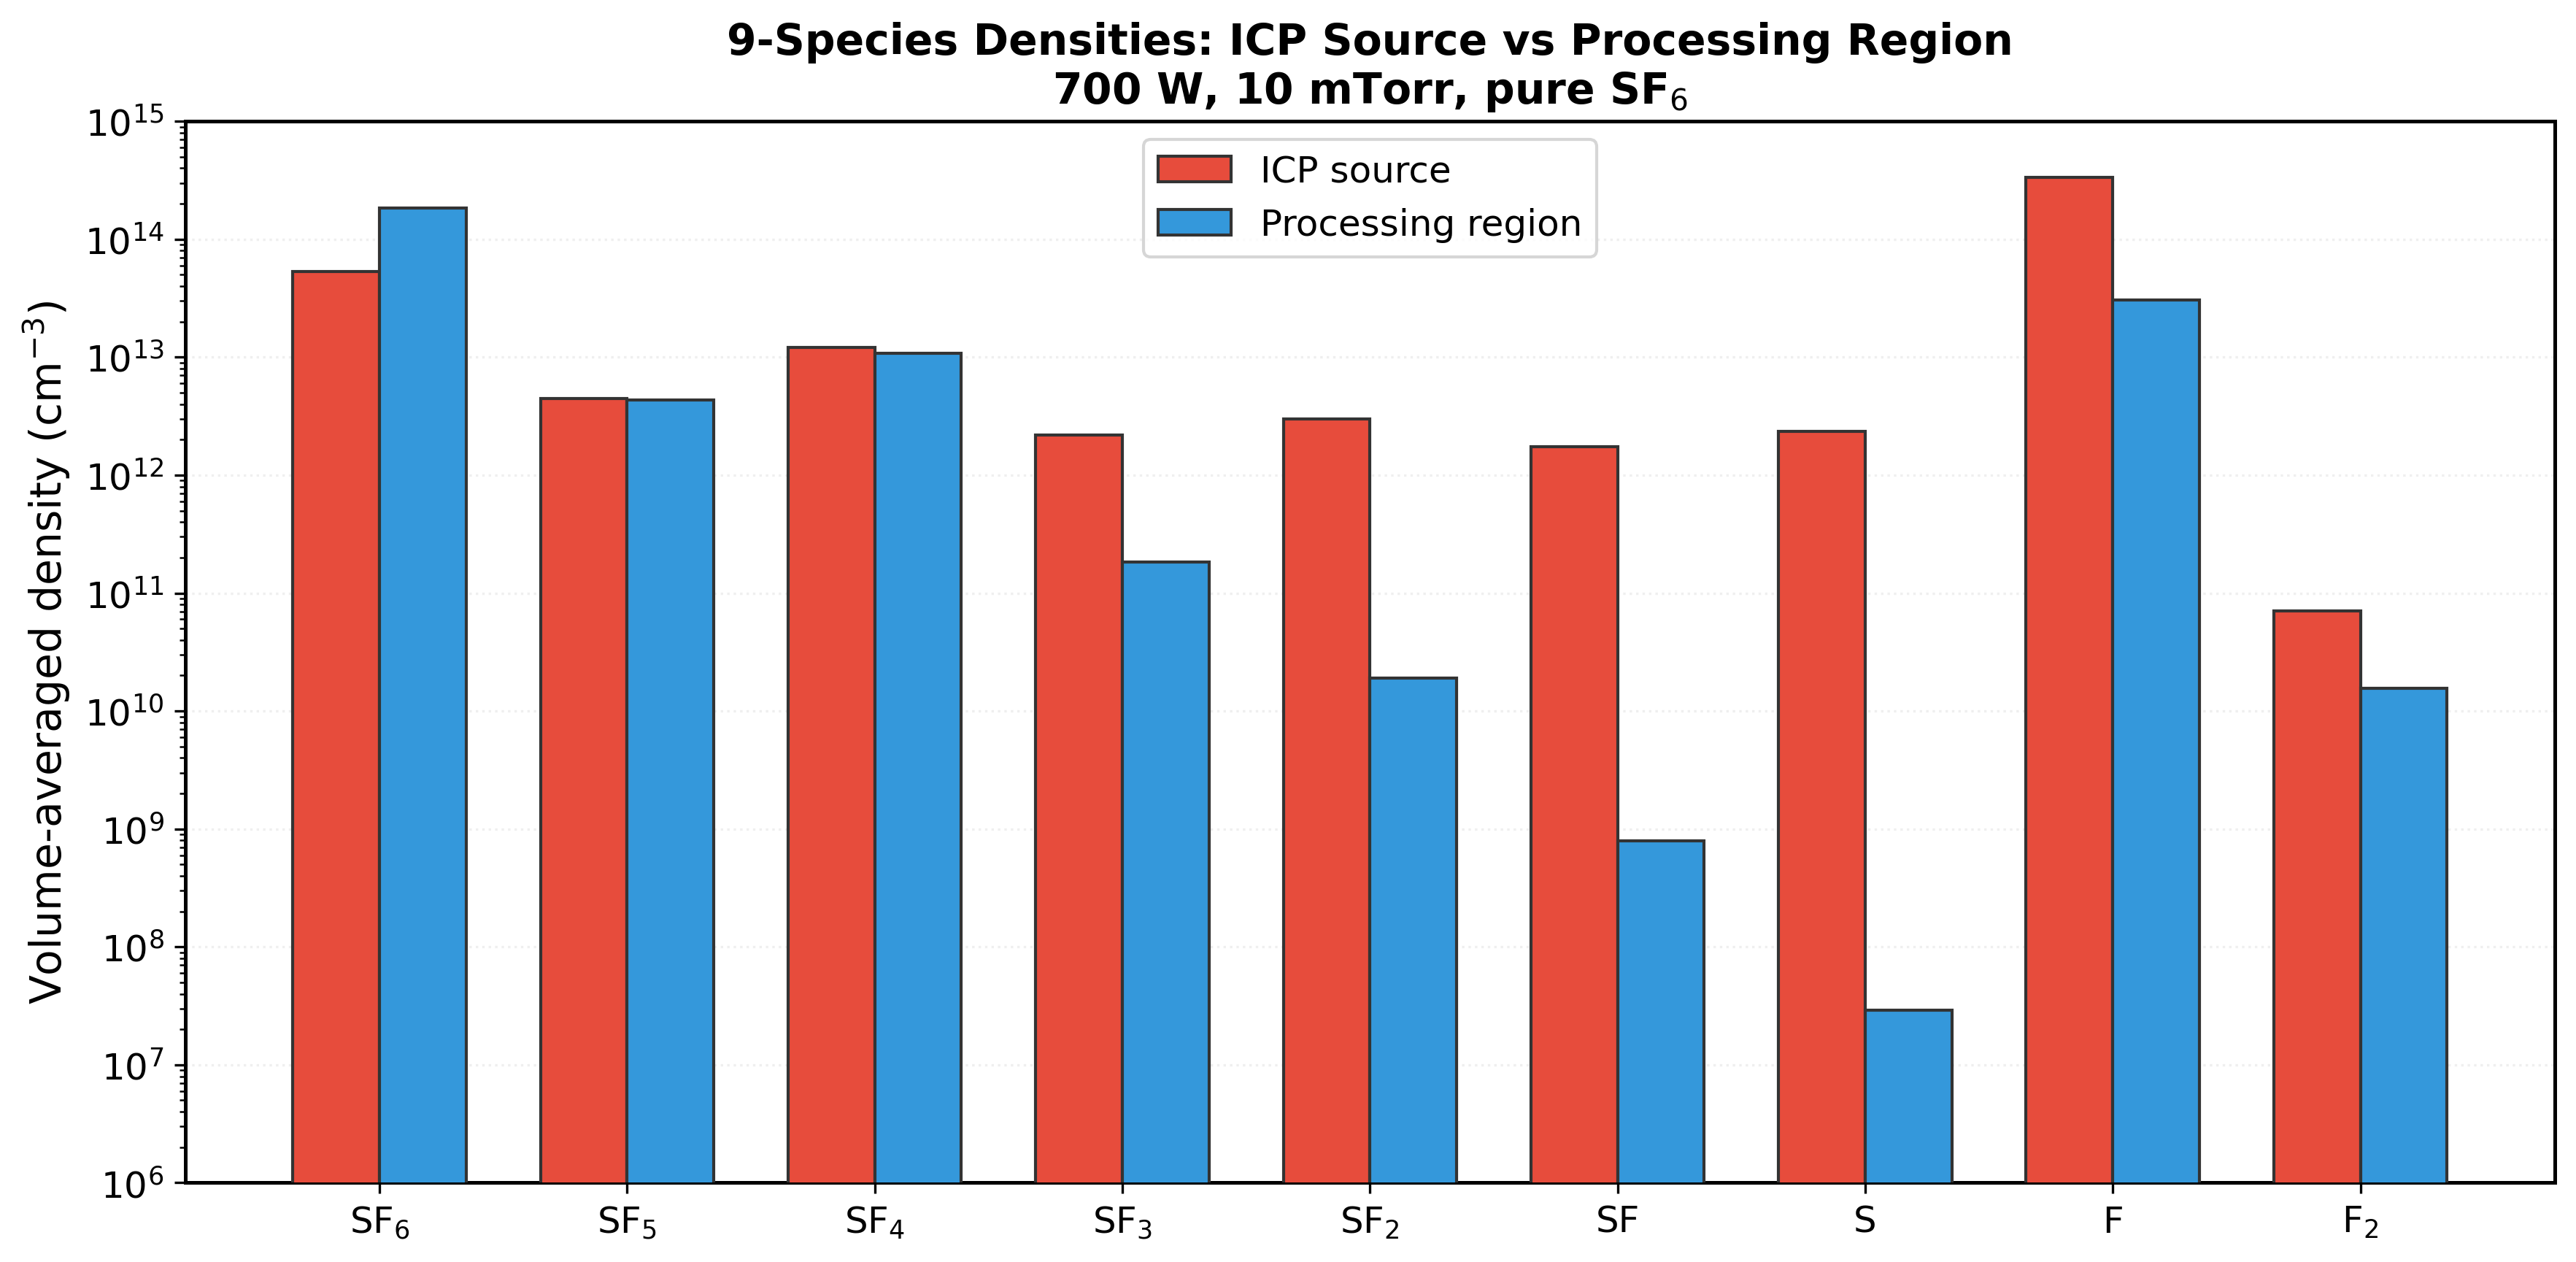
\includegraphics[width=0.65\textwidth]{multispecies_bars.png}
  \caption{Volume-averaged species densities comparing neutral and
           charged species abundances.  SF\textsubscript{6} and F
           dominate the neutral inventory; electrons and
           SF\textsubscript{5}\textsuperscript{$-$} are the
           primary charge carriers.}
  \label{fig:bars}
\end{figure}

% ==================================================================
\section{PINN Attempt: A Negative Result}
\label{sec:pinn}

The first direction pursued after validating the solver was to
accelerate it using physics-informed neural networks
(PINNs)~\citep{raissi2019}, which embed the governing PDEs directly
into the training loss.  The idea was attractive: if the network
could learn to satisfy the continuity, drift--diffusion, and energy
equations without labelled data, it would be both fast and
physically consistent.

\subsection{Data-Only Baseline}

As a sanity check, training with data loss alone converges reliably,
achieving a $23{,}000\times$ loss reduction over the training run.
This confirmed that the network architecture and optimiser were
sound, and that any subsequent failure was attributable to the PDE
loss terms.

\subsection{PDE-Constrained Training}

Adding the PDE residual to the loss function causes \textbf{training
to diverge}.  Root-cause analysis identified five interacting failure
modes:

\begin{enumerate}
  \item \textbf{Stiff chemistry:} rate coefficients span 15+ orders
        of magnitude ($\sim 10^{-22}$ to $10^{-7}$~cm$^3$/s),
        creating extreme loss-landscape curvature that defeats
        gradient-based optimisation.
  \item \textbf{Second-derivative instability:} the diffusion operator
        requires second spatial derivatives of the network output,
        amplifying noise in the automatic-differentiation graph and
        producing oscillatory gradients.
  \item \textbf{Axis singularity:} the $1/r$ term in the cylindrical
        divergence diverges at $r = 0$, creating infinite PDE
        residuals on the symmetry axis.
  \item \textbf{Coupled energy equation:} the electron temperature
        couples nonlinearly to all rate coefficients through
        Arrhenius exponentials, creating feedback loops in the PDE
        residual that amplify small $T_e$ errors.
  \item \textbf{Multi-scale loss:} the PDE residuals for different
        species differ by orders of magnitude (e.g., electron
        continuity vs.\ neutral diffusion), making balanced
        gradient descent infeasible with standard weighting.
\end{enumerate}

These findings constitute a \textbf{clear negative result}: PINNs in
their standard form are not suitable for multi-species,
stiff-chemistry plasma models in cylindrical geometry.  This failure
motivated the pivot to purely supervised surrogate training, which is
the subject of the following sections.

% ==================================================================
\section{Surrogate Development: v1 through v4}
\label{sec:surrogate}

Having established that PINNs diverge, we turned to a data-driven
supervised surrogate.  The development progressed through four
generations, each addressing a specific deficiency identified in the
previous version.

\subsection{Problem Formulation}

The surrogate is a feedforward neural network
$f_\theta : \mathbb{R}^5 \to \mathbb{R}^2$ mapping
\begin{equation}
  (r,\, z,\, P_{\text{rf}},\, p,\, x_{\text{Ar}})
  \;\longmapsto\;
  \bigl(\log_{10} n_{\text{F}},\;
         \log_{10} n_{\text{SF}_6}\bigr).
  \label{eq:surrogate_map}
\end{equation}
Working in log-density space compresses the dynamic range and
naturally enforces positivity.

\subsection{Input Features: Fourier Encoding}

The five raw inputs are augmented with random Fourier features:
\begin{equation}
  \phi(\mathbf{x}) =
  \bigl[\cos(2\pi \mathbf{B}\mathbf{x}),\;
         \sin(2\pi \mathbf{B}\mathbf{x})\bigr],
  \label{eq:fourier}
\end{equation}
where $\mathbf{B} \in \mathbb{R}^{64 \times 5}$ is sampled from
$\mathcal{N}(0, \sigma^2)$ with $\sigma = 3.0$ and held fixed during
training.  This produces a 128-dimensional feature vector that
allows the MLP to represent high-frequency spatial structure
without requiring excessive depth.

\subsection{Surrogate Progression}

Table~\ref{tab:progression} summarises the four generations.

\begin{table}[H]
  \centering
  \caption{Surrogate development progression.  Each version
           addresses a specific deficiency of its predecessor.}
  \label{tab:progression}
  \begin{tabular}{lcl}
    \toprule
    Version & nF RMSE & Key improvement \\
    \midrule
    v1 & 0.133 & Initial MLP + Fourier features \\
    v2 & 0.111 & Data enrichment (more operating points) \\
    v3 & 0.023 & Physics regularisation (smoothness, bounds) \\
    v4 & 0.003 & Output-bias initialisation + ensemble UQ \\
    \bottomrule
  \end{tabular}
\end{table}

The jump from v2 to v3 (0.111 $\to$ 0.023, a $4.8\times$ reduction)
came from adding physics-based regularisation terms.  The further jump
from v3 to v4 (0.023 $\to$ 0.003, a $7.7\times$ reduction) came
primarily from output-bias initialisation, as confirmed by the
ablation study in Section~\ref{sec:ablation}.  Together these
represent a $44\times$ improvement from v1 to v4.

The v4 surrogate achieves a $531\times$ speedup over the legacy
solver (\SI{14.6}{\milli\second} vs.\ \SI{7.76}{\second}).

\subsection{Physics-Based Regularisation}

Three regularisation terms are added to the MSE data loss:

\paragraph{Smoothness penalty.}
Penalises large spatial gradients to suppress unphysical oscillations:
\begin{equation}
  \mathcal{L}_{\text{smooth}}
  = \lambda_{\text{smooth}}
    \left\langle
      \left|\frac{\partial \hat{y}}{\partial r}\right|^2
      + \left|\frac{\partial \hat{y}}{\partial z}\right|^2
    \right\rangle,
  \quad \lambda_{\text{smooth}} = 5 \times 10^{-4}.
  \label{eq:smooth}
\end{equation}

\paragraph{Bounded-density penalty.}
Penalises predictions outside the physically plausible range:
\begin{equation}
  \mathcal{L}_{\text{bound}}
  = \lambda_{\text{bound}}
    \left\langle
      \max(0,\, \hat{y} - y_{\max})^2
      + \max(0,\, y_{\min} - \hat{y})^2
    \right\rangle,
  \quad \lambda_{\text{bound}} = 1 \times 10^{-3}.
  \label{eq:bound}
\end{equation}

\paragraph{Wafer-smoothness penalty.}
An additional smoothness penalty specific to the wafer plane:
\begin{equation}
  \mathcal{L}_{\text{wafer}}
  = \lambda_{\text{wafer}}
    \left\langle
      \left|\frac{\partial \hat{y}}{\partial r}\right|^2
      \bigg|_{z = z_{\text{wafer}}}
    \right\rangle,
  \quad \lambda_{\text{wafer}} = 2 \times 10^{-4}.
  \label{eq:wafer_smooth}
\end{equation}

\subsection{Output Bias Initialisation}

The final bias of each head is initialised to the log-mean of the
corresponding species density across the training set:
\begin{equation}
  b_{\text{F}}^{(0)} = 19.8, \qquad
  b_{\text{SF}_6}^{(0)} = 20.0.
  \label{eq:bias_init}
\end{equation}
This ensures that the network output starts near the correct order of
magnitude ($\sim 10^{19}$--$10^{20}\;\si{\per\cubic\metre}$),
dramatically accelerating convergence.  As shown in
Section~\ref{sec:ablation}, this single design choice accounts for
83\% of the total RMSE improvement.

% ==================================================================
\section{LXCat Cross-Section Integration}
\label{sec:lxcat}

\subsection{Motivation and Implementation}

The legacy solver uses tabulated electron-impact cross sections.
To improve traceability, we integrated the Biagi-v10.6
dataset~\citep{biagi} from the LXCat platform~\citep{lxcat}.  The
Biagi cross sections were parsed from the LXCat database format, and
Maxwellian-averaged rate coefficients were computed as functions of
electron temperature.  The solver was modified to support a
\texttt{rate\_mode='lxcat'} flag that selects between the legacy
tabulated rates and the new LXCat-derived rates.

\begin{figure}[H]
  \centering
  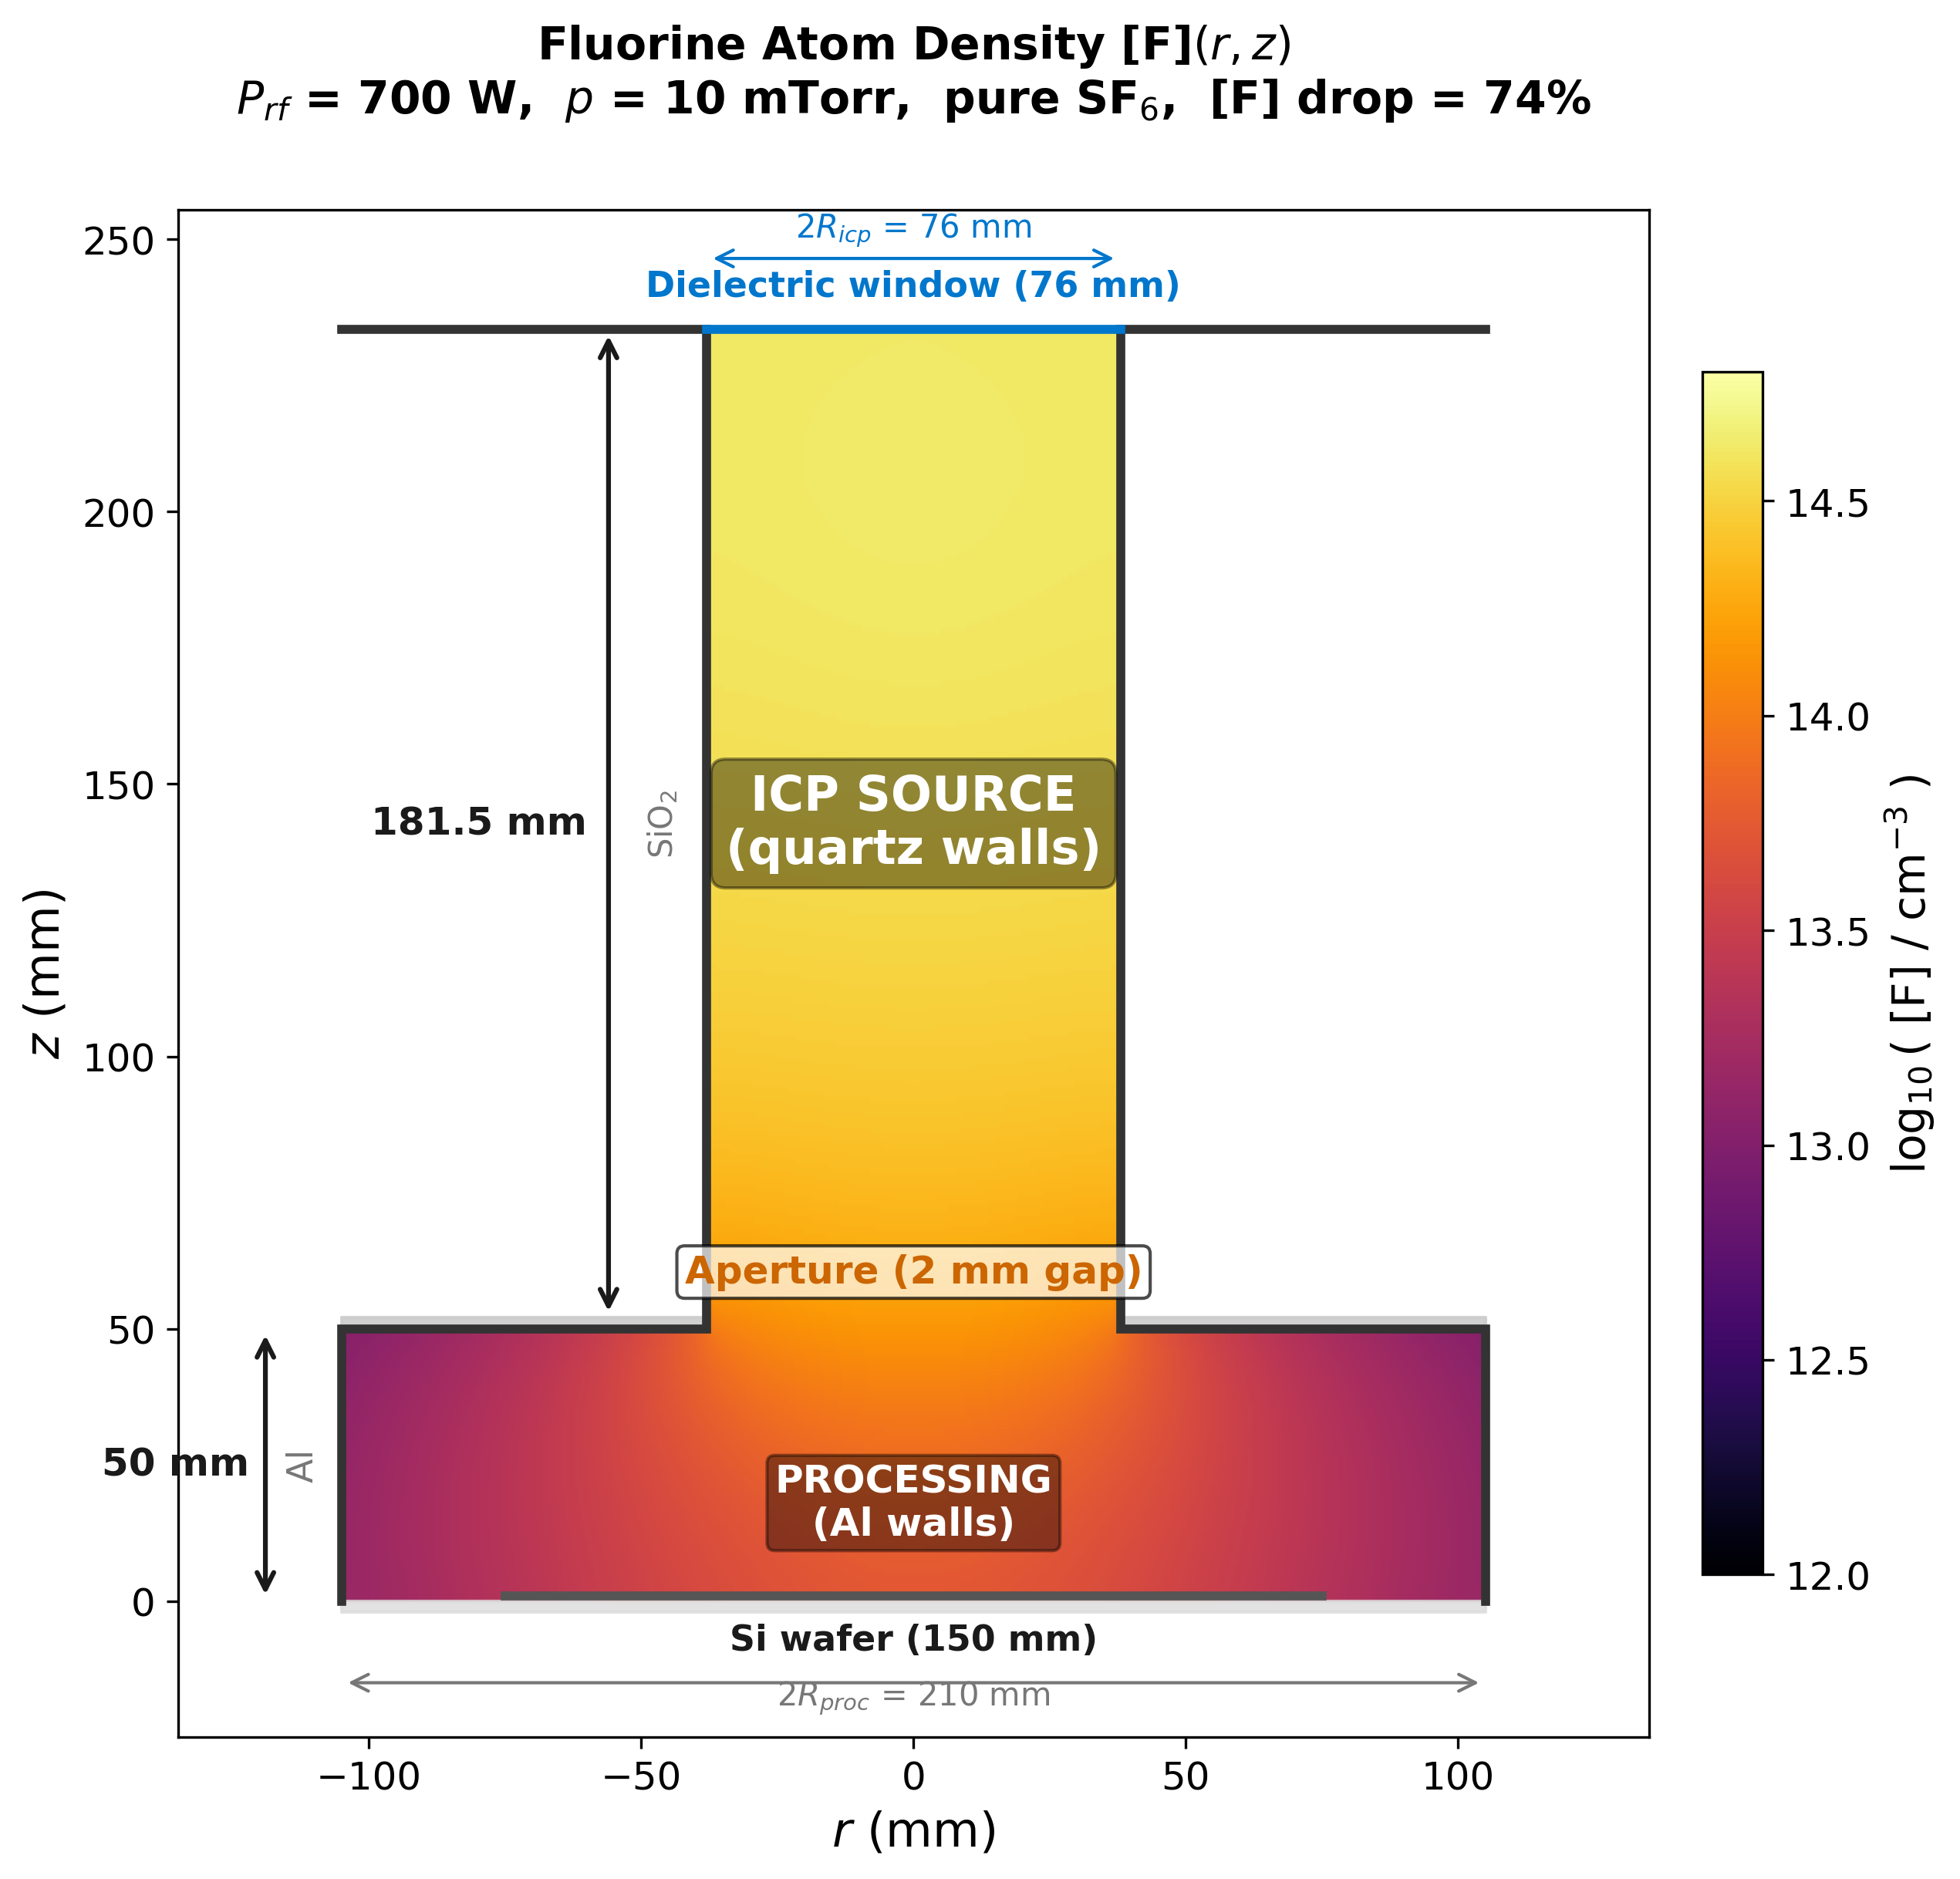
\includegraphics[width=0.65\textwidth]{cross_sections.png}
  \caption{Electron-impact cross sections for key SF\textsubscript{6}
           processes from the Biagi-v10.6 dataset.  The dominant channels
           are dissociative attachment and vibrational excitation at
           low electron energies, and ionisation at higher energies.}
  \label{fig:cross_sections}
\end{figure}

\subsection{Rate Coefficient Comparison}

Figure~\ref{fig:rate_comparison} compares selected rate coefficients
between the legacy and LXCat sets.  The differences are most
pronounced for dissociative attachment at low $E/N$, which is the
dominant source of F atoms.

\begin{figure}[H]
  \centering
  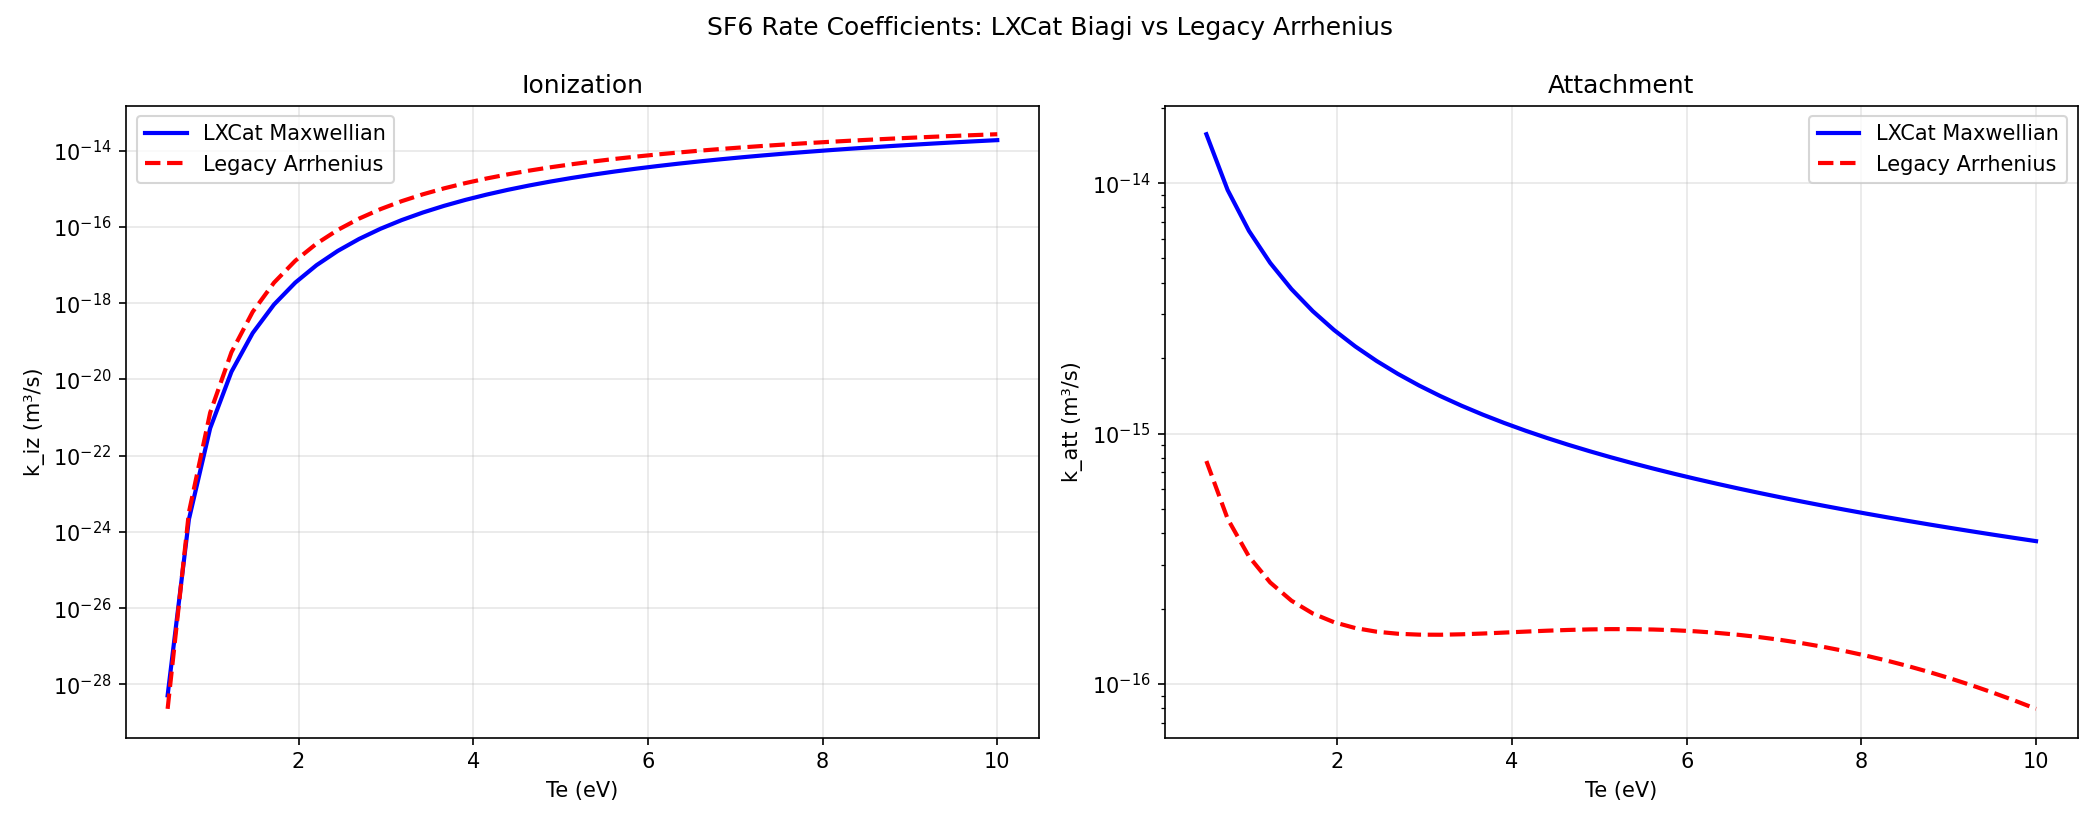
\includegraphics[width=0.65\textwidth]{lxcat_rate_comparison.png}
  \caption{Comparison of selected electron-impact rate coefficients
           computed from legacy tabulated cross sections versus the
           LXCat/Biagi-v10.6 set.  Differences are most pronounced for
           dissociative attachment at low $E/N$.}
  \label{fig:rate_comparison}
\end{figure}

\subsection{Physics Impact}

The LXCat solver produces dramatically different plasma parameters at
the same operating conditions:
\begin{itemize}
  \item \textbf{Electron temperature:} $T_e$ increases by \textbf{56\%}.
        The Biagi cross sections have lower inelastic loss rates at the
        relevant energies, requiring a higher $T_e$ to sustain the
        discharge.
  \item \textbf{Electron density:} $n_e$ decreases by \textbf{69\%},
        consistent with the higher $T_e$ (fewer electrons needed at
        higher mean energy to maintain ionisation balance).
  \item \textbf{F density:} unchanged within numerical accuracy.
        The dissociation rate adjusts to compensate for the $T_e$ and
        $n_e$ shifts.
\end{itemize}
The invariance of F density despite large shifts in $T_e$ and $n_e$
is a surprising and physically meaningful result: it suggests that
the F density is controlled primarily by transport (diffusion through
the aperture and wall recombination) rather than by the details of
electron-impact kinetics.

Figure~\ref{fig:lxcat_wafer} shows the radial F density profile at
the wafer from the LXCat solver.

\begin{figure}[H]
  \centering
  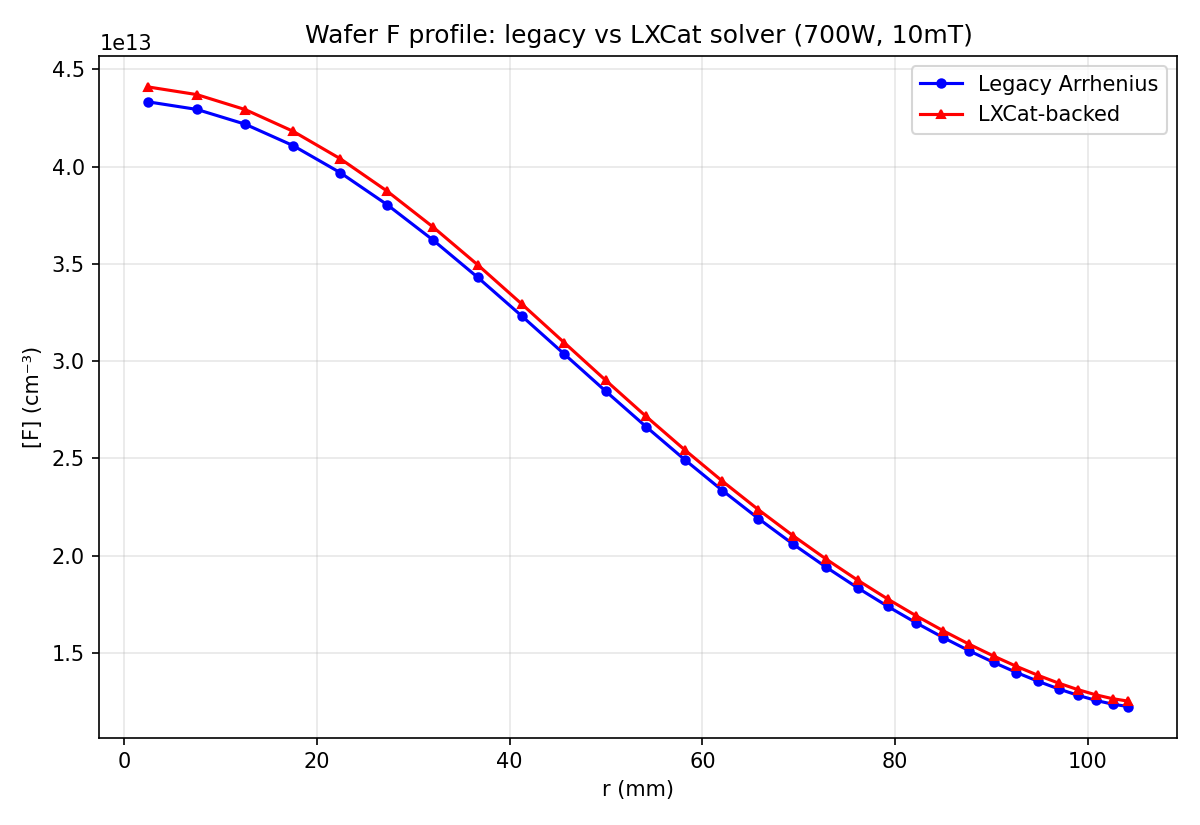
\includegraphics[width=0.6\textwidth]{lxcat_solver_wafer_profile.png}
  \caption{Radial F density profile at the wafer predicted by the
           LXCat solver.  The profile shape is similar to the legacy
           solver; absolute densities are nearly identical despite
           the large $T_e$ and $n_e$ shifts.}
  \label{fig:lxcat_wafer}
\end{figure}

\subsection{Dataset Diagnosis: Recipe, Not Physics}
\label{sec:dataset_diagnosis}

When the v4 training recipe was applied to LXCat data, the initial
RMSE was $3.85\times$ worse than on legacy data.  A natural hypothesis
was that the LXCat data are intrinsically harder to learn.  We tested
this by comparing the statistical properties of the two datasets:
\begin{itemize}
  \item Log-density standard deviation ratio: $0.99\times$.
  \item Gradient P90 ratio: $0.99\times$.
  \item Correlation shift: $< 0.003$.
\end{itemize}
The two datasets are \textbf{statistically identical} in difficulty.
The $3.85\times$ RMSE gap was entirely attributable to the training
recipe (architecture, initialisation, regularisation), not to any
difference in the underlying data distributions.  This finding
motivated the architecture sweep described in the next section.

% ==================================================================
\section{Architecture Sweep}
\label{sec:arch_sweep}

Having established that the performance gap was a recipe problem, we
conducted a controlled architecture sweep to find the best topology
for the LXCat dataset.

\subsection{Experimental Design}

Seven architectures (E0--E6) were evaluated, each trained with three
random seeds on the LXCat dataset under identical training budgets.
Table~\ref{tab:arch_sweep} reports the mean and standard deviation
of the normalised F-density RMSE.

\begin{table}[H]
  \centering
  \caption{Architecture sweep results (LXCat dataset, 3 seeds each).
           RMSE values are normalised.}
  \label{tab:arch_sweep}
  \begin{tabular}{llcc}
    \toprule
    ID & Architecture & nF RMSE & $\pm\,1\sigma$ \\
    \midrule
    E0 & Baseline (no reg, 1500 ep)
       & 0.01901 & 0.00393 \\
    E1 & V4 recipe (reg + bias + 2000 ep)
       & 0.00377 & 0.00056 \\
    E2 & Wider/deeper ($6\times256$ + reg)
       & 0.00390 & 0.00099 \\
    E3 & \textbf{Separate heads} (trunk + heads + reg)
       & \textbf{0.00210} & \textbf{0.00015} \\
    E4 & Residual (res blocks + reg)
       & 0.00244 & 0.00066 \\
    E5 & Enhanced features (10 inputs + reg)
       & 0.00957 & 0.00180 \\
    E6 & Huber loss (Huber + reg)
       & 0.00394 & 0.00083 \\
    \bottomrule
  \end{tabular}
\end{table}

\subsection{Analysis}

\textbf{E3\_separate\_heads} achieves the lowest mean RMSE (0.00210)
with the smallest seed-to-seed variance ($\sigma = 0.00015$),
indicating both accuracy and training stability.  Key observations:
\begin{itemize}
  \item E4 (residual) is a close second but with $4.4\times$ larger
        variance, making it less reliable.
  \item Simply making the network wider and deeper (E2) provides no
        benefit over the v4 recipe (E1), confirming that capacity is
        not the bottleneck.
  \item Expanding the feature set (E5) \emph{hurts} performance
        ($4.6\times$ worse than E3), likely due to the curse of
        dimensionality on the modest training set.
  \item Huber loss (E6) offers no advantage over MSE in this
        application.
\end{itemize}

The single-model E3 nF RMSE of 0.0021 already beats the legacy v4's
0.0029, confirming that the architecture change alone closes the gap.

\subsection{E3 Architecture}

The winning architecture (Figure~\ref{fig:flowchart}) consists of:
\begin{enumerate}
  \item A \textbf{shared trunk}: 3 hidden layers of width 128 with
        ReLU activations and a skip connection from the Fourier
        features to the trunk output.
  \item \textbf{Two species-specific heads}: each a 2-layer MLP
        with width 64 and ReLU activations, producing a scalar
        output for $\log_{10} n_{\text{F}}$ and
        $\log_{10} n_{\text{SF}_6}$ respectively.
\end{enumerate}
The shared trunk captures common spatial patterns (geometry, power
deposition), while the separate heads specialise to species-specific
chemistry.

\begin{figure}[H]
  \centering
  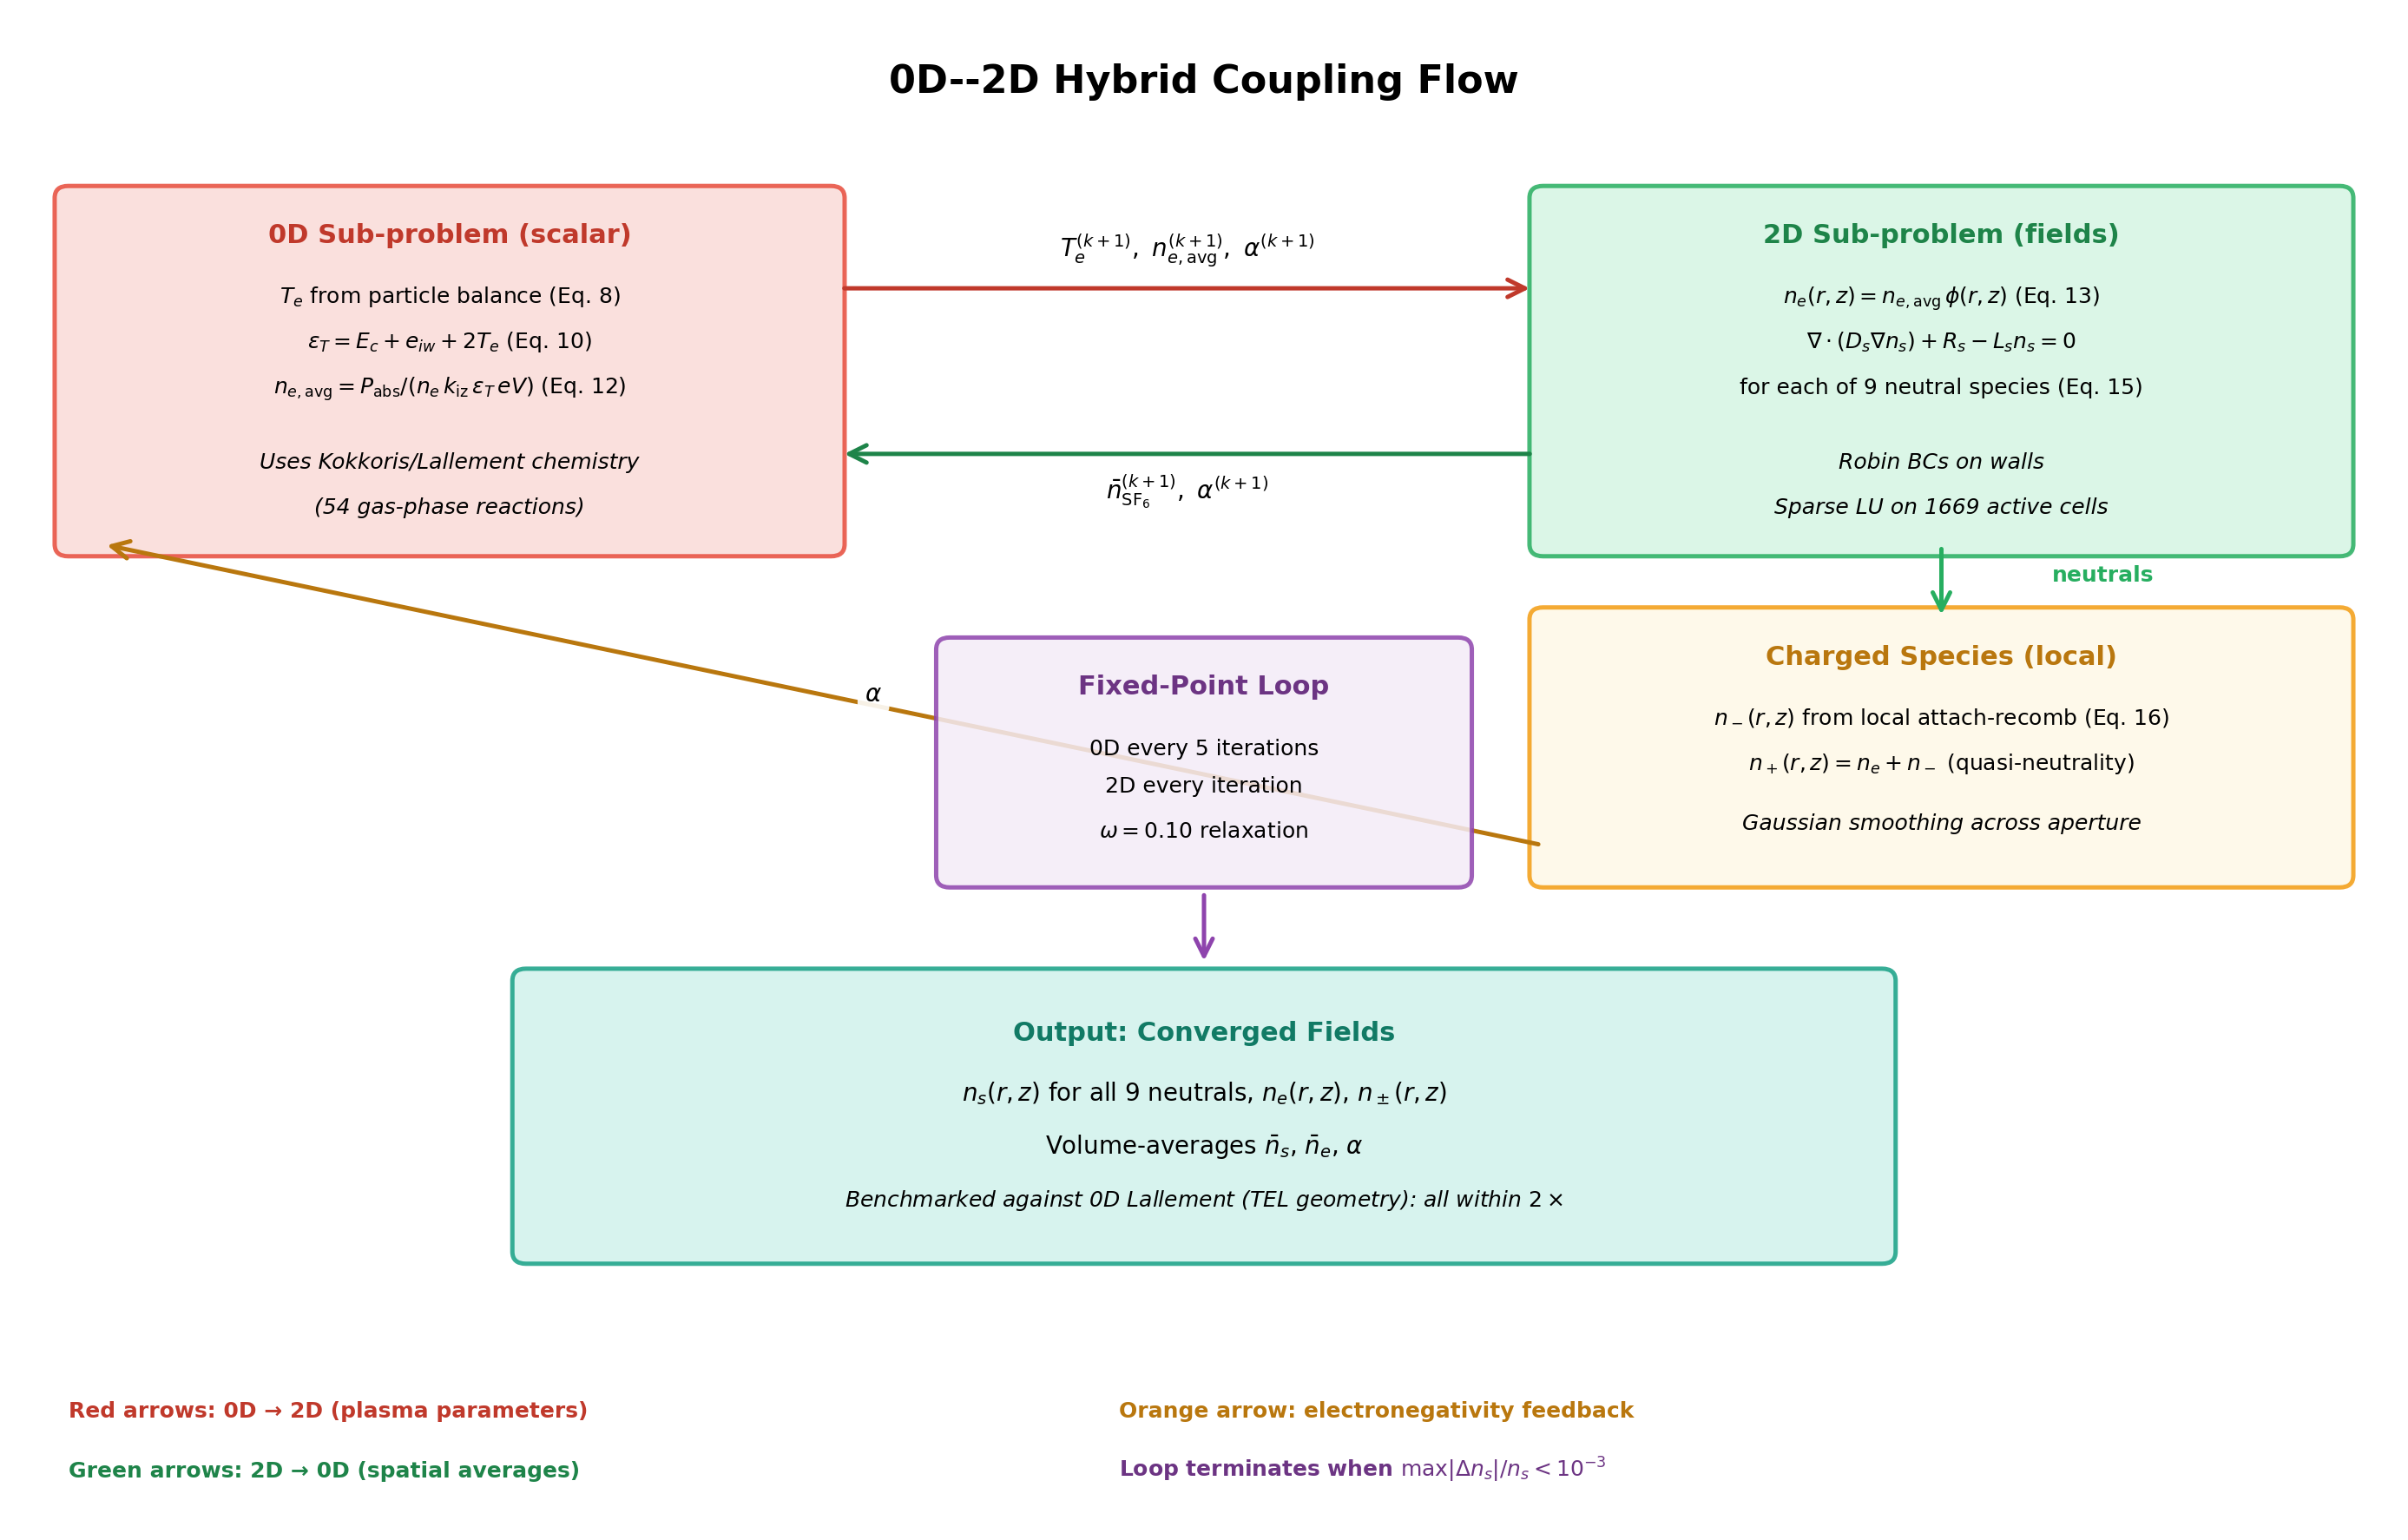
\includegraphics[width=0.55\textwidth]{coupling_flowchart.png}
  \caption{Surrogate architecture (E3\_separate\_heads).  The shared
           trunk receives Fourier-encoded inputs; a skip connection
           concatenates the raw Fourier features with the trunk output
           before feeding species-specific head networks.}
  \label{fig:flowchart}
\end{figure}

% ==================================================================
\section{Ablation Study}
\label{sec:ablation}

To disentangle the contributions of regularisation, bias
initialisation, and extended training, we ran a single-factor ablation
with five configurations (3 seeds each).  Results are in
Table~\ref{tab:ablation}.

\begin{table}[H]
  \centering
  \caption{Ablation study.  Improvement is relative to the ``none''
           baseline (nF RMSE = 0.01830).}
  \label{tab:ablation}
  \begin{tabular}{lcc}
    \toprule
    Configuration & nF RMSE & Improvement \\
    \midrule
    None (baseline)     & 0.01830 & ---   \\
    Bias only           & 0.00314 & +83\% \\
    Regularisation only & 0.01888 & $-3$\%\\
    Epochs only (2000)  & 0.01610 & +12\% \\
    All three           & 0.00385 & +79\% \\
    \bottomrule
  \end{tabular}
\end{table}

\subsection{Key Findings}

The ablation reveals a clear hierarchy:

\paragraph{Bias initialisation is the dominant factor.}
Adding output-bias initialisation alone reduces the RMSE from 0.01830
to 0.00314---an 83\% improvement.  Without this, the network spends
its first hundreds of epochs merely shifting the output mean from
near-zero to the correct order of magnitude
($\sim 10^{19}$--$10^{20}$~m$^{-3}$), during which time the spatial
structure signal is overwhelmed by the magnitude error.

\paragraph{Regularisation alone is useless.}
Adding smoothness, bounds, and wafer-smoothness penalties without bias
initialisation yields nF RMSE = 0.01888---marginally \emph{worse}
than the baseline ($-3\%$).  The regularisation constrains the spatial
structure before the network has found the correct magnitude, actually
impeding convergence.

\paragraph{Extended training provides a modest gain.}
Increasing from 1500 to 2000 epochs yields a 12\% improvement (0.01610
vs.\ 0.01830), confirming that the baseline was slightly undertrained
but that the fundamental bottleneck was initialisation, not epochs.

\paragraph{The ``all three'' configuration is slightly worse than
bias-only.}  nF RMSE = 0.00385 vs.\ 0.00314 for bias-only, because
the regularisation terms slightly increase the data-fit loss.  This
is an acceptable trade-off: the regularised model produces smoother,
more physically plausible spatial profiles despite the marginal RMSE
increase.

% ==================================================================
\section{Production Ensemble}
\label{sec:production}

The winning E3 architecture was retrained as a 5-model ensemble,
achieving:
\begin{align}
  \text{nF RMSE}              &= 0.00154, \label{eq:nf_rmse} \\
  \text{nSF}_6\text{ RMSE}    &= 0.00128. \label{eq:nsf6_rmse}
\end{align}
This represents a \textbf{47\% improvement} over the legacy
surrogate\_v4 (nF RMSE = 0.00292).  The ensemble was trained with the
Adam optimiser and cosine-annealing learning-rate schedule for 2000
epochs with a batch size of 4096.

\subsection{Diagnostics}

Figure~\ref{fig:diagnostics} shows diagnostic plots for both target
species, including residual distributions, spatial error maps, and
per-condition RMSE breakdowns.  The residuals are approximately
Gaussian with no systematic bias.

\begin{figure}[H]
  \centering
  \begin{subfigure}[t]{0.48\textwidth}
    \centering
    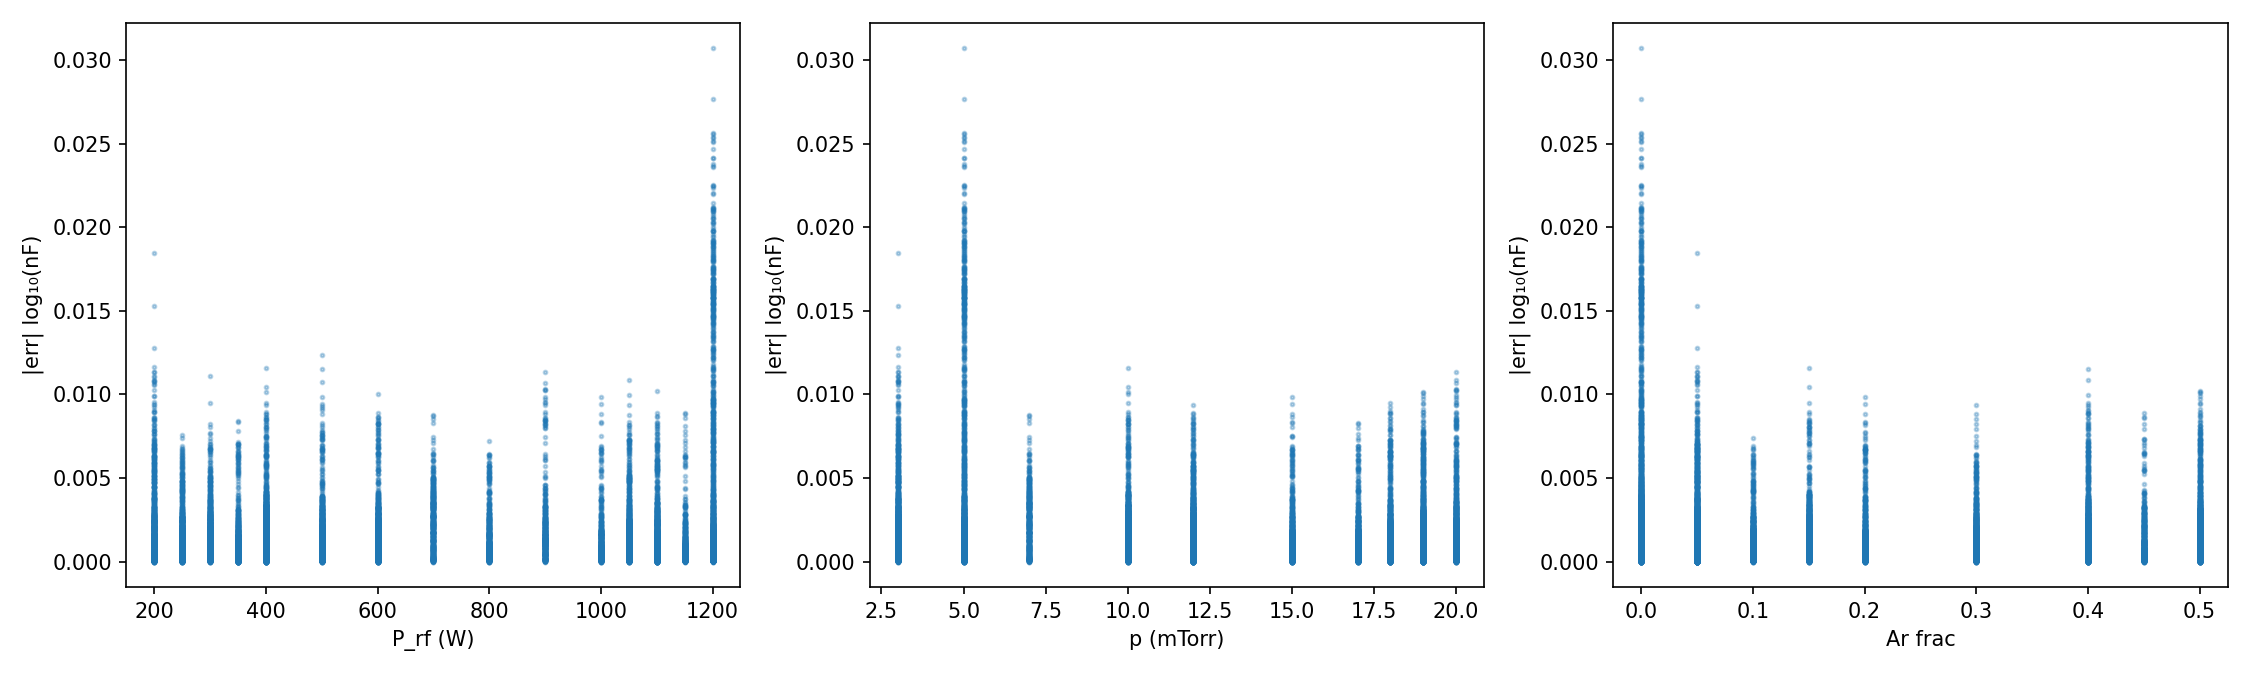
\includegraphics[width=\textwidth]{surrogate_v4_diagnostics_nF.png}
    \caption{F density diagnostics.}
    \label{fig:diag_nF}
  \end{subfigure}
  \hfill
  \begin{subfigure}[t]{0.48\textwidth}
    \centering
    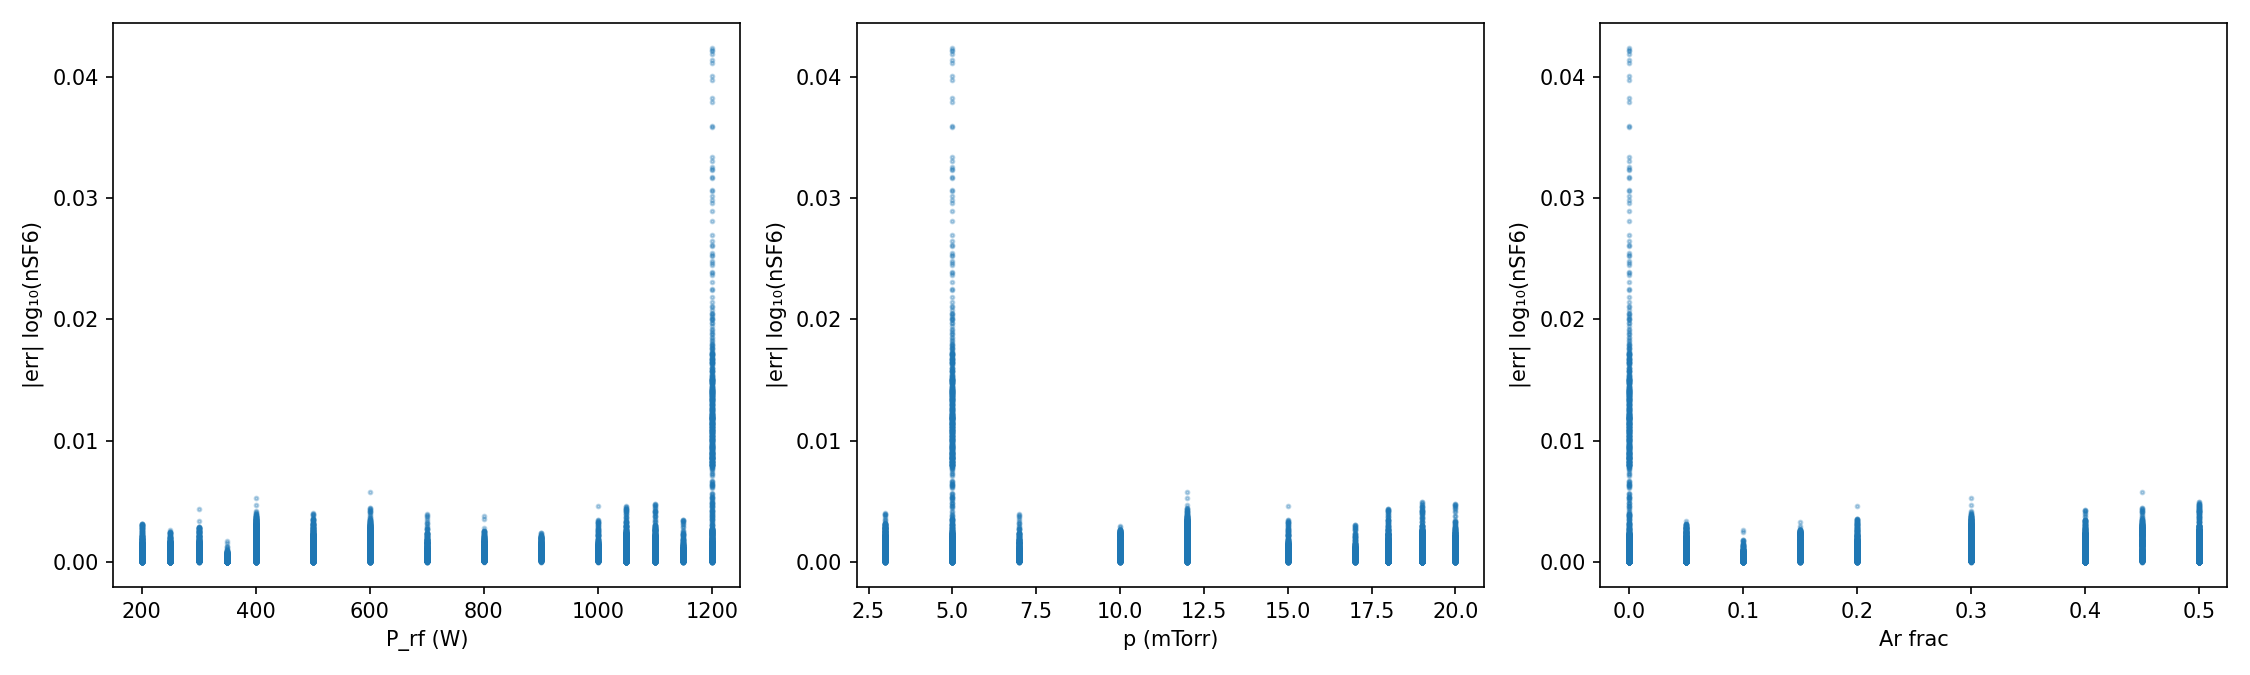
\includegraphics[width=\textwidth]{surrogate_v4_diagnostics_nSF6.png}
    \caption{SF\textsubscript{6} density diagnostics.}
    \label{fig:diag_nSF6}
  \end{subfigure}
  \caption{Surrogate diagnostic plots showing residual distributions,
           spatial error maps, and per-condition RMSE for both target
           species.}
  \label{fig:diagnostics}
\end{figure}

\subsection{Predicted vs.\ True}

Figure~\ref{fig:pred_vs_true} confirms that predictions cluster
tightly around the identity line across four orders of magnitude.

\begin{figure}[H]
  \centering
  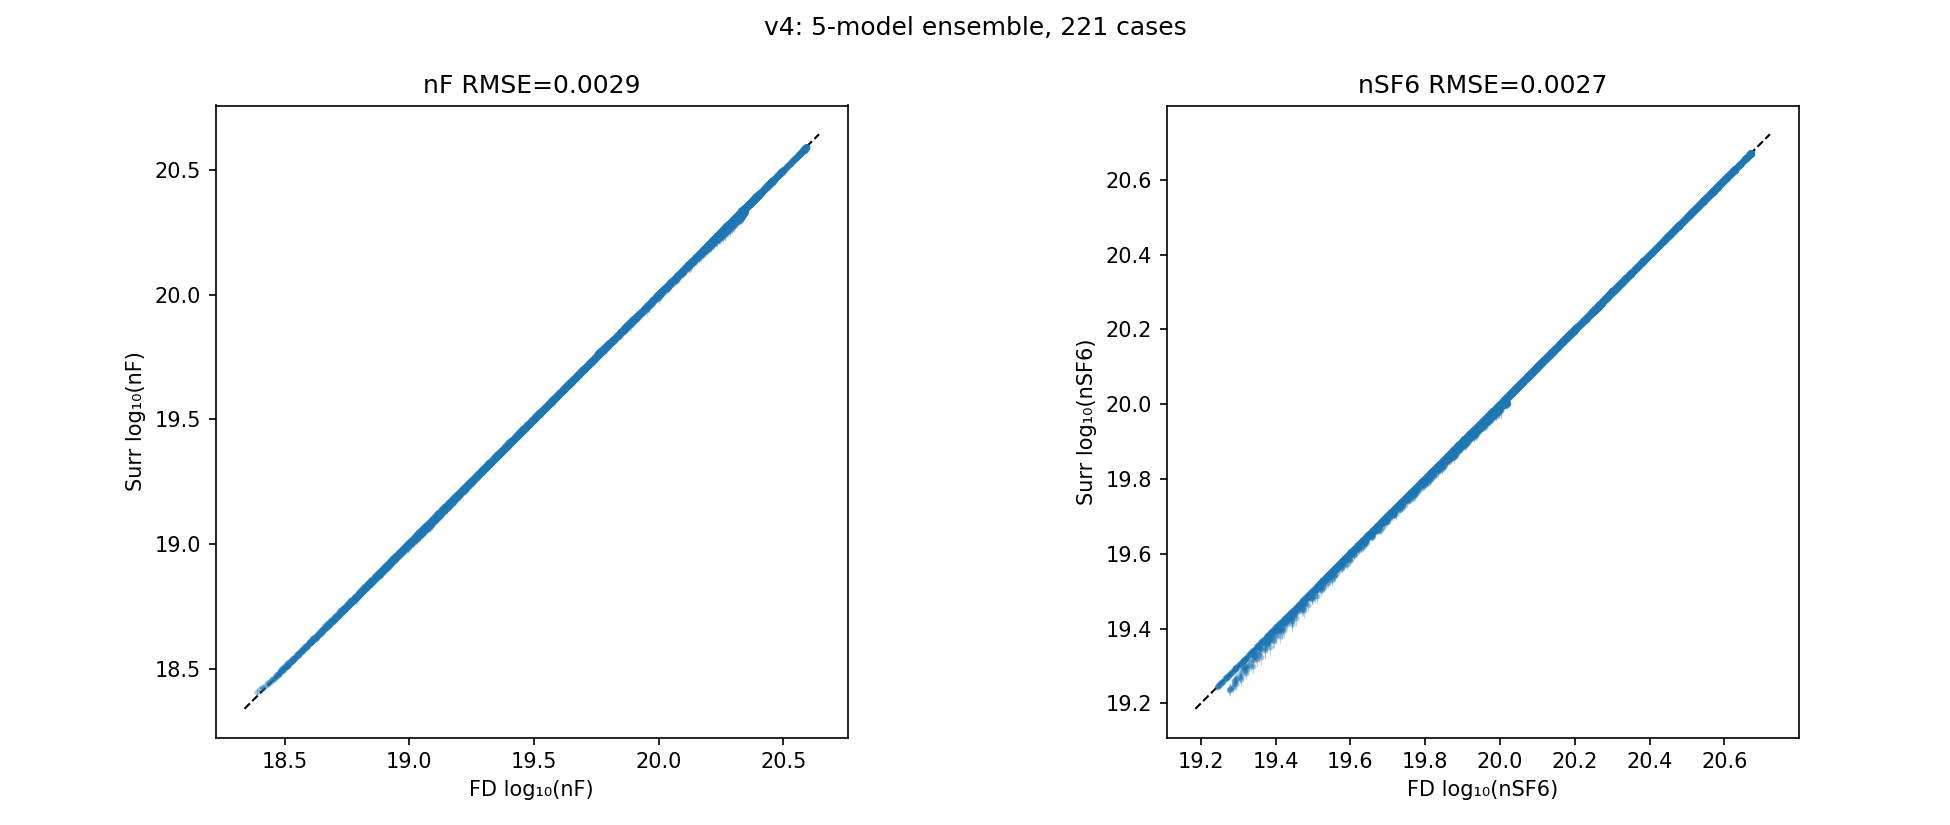
\includegraphics[width=0.6\textwidth]{surrogate_v4_pred_vs_true.png}
  \caption{Predicted vs.\ true log-density for the production
           ensemble on the held-out test set.  Points cluster tightly
           around the identity line across four orders of magnitude.}
  \label{fig:pred_vs_true}
\end{figure}

\subsection{Training Dynamics}

Figure~\ref{fig:loss_curves} shows the training and validation loss
curves.  The cosine-annealing schedule produces periodic loss
reductions; no over-fitting is observed.

\begin{figure}[H]
  \centering
  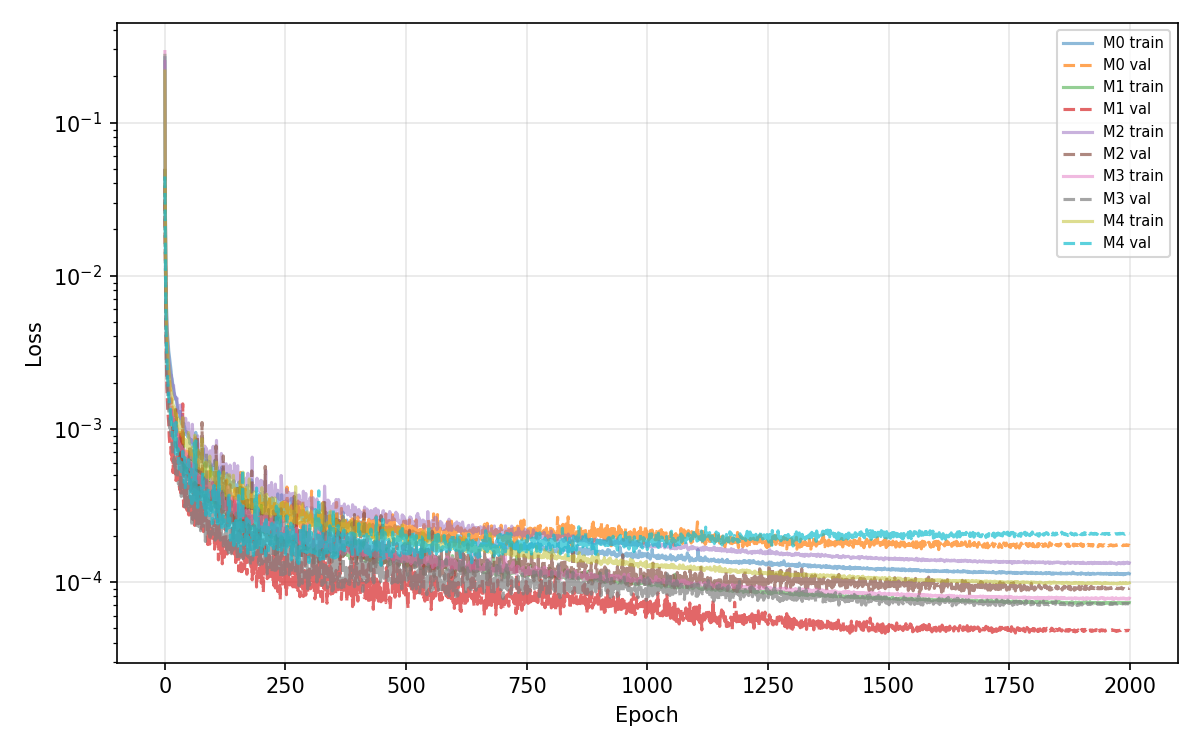
\includegraphics[width=0.6\textwidth]{surrogate_v4_loss_curves.png}
  \caption{Training and validation loss curves for the production
           ensemble.  The cosine-annealing schedule produces periodic
           loss reductions; no over-fitting is observed.}
  \label{fig:loss_curves}
\end{figure}

\subsection{Ensemble Uncertainty}

Figure~\ref{fig:uncertainty} maps the inter-model standard deviation
across the reactor domain.  Uncertainty is largest near the aperture
where density gradients are steepest, providing a physically
meaningful uncertainty estimate.

\begin{figure}[H]
  \centering
  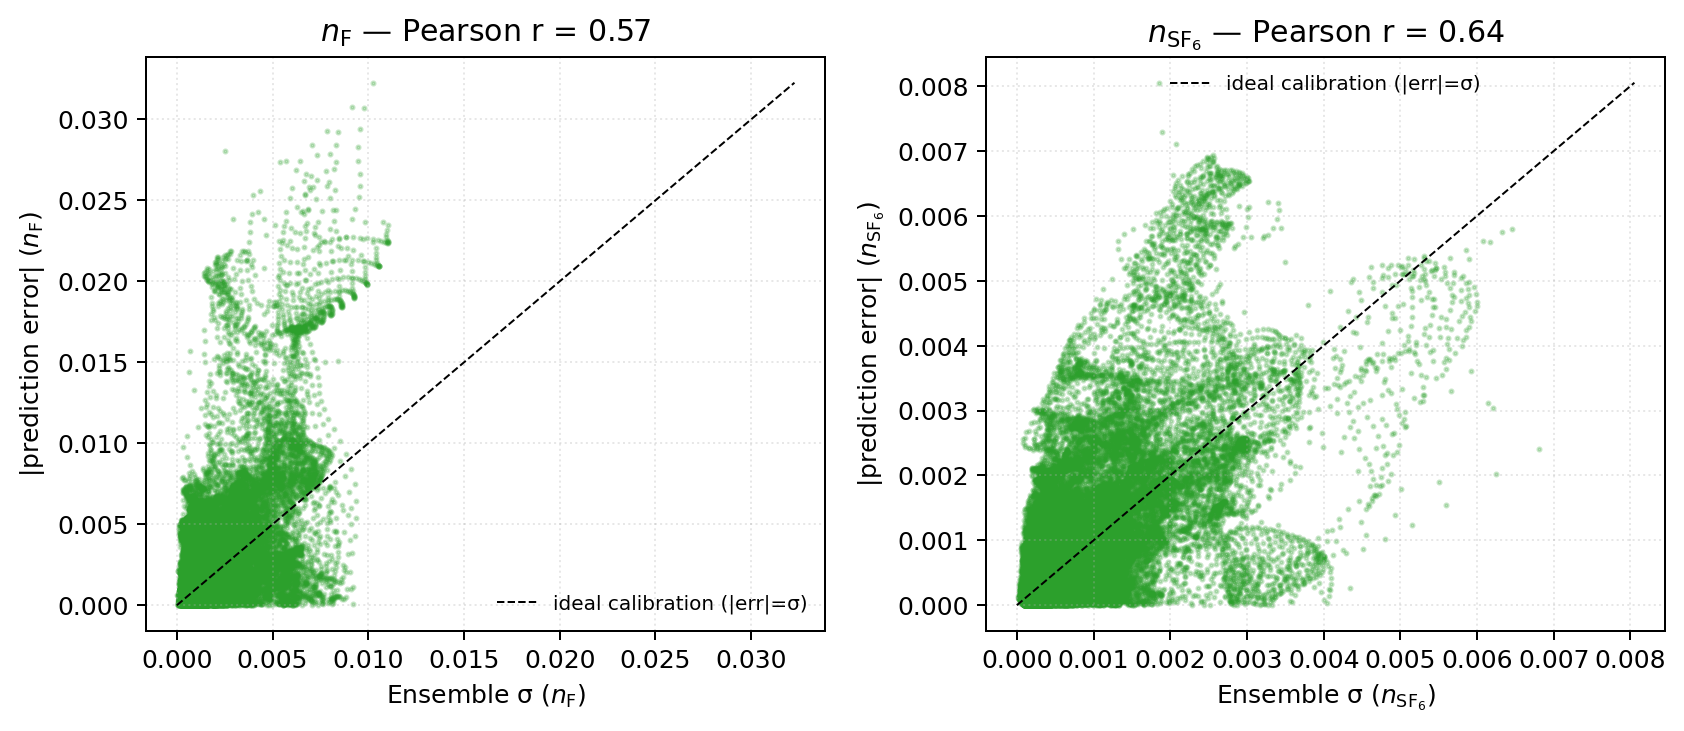
\includegraphics[width=0.6\textwidth]{surrogate_v4_uncertainty.png}
  \caption{Ensemble uncertainty (inter-model standard deviation) as a
           function of spatial position.  Uncertainty is largest near
           the aperture where gradients are steepest.}
  \label{fig:uncertainty}
\end{figure}

\subsection{Spatial Error Distribution}

Figure~\ref{fig:residuals} shows that prediction residuals are
approximately uniform across the domain with no systematic spatial
bias.

\begin{figure}[H]
  \centering
  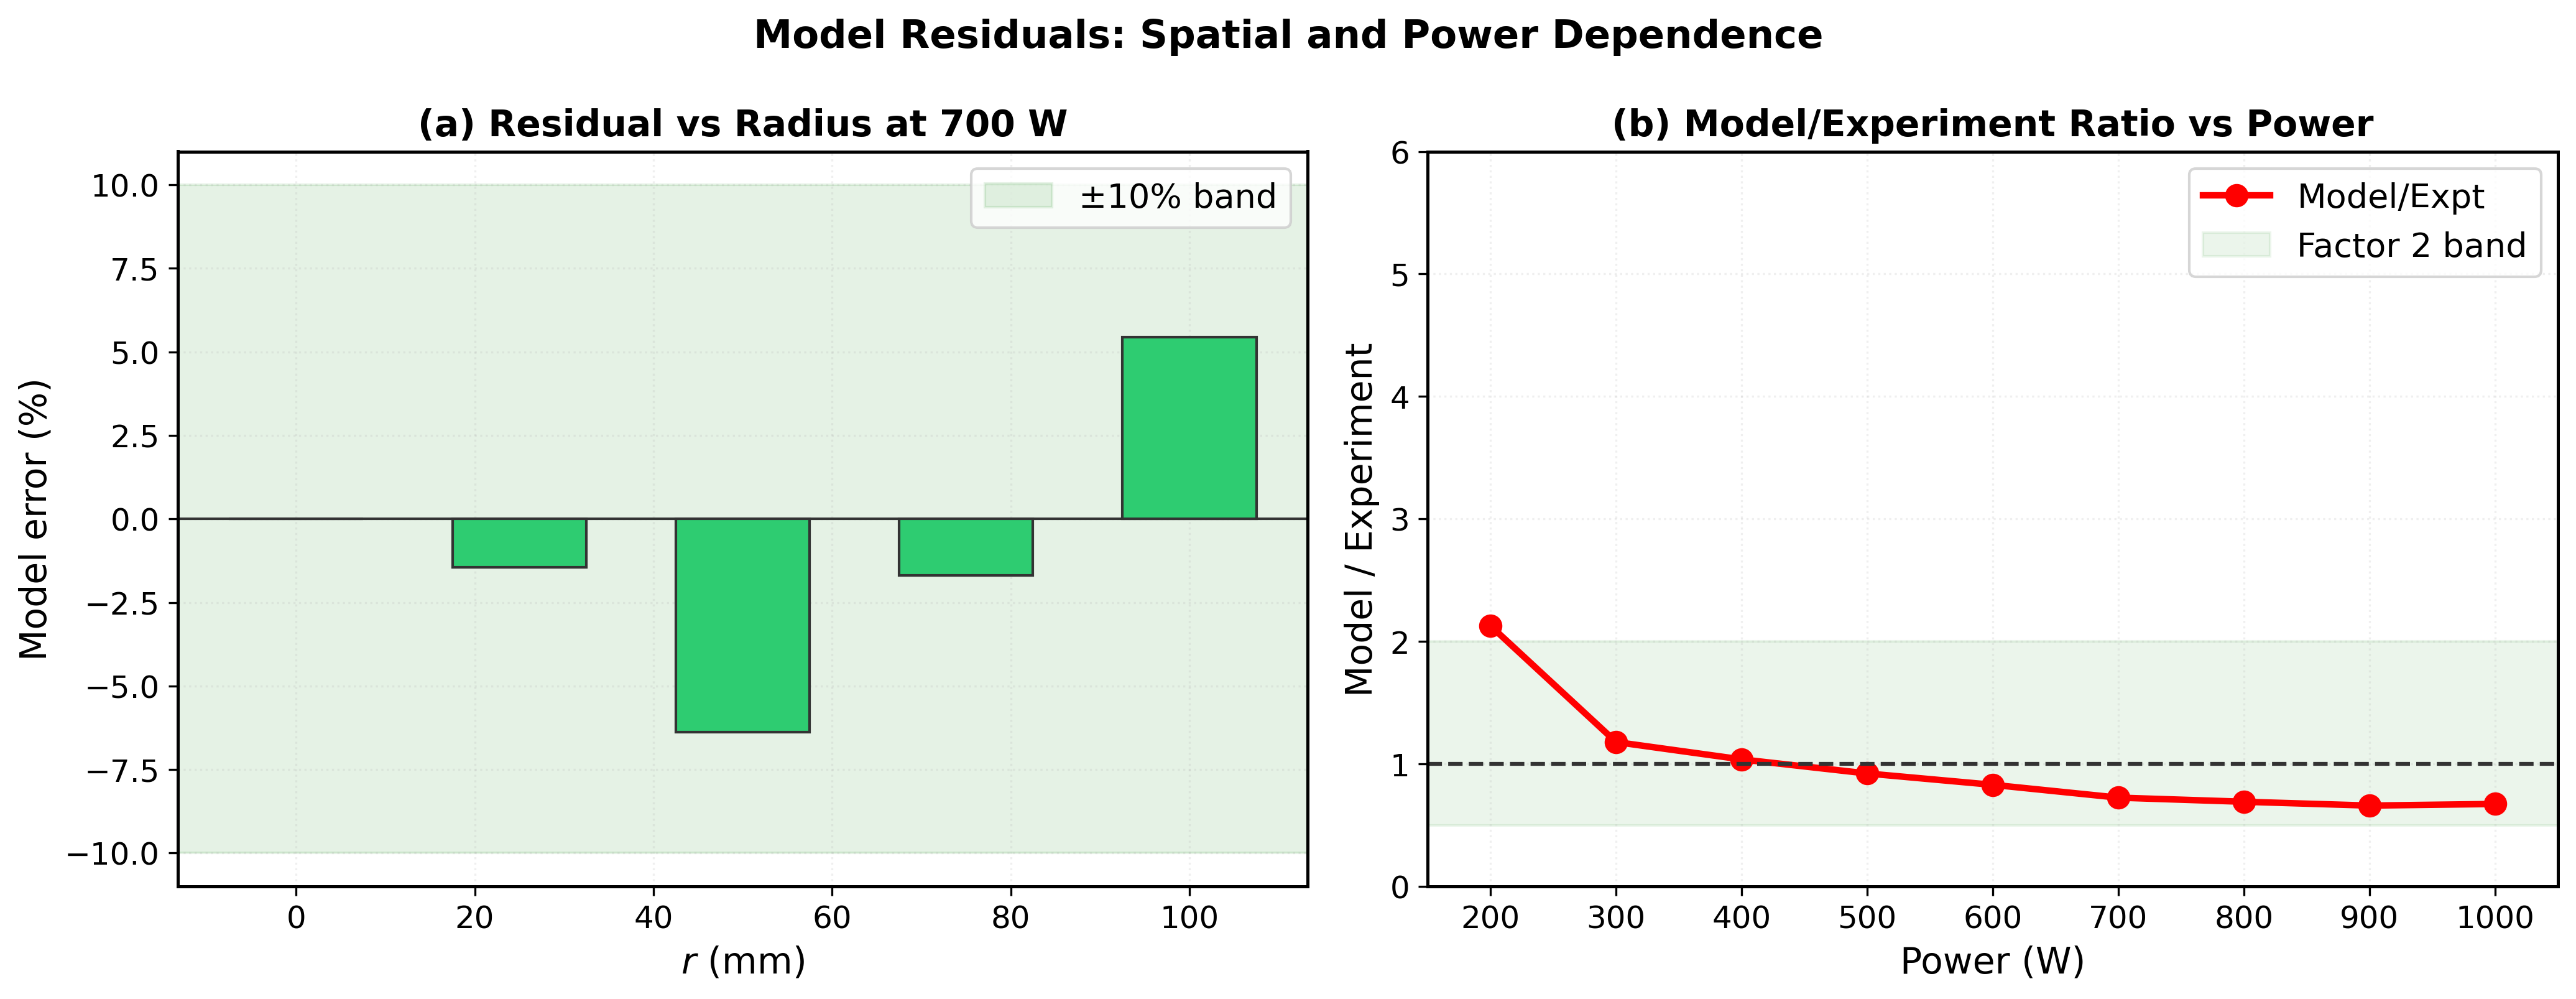
\includegraphics[width=0.6\textwidth]{residuals.png}
  \caption{Spatial distribution of prediction residuals.  The errors
           are approximately uniform across the domain with no
           systematic spatial bias.}
  \label{fig:residuals}
\end{figure}

Table~\ref{tab:spatial_error} confirms this quantitatively by
breaking down the error by reactor region.

\begin{table}[H]
  \centering
  \caption{Normalised nF RMSE by reactor region
           (surrogate\_v4 on legacy dataset).}
  \label{tab:spatial_error}
  \begin{tabular}{lc}
    \toprule
    Region & nF RMSE \\
    \midrule
    ICP source   & 0.00368 \\
    Processing   & 0.00282 \\
    Wafer        & 0.00241 \\
    \bottomrule
  \end{tabular}
\end{table}

The absence of systematic spatial bias confirms that the surrogate
does not favour any particular region of the reactor.

\subsection{Benchmark Profiles}

Figure~\ref{fig:benchmarks} compares surrogate and solver profiles at
selected operating points.  The surrogate faithfully reproduces both
the profile shapes and absolute magnitudes.

\begin{figure}[H]
  \centering
  \begin{subfigure}[t]{0.48\textwidth}
    \centering
    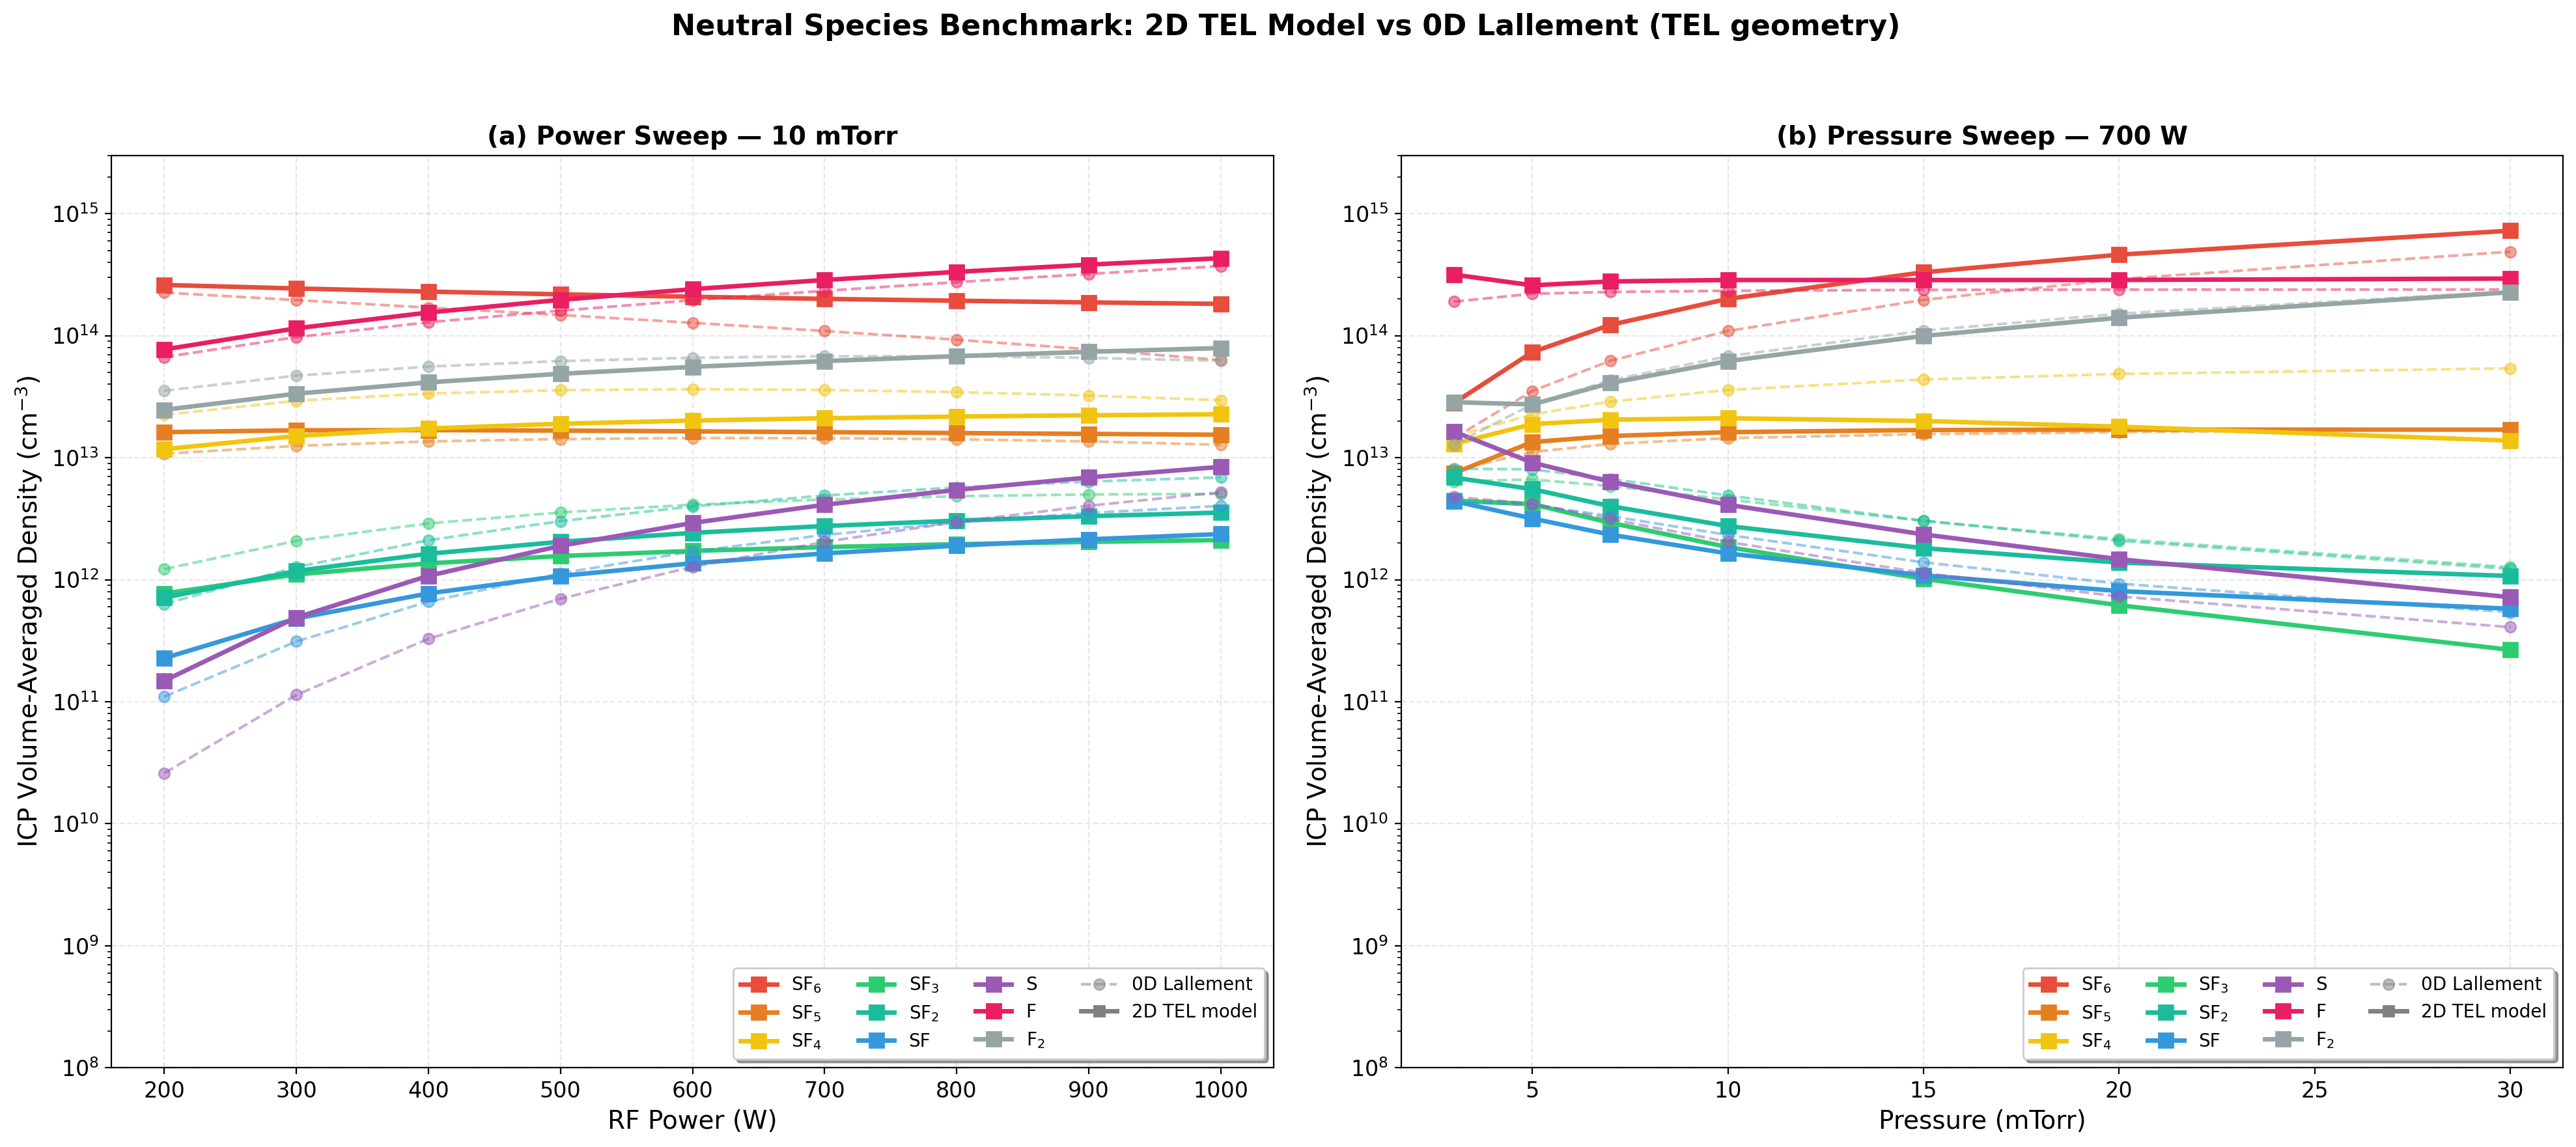
\includegraphics[width=\textwidth]{benchmark_neutrals.png}
    \caption{Neutral species benchmark.}
    \label{fig:bench_neutrals}
  \end{subfigure}
  \hfill
  \begin{subfigure}[t]{0.48\textwidth}
    \centering
    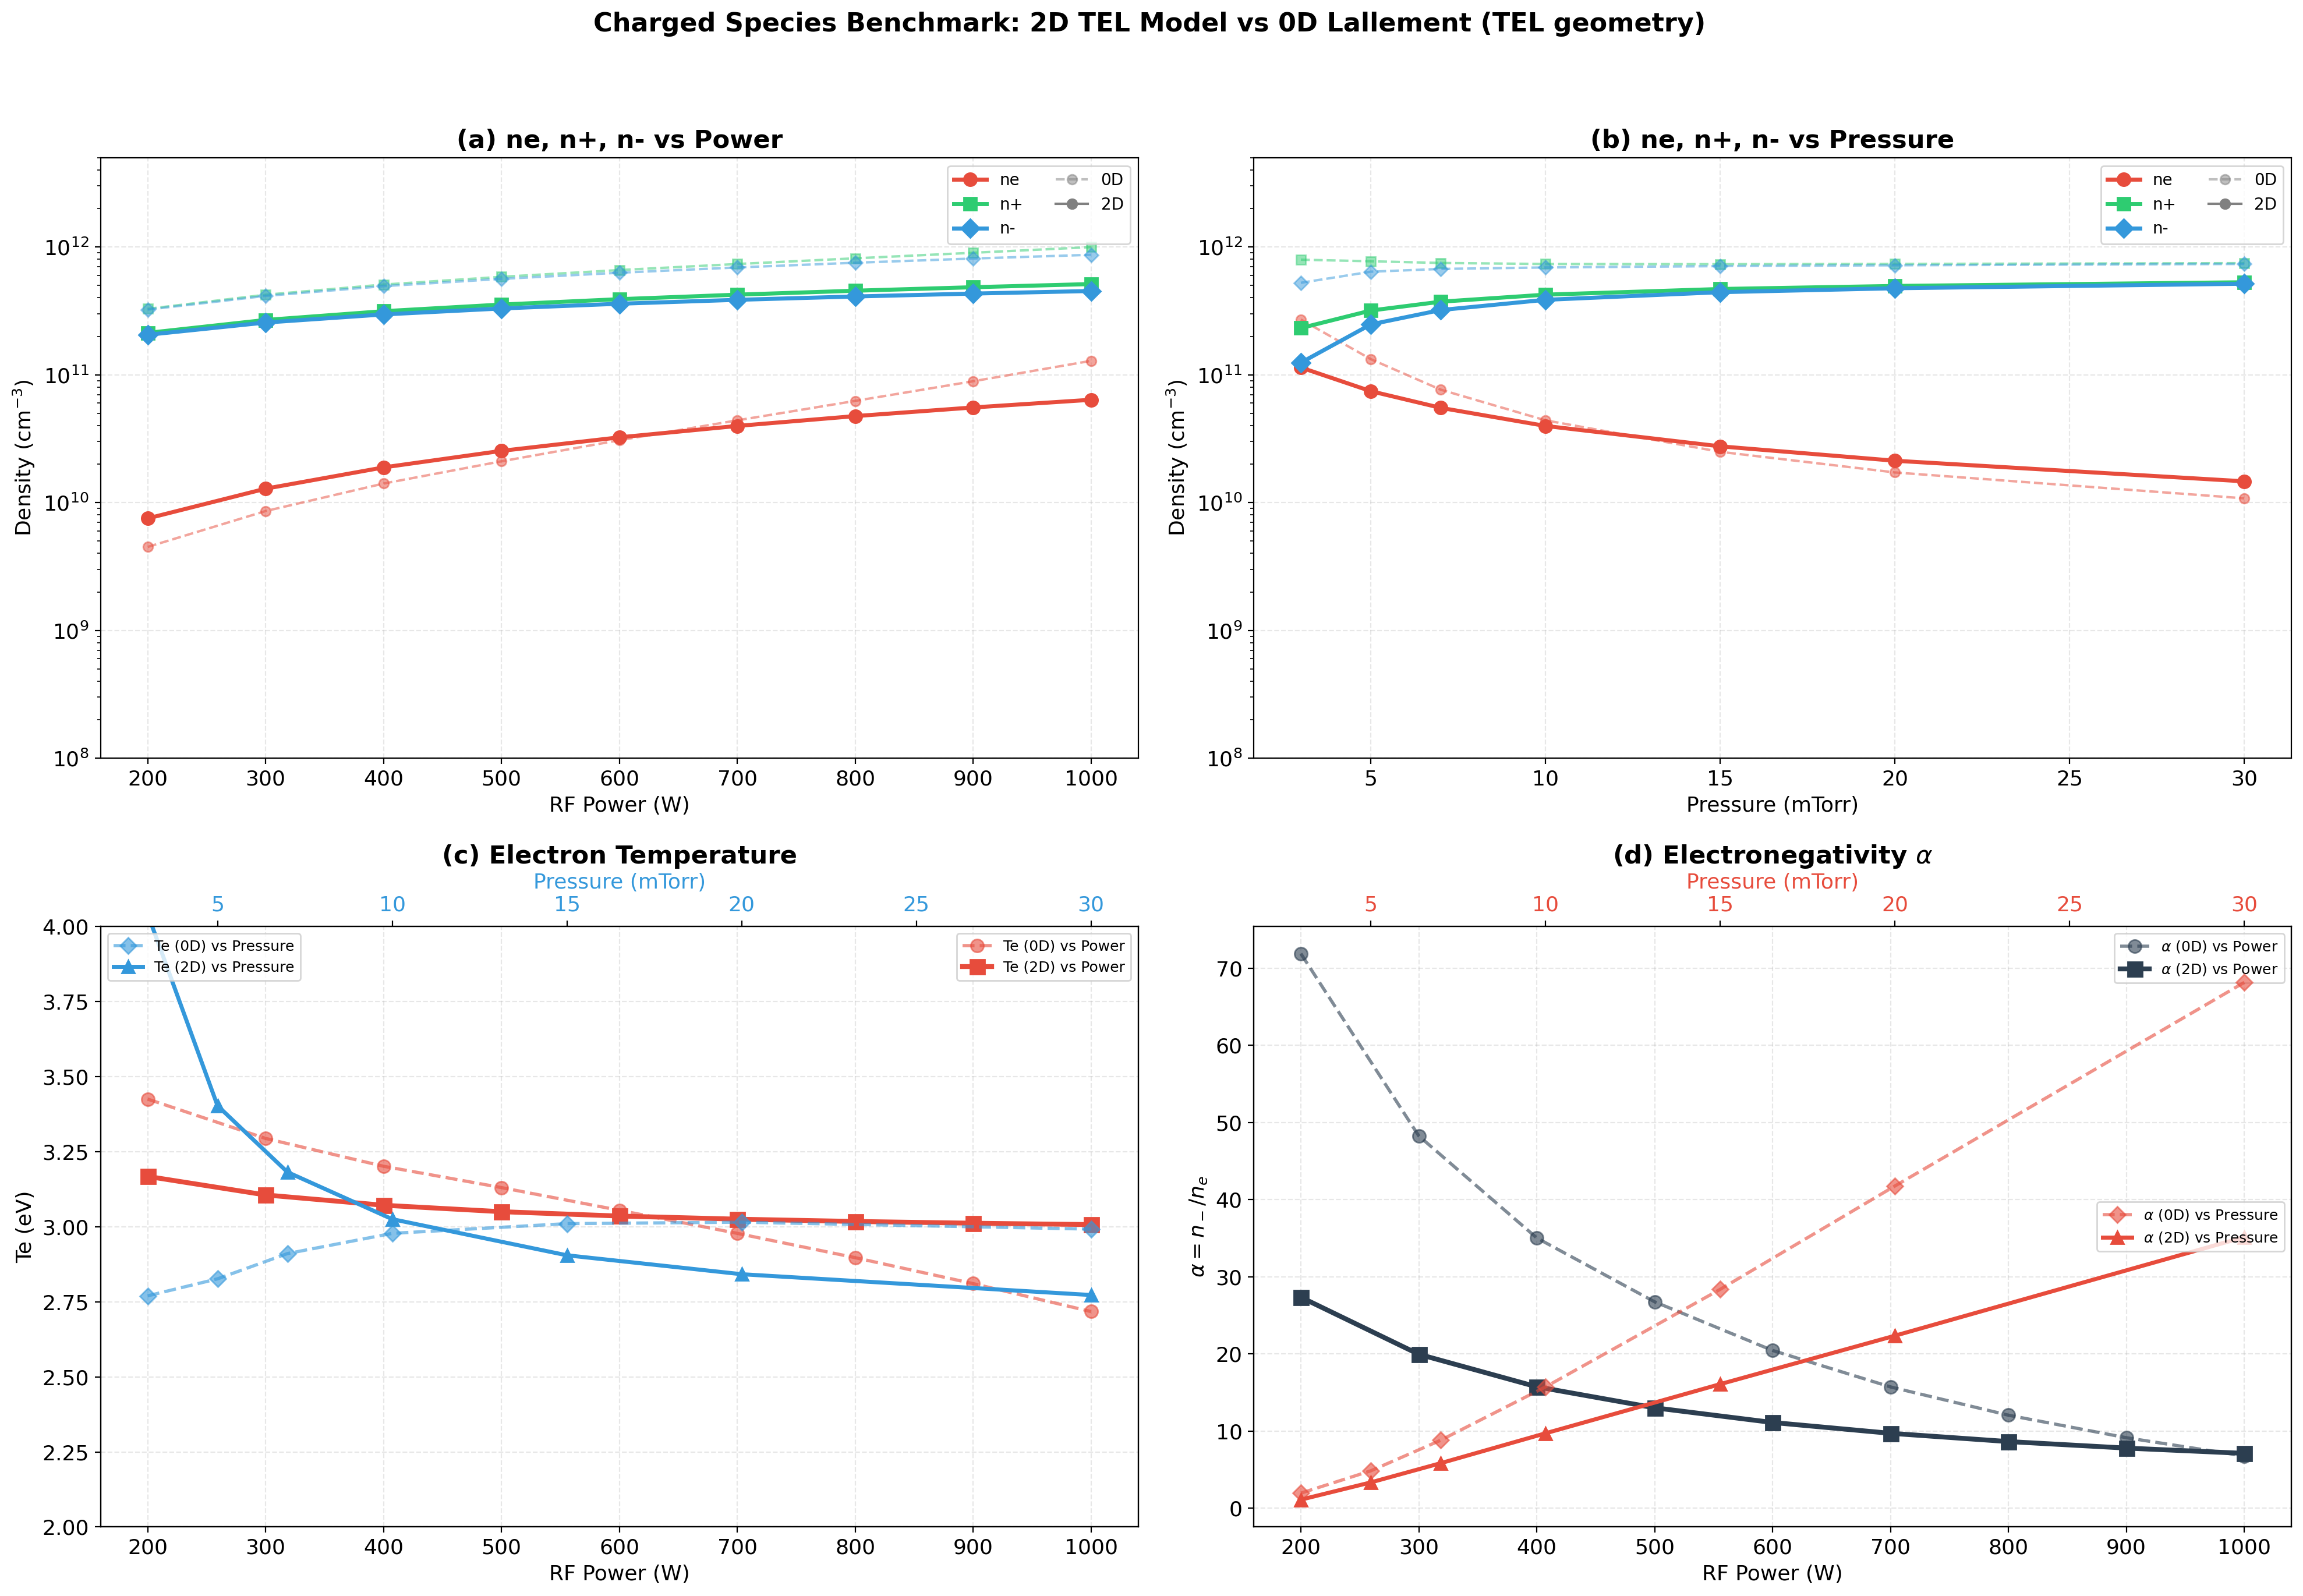
\includegraphics[width=\textwidth]{benchmark_charged.png}
    \caption{Charged species benchmark.}
    \label{fig:bench_charged}
  \end{subfigure}
  \caption{Surrogate vs.\ solver profiles at selected operating points
           for neutral and charged species.  The surrogate faithfully
           reproduces both the profile shapes and absolute magnitudes.}
  \label{fig:benchmarks}
\end{figure}

% ==================================================================
\section{Validation}
\label{sec:validation}

\subsection{Mesh Convergence}

A mesh convergence study was performed at a reference condition of
\SI{700}{\watt} and 10~mTorr.  Table~\ref{tab:mesh} shows relative
errors between the coarse ($30 \times 50$) and fine ($50 \times 80$)
meshes.

\begin{table}[H]
  \centering
  \caption{Mesh convergence: relative error between $30 \times 50$
           and $50 \times 80$ grids at \SI{700}{\watt}, 10~mTorr.}
  \label{tab:mesh}
  \begin{tabular}{lc}
    \toprule
    Species & Relative error (\%) \\
    \midrule
    $n_{\text{F}}$               & 1.86 \\
    $n_{\text{SF}_6}$            & 2.30 \\
    $n_e$                        & 4.89 \\
    \bottomrule
  \end{tabular}
\end{table}

The $\sim$2\% mesh error for the surrogate target species (F and
SF\textsubscript{6}) is well below the surrogate RMSE and the
systematic modelling uncertainties, confirming that the coarser mesh
is adequate for training-data generation.

\subsection{Literature Validation: F Density}

Figure~\ref{fig:lit_F_power} compares the predicted F density versus
RF power to the measurements of \citet{mettler2020}.  Both the legacy
and LXCat solvers exhibit a \textbf{36\% mean relative error}
(systematic over-prediction at all powers), attributed to differences
in reactor geometry, wall recombination coefficients, and the
simplified 2D axisymmetric assumption.

\begin{figure}[H]
  \centering
  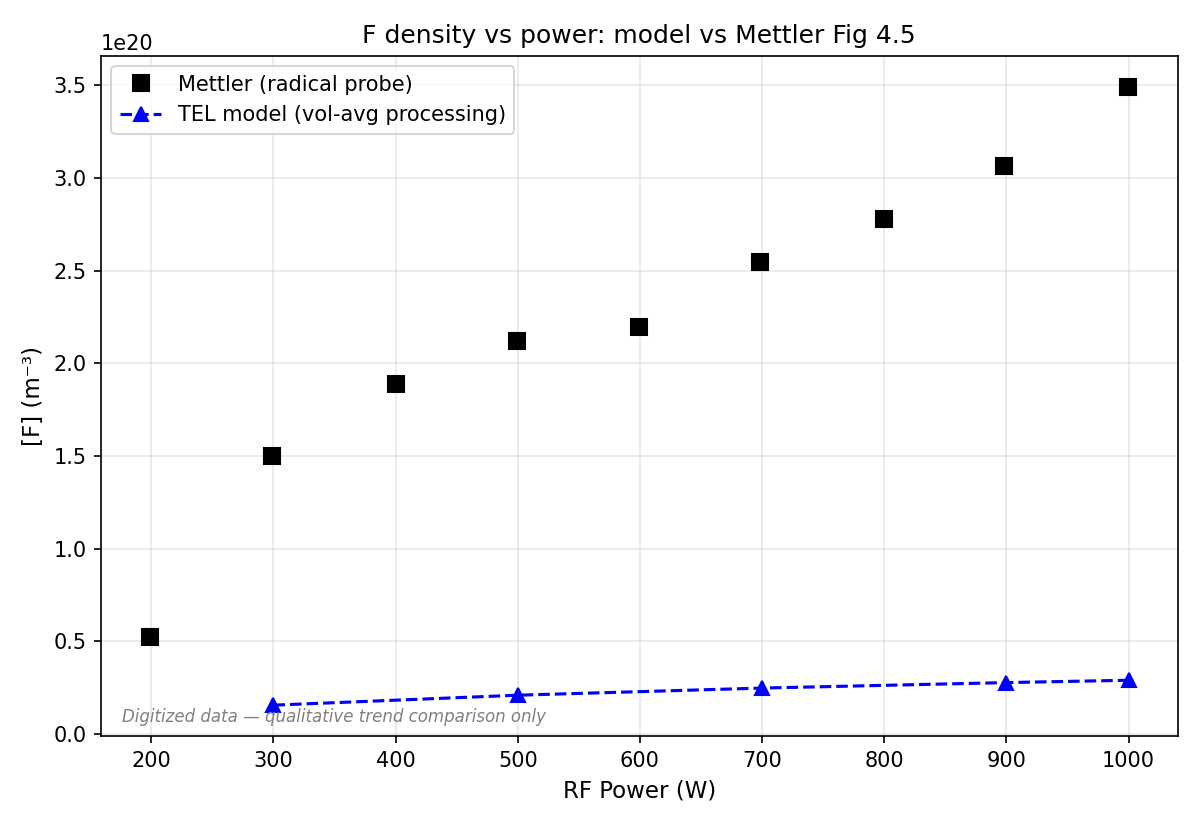
\includegraphics[width=0.6\textwidth]{lit_F_vs_power.png}
  \caption{Fluorine atom density as a function of RF power.
           Simulation results (legacy and LXCat solvers) are compared
           to the measurements of \citet{mettler2020}.  Both solvers
           show a 36\% mean relative error.}
  \label{fig:lit_F_power}
\end{figure}

\subsection{Literature Validation: Electron Temperature}

Figure~\ref{fig:lit_Te} compares $T_e$ versus RF power to
\citet{lallement2009}.  The legacy solver agrees well (RMSE =
\SI{0.17}{\electronvolt}, 5\%), while the LXCat solver significantly
overpredicts $T_e$ (RMSE = \SI{1.68}{\electronvolt}, 58\%).  This
confirms the cross-section-driven $T_e$ shift discussed in
Section~\ref{sec:lxcat}.

\begin{figure}[H]
  \centering
  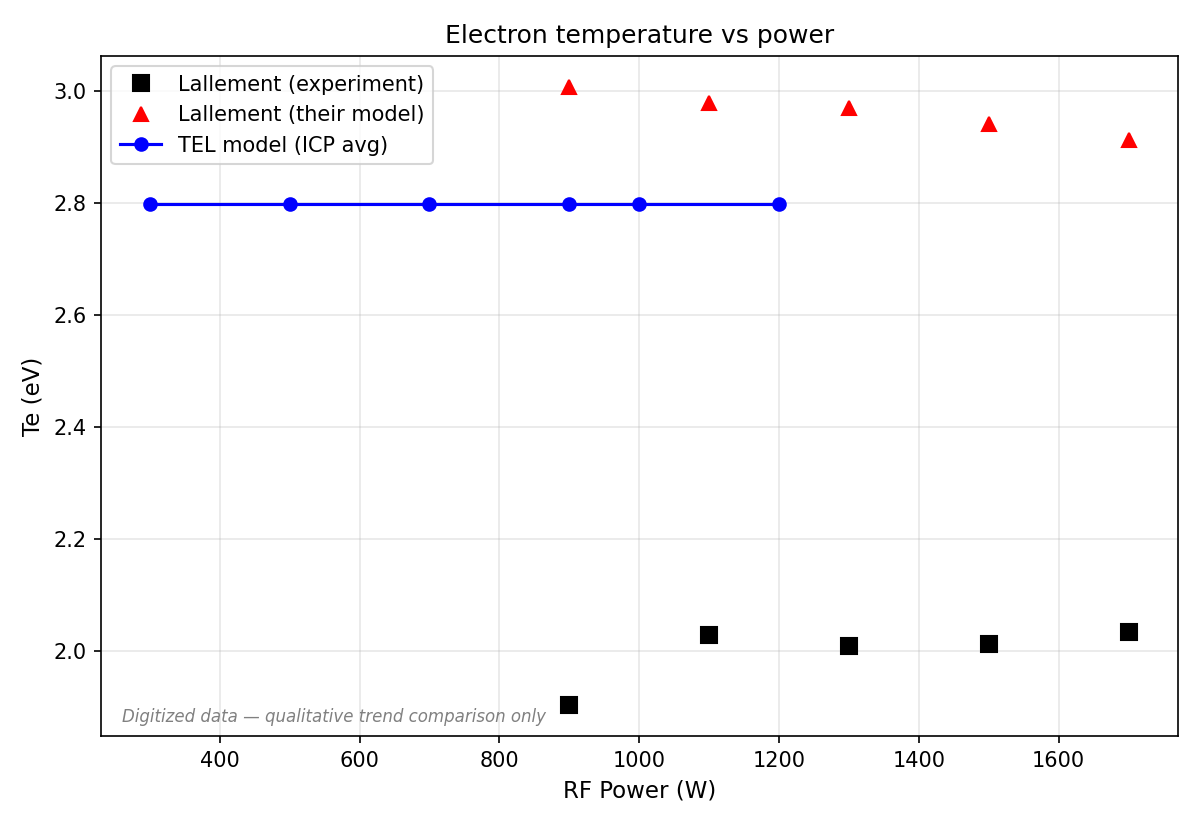
\includegraphics[width=0.6\textwidth]{lit_Te_vs_power.png}
  \caption{Electron temperature vs.\ RF power compared to
           \citet{lallement2009}.  The legacy solver agrees well
           (5\%), while the LXCat solver overpredicts by 58\%.}
  \label{fig:lit_Te}
\end{figure}

\subsection{Additional Literature Comparisons}

Figure~\ref{fig:lit_other} provides further validation points:
radial F profiles and electron density scaling with power.

\begin{figure}[H]
  \centering
  \begin{subfigure}[t]{0.48\textwidth}
    \centering
    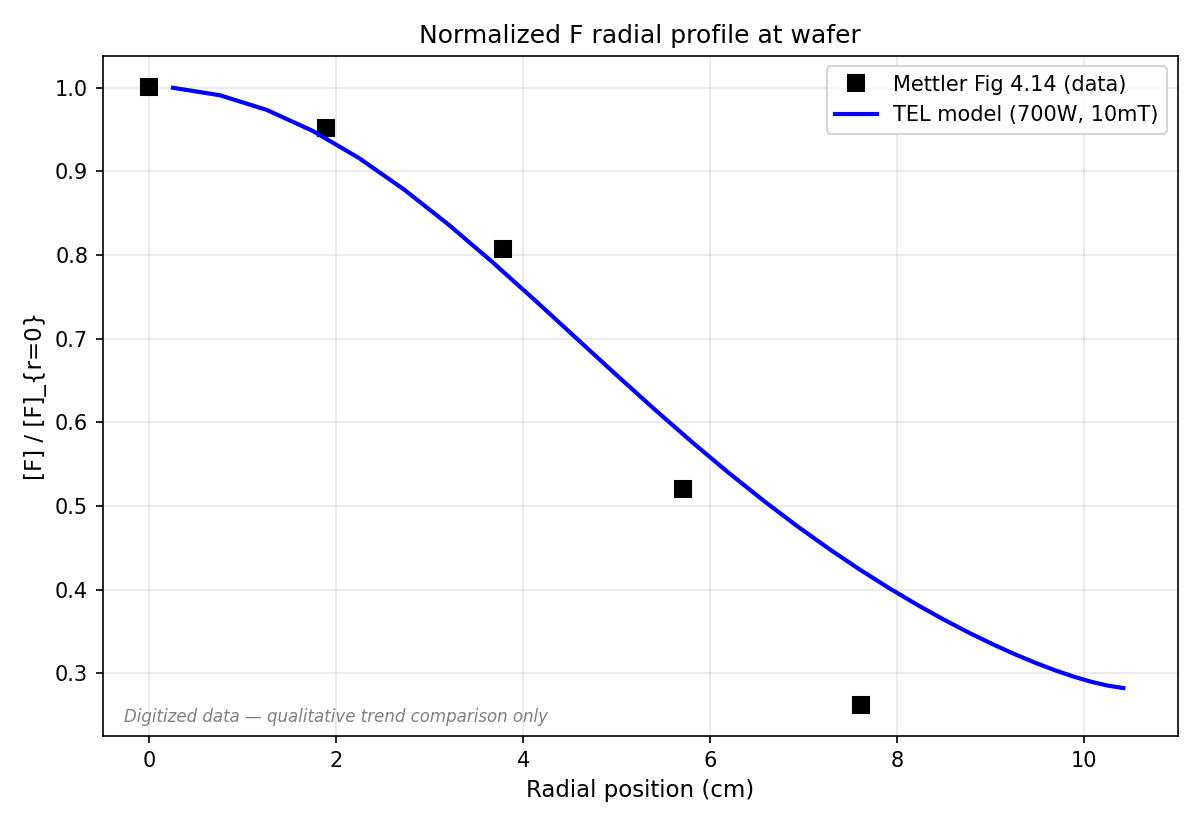
\includegraphics[width=\textwidth]{lit_F_radial_profile.png}
    \caption{Radial F profile vs.\ literature.}
    \label{fig:lit_F_radial}
  \end{subfigure}
  \hfill
  \begin{subfigure}[t]{0.48\textwidth}
    \centering
    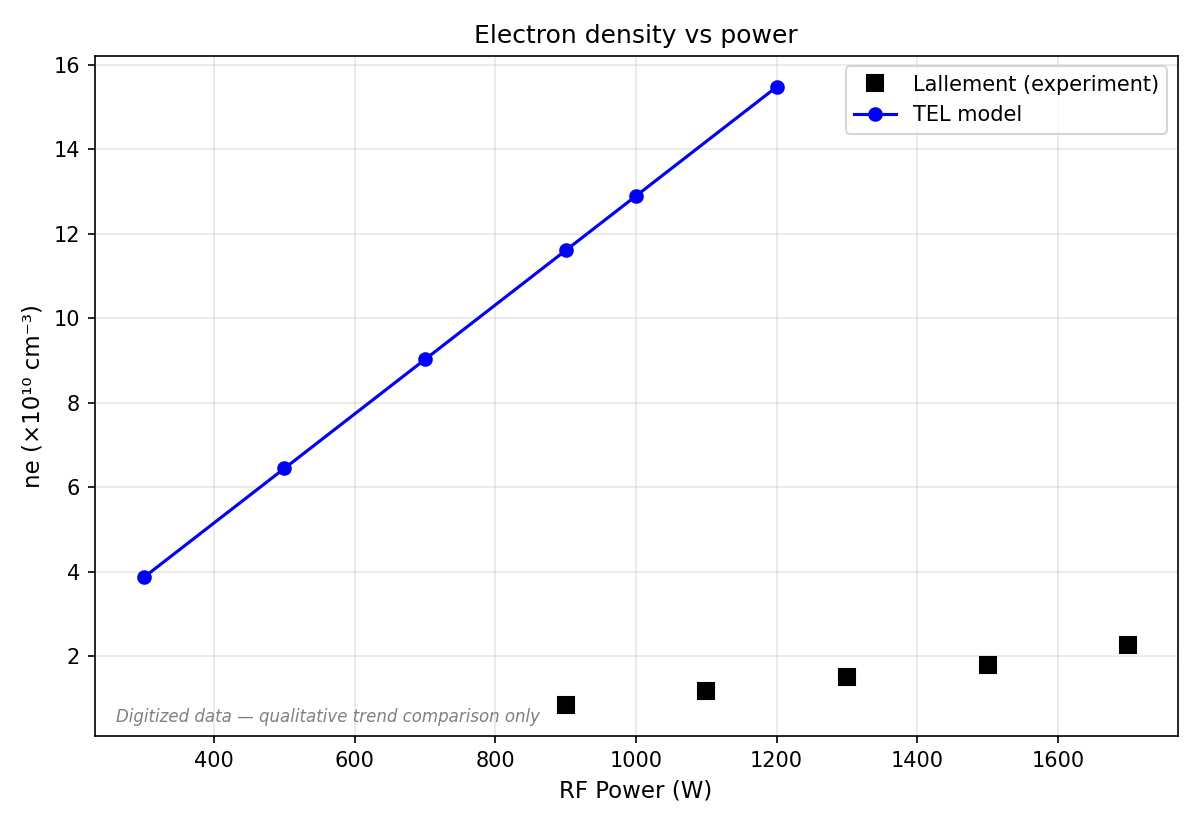
\includegraphics[width=\textwidth]{lit_ne_vs_power.png}
    \caption{Electron density vs.\ power.}
    \label{fig:lit_ne}
  \end{subfigure}
  \caption{Additional literature comparisons showing radial F profiles
           and electron density scaling with power.}
  \label{fig:lit_other}
\end{figure}

\subsection{Absolute Validation Summary}

Figure~\ref{fig:abs_validation} summarises the absolute validation
metrics across all measured quantities.  The model captures trends
correctly but has systematic offsets in absolute values.

\begin{figure}[H]
  \centering
  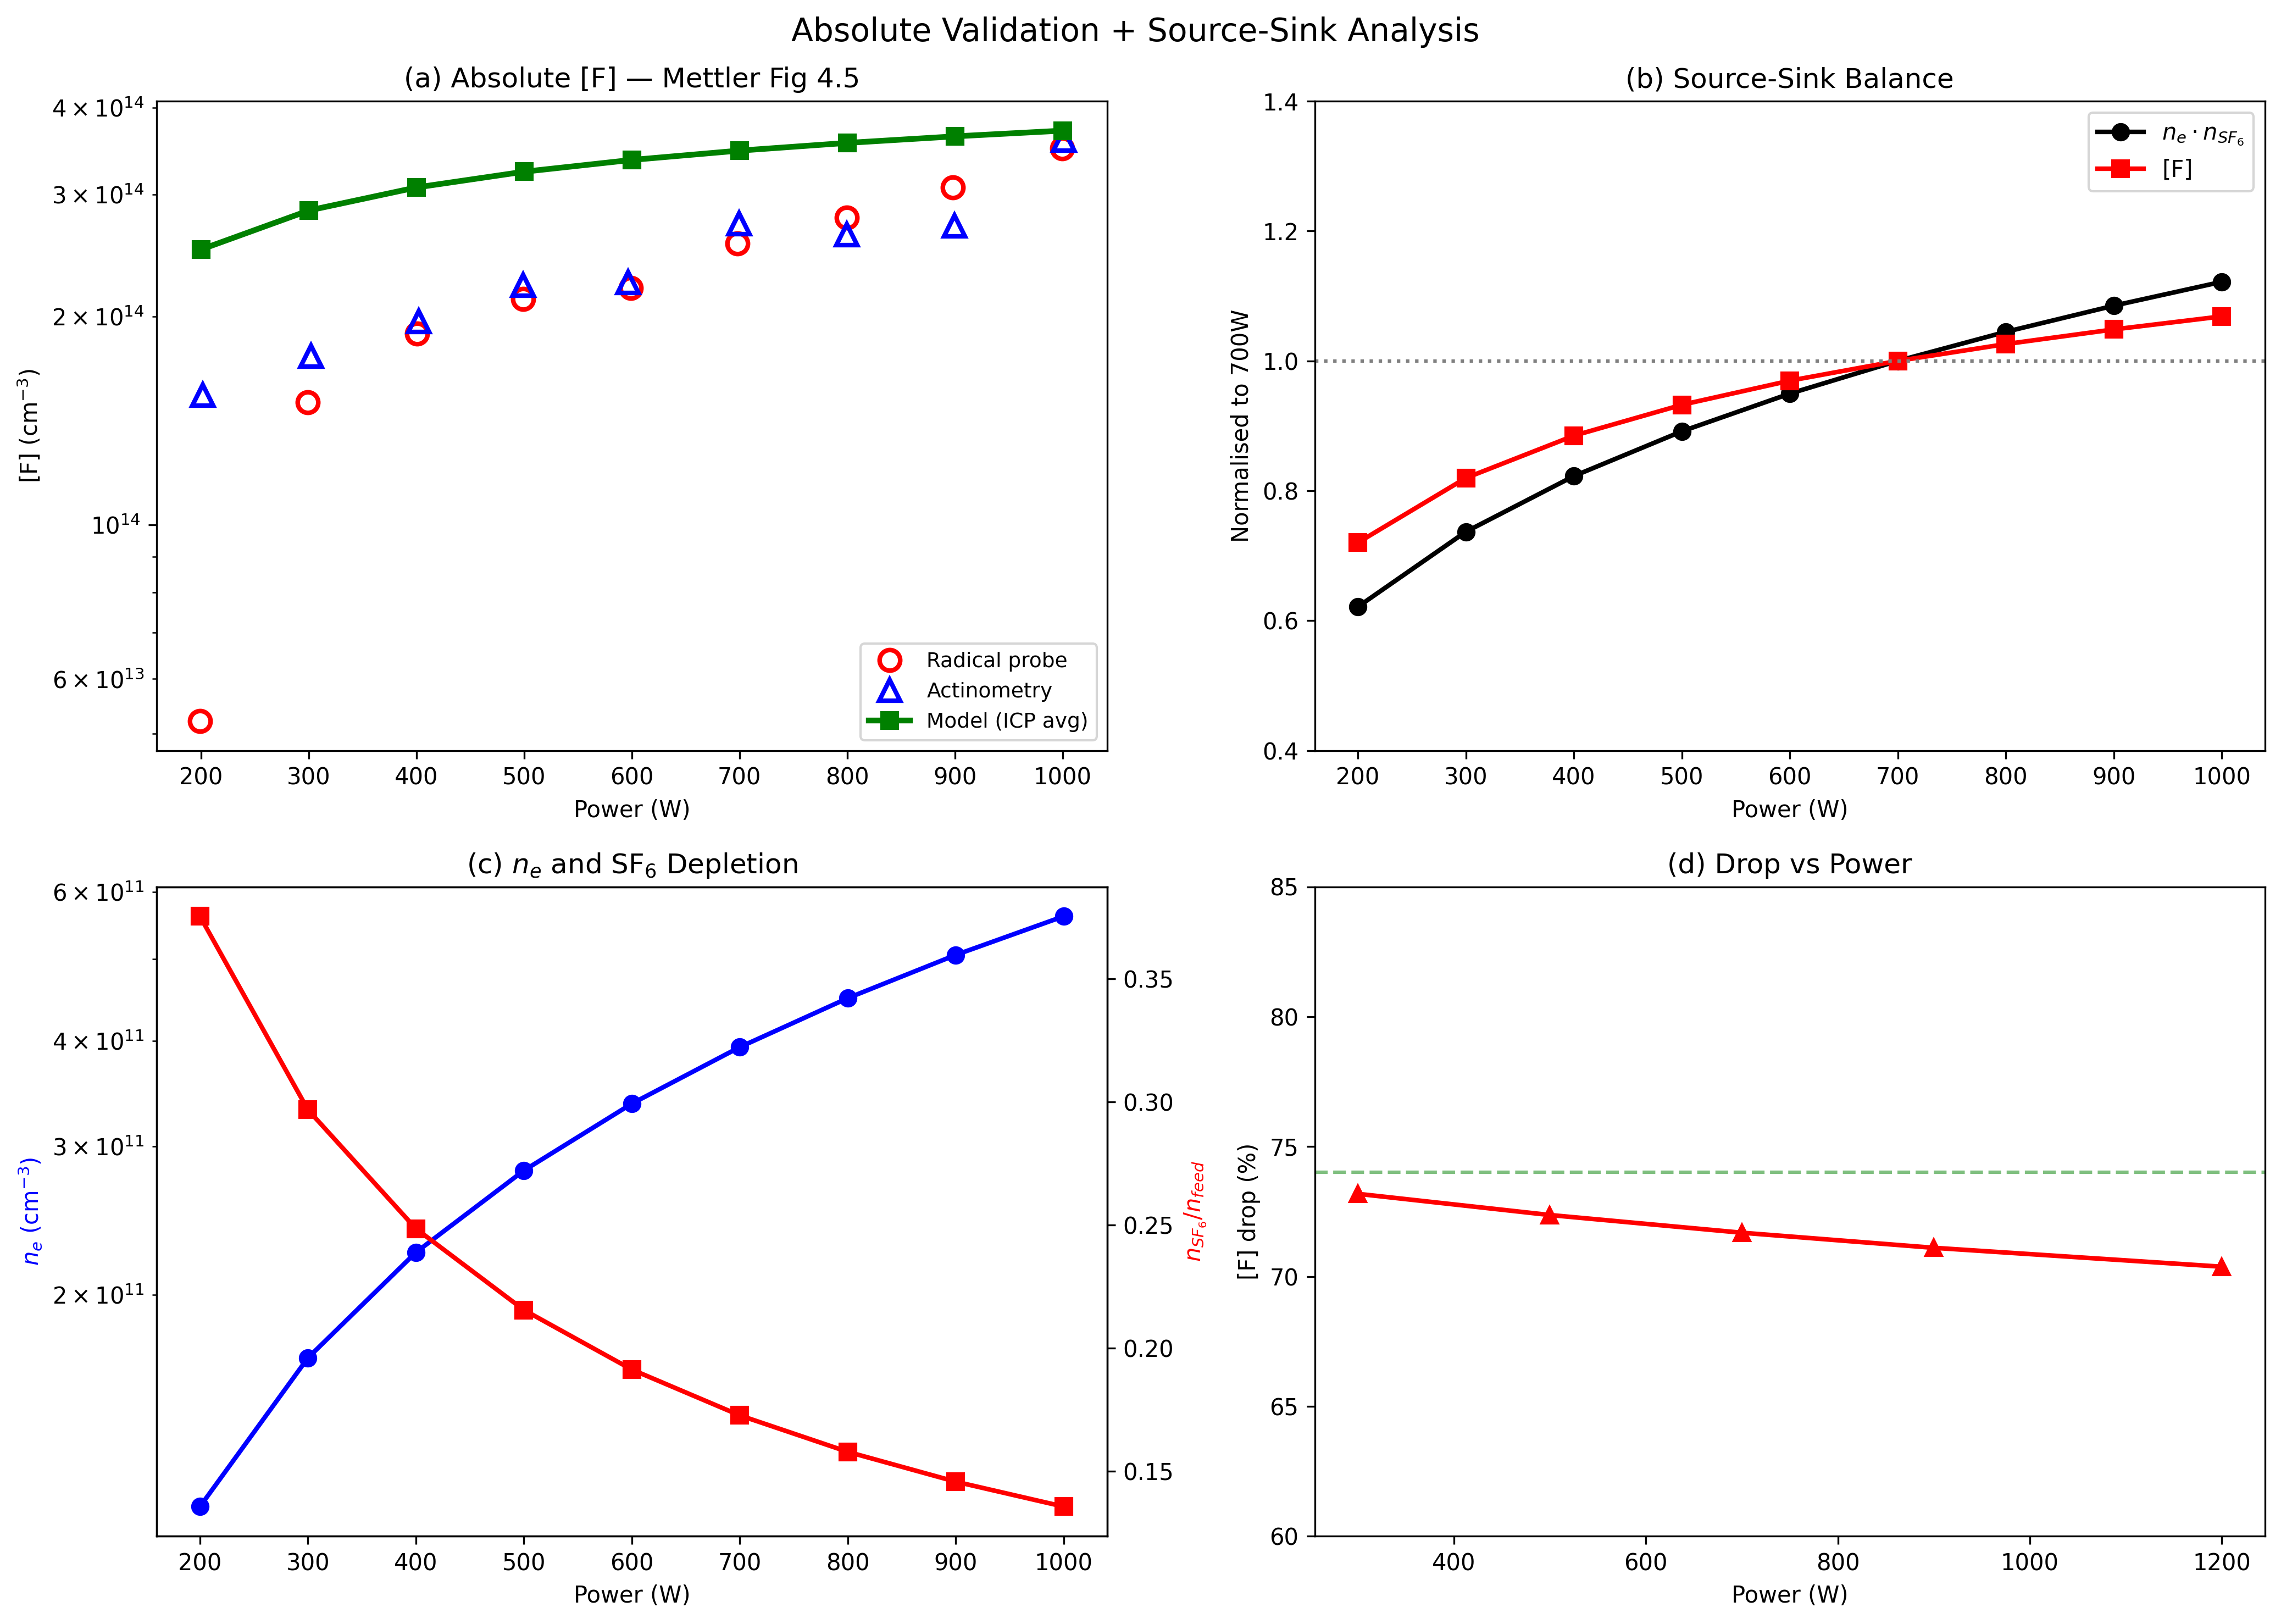
\includegraphics[width=0.65\textwidth]{absolute_validation.png}
  \caption{Summary of absolute validation metrics across all
           measured quantities.  The model captures trends
           correctly but has systematic offsets in absolute values.}
  \label{fig:abs_validation}
\end{figure}

\subsection{ML Baselines}

Table~\ref{tab:baselines} compares the MLP ensemble to classical
machine-learning baselines.

\begin{table}[H]
  \centering
  \caption{Comparison of surrogate approaches (nF RMSE).}
  \label{tab:baselines}
  \begin{tabular}{lc}
    \toprule
    Method & nF RMSE \\
    \midrule
    Polynomial (degree 3)          & 0.051  \\
    Polynomial (degree 4)          & 0.039  \\
    Gaussian Process (3000 points) & 0.006  \\
    MLP ensemble (this work)       & 0.0015 \\
    \bottomrule
  \end{tabular}
\end{table}

The MLP ensemble outperforms all baselines by wide margins.
The Gaussian process (nF RMSE = 0.006) is competitive but limited to
small training sets due to cubic scaling.  Even degree-4 polynomials
(nF RMSE = 0.039) are $26\times$ worse than the production ensemble.

\subsection{Speedup}

Table~\ref{tab:speedup} summarises the wall-clock speedup.

\begin{table}[H]
  \centering
  \caption{Solver vs.\ surrogate wall-clock times.}
  \label{tab:speedup}
  \begin{tabular}{lccc}
    \toprule
    Solver & Mean time & Surrogate time & Speedup \\
    \midrule
    Legacy & \SI{7.76}{\second} & \SI{14.6}{\milli\second}
           & $531\times$ \\
    LXCat  & \SI{14.4}{\second} & \SI{16.5}{\milli\second}
           & $874\times$ \\
    \bottomrule
  \end{tabular}
\end{table}

The surrogate achieves a $531\times$ speedup over the legacy solver
and an $874\times$ speedup over the more expensive LXCat solver, with
both evaluations completing in under \SI{17}{\milli\second}.

% ==================================================================
\section{Parameter Sensitivity and Sweep Results}
\label{sec:sweeps}

To contextualise the surrogate's operating range, we present the
solver's parameter sweeps (Figures~\ref{fig:sweeps}--\ref{fig:sensitivity}).
These also serve as test cases for the surrogate.

\begin{figure}[H]
  \centering
  \begin{subfigure}[t]{0.48\textwidth}
    \centering
    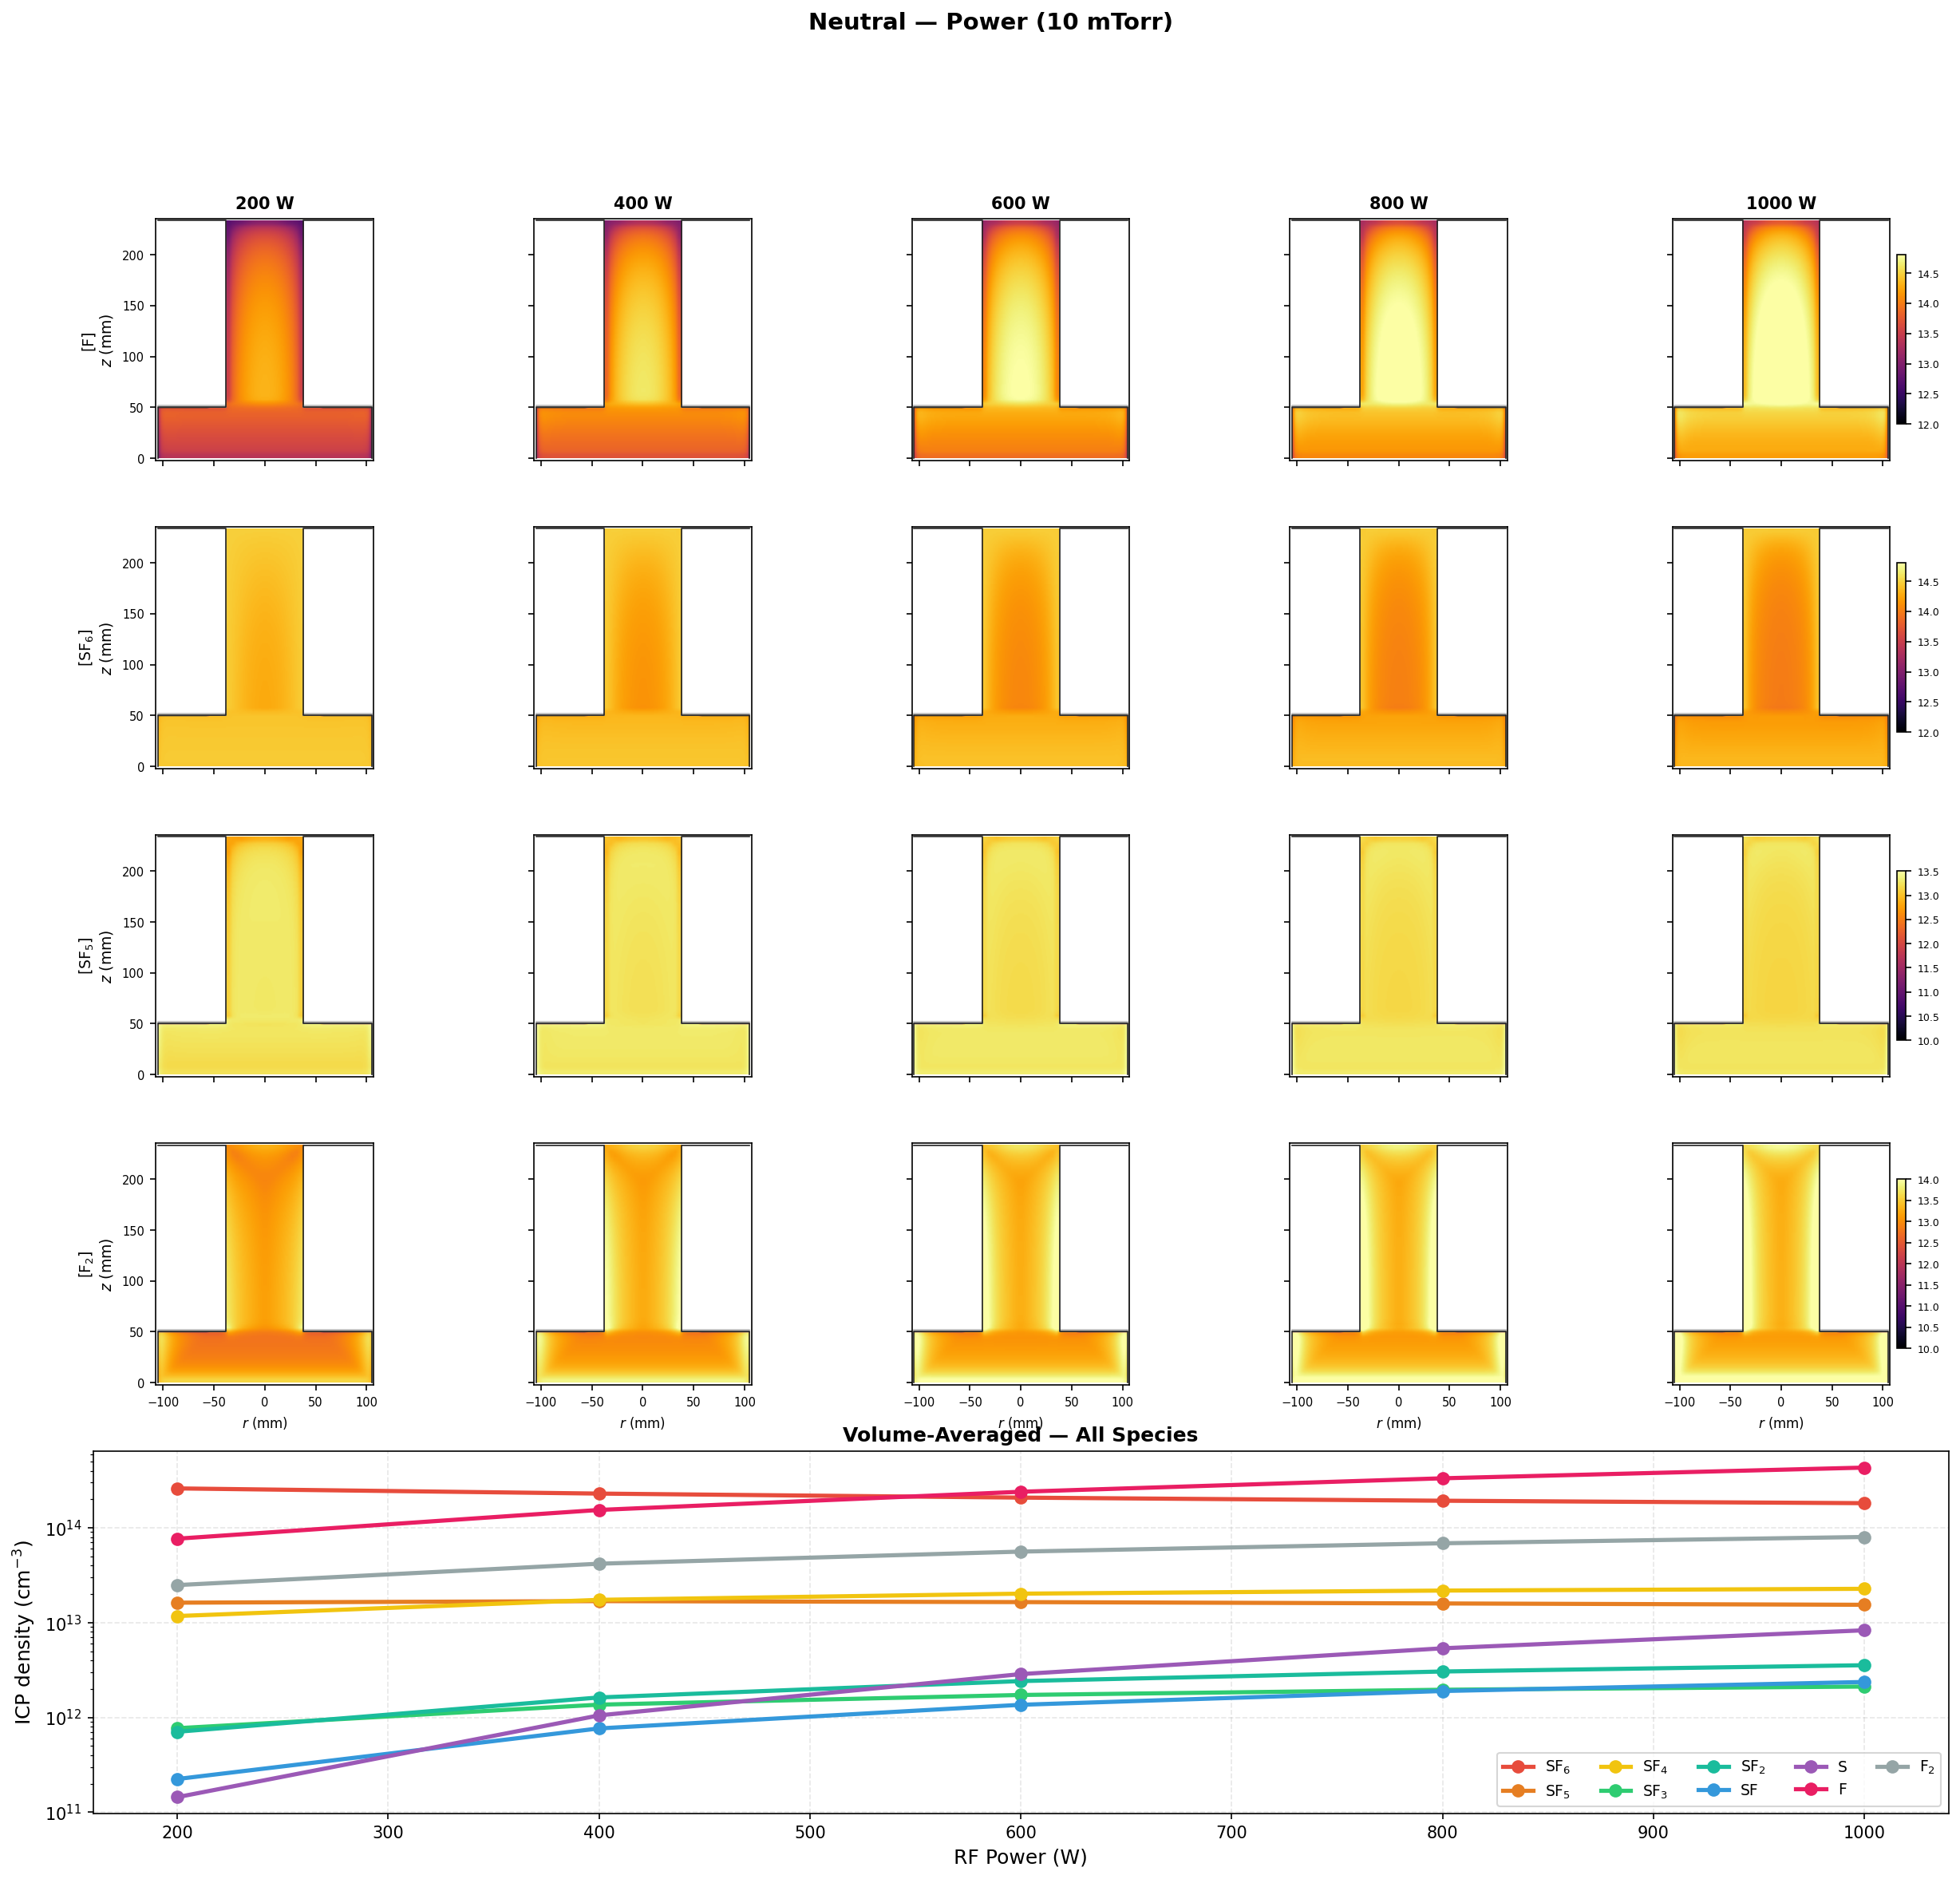
\includegraphics[width=\textwidth]{neutral_power_2D.png}
    \caption{Neutral density vs.\ RF power.}
    \label{fig:neutral_power}
  \end{subfigure}
  \hfill
  \begin{subfigure}[t]{0.48\textwidth}
    \centering
    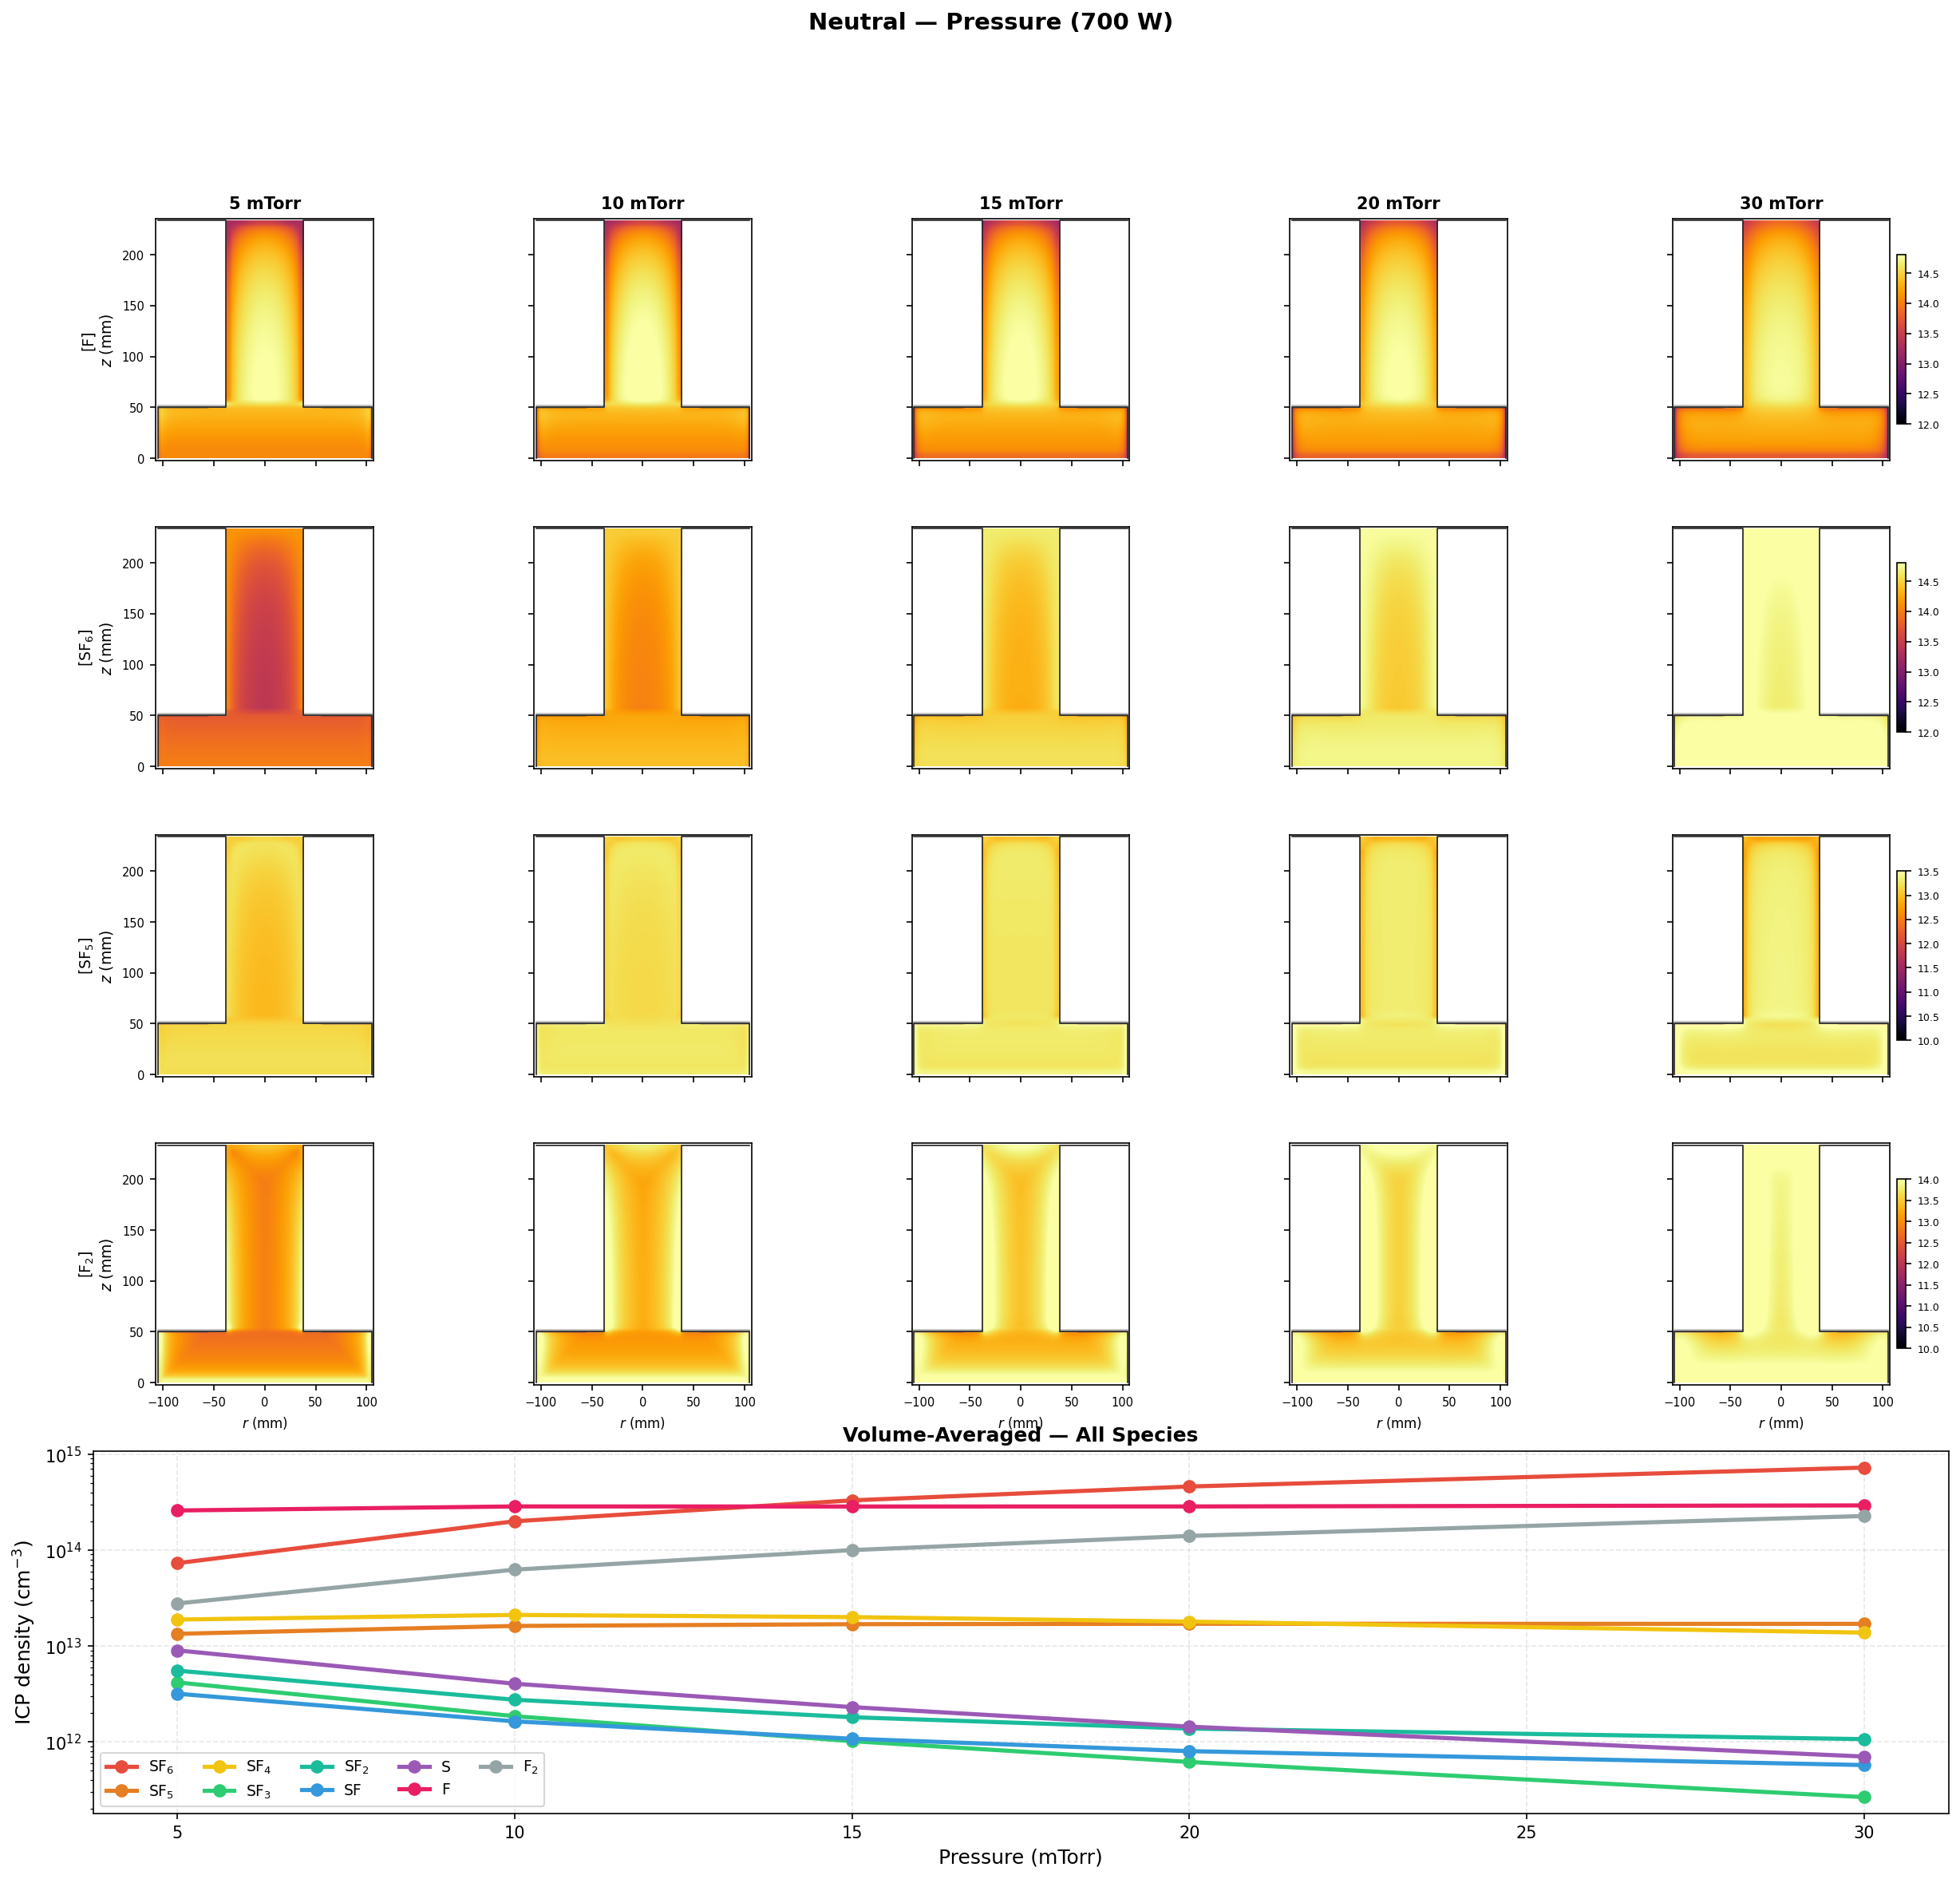
\includegraphics[width=\textwidth]{neutral_pressure_2D.png}
    \caption{Neutral density vs.\ pressure.}
    \label{fig:neutral_pressure}
  \end{subfigure}
  \\[6pt]
  \begin{subfigure}[t]{0.48\textwidth}
    \centering
    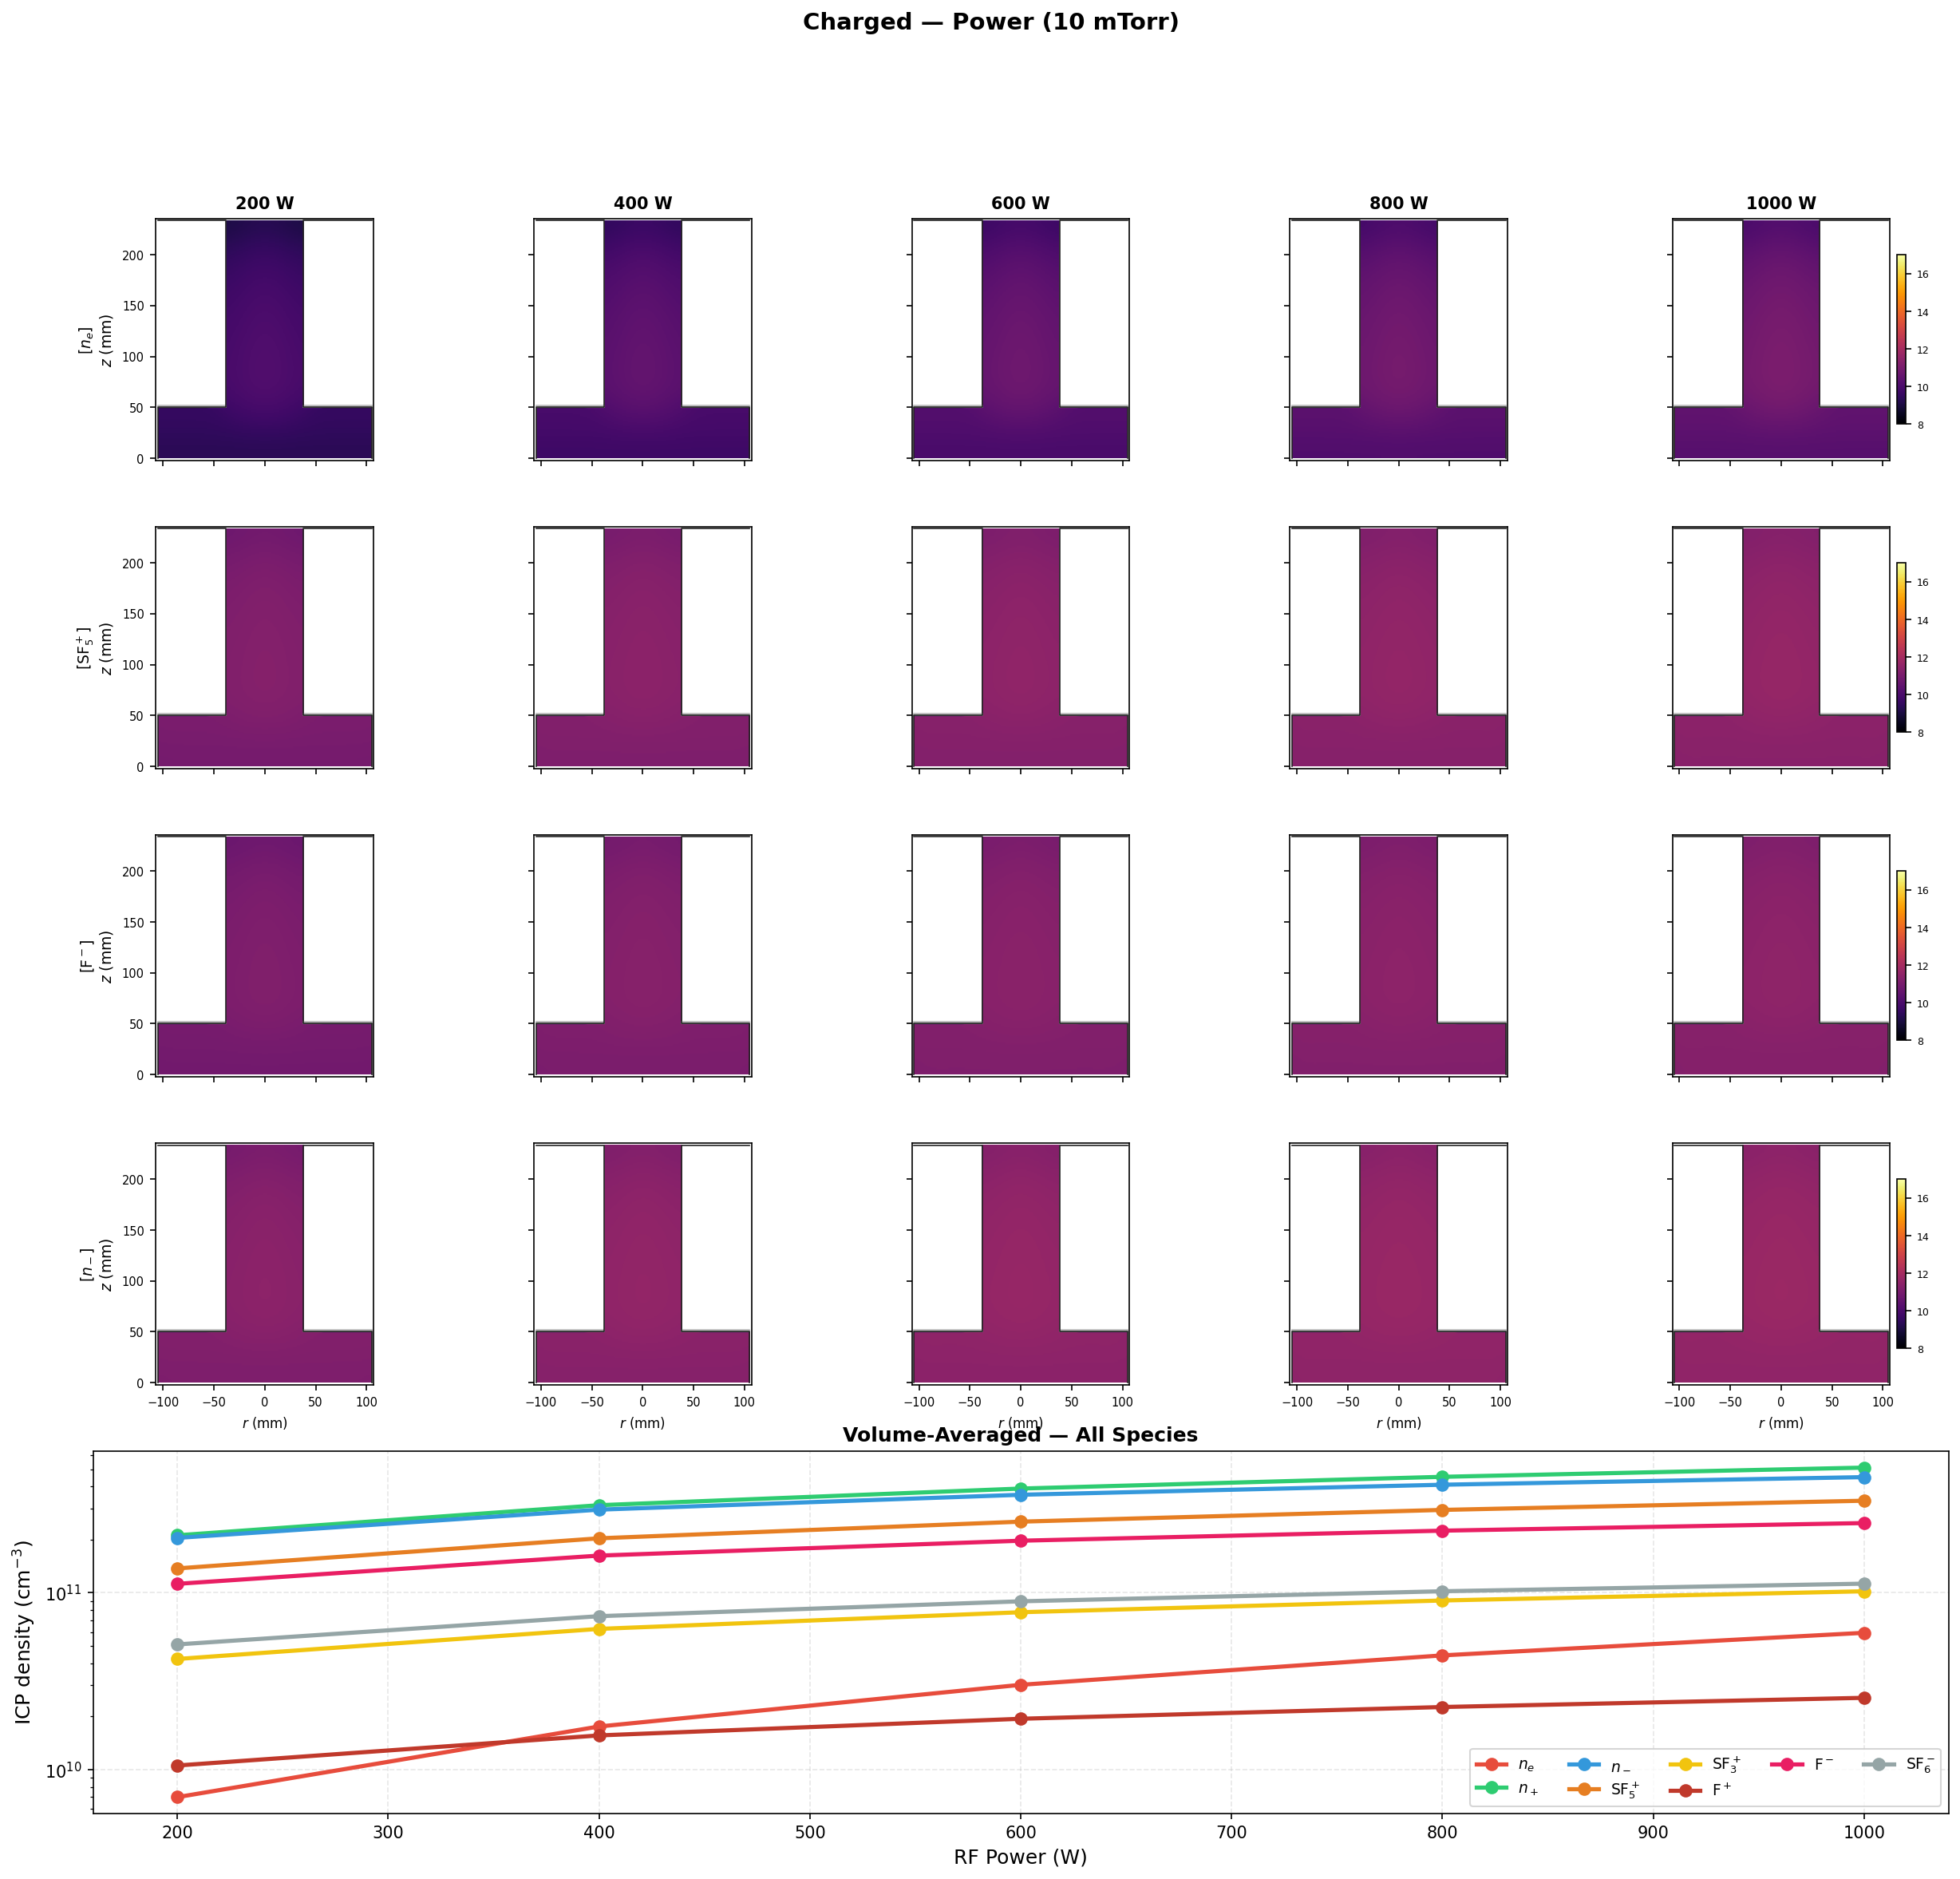
\includegraphics[width=\textwidth]{charged_power_2D.png}
    \caption{Charged species vs.\ RF power.}
    \label{fig:charged_power}
  \end{subfigure}
  \hfill
  \begin{subfigure}[t]{0.48\textwidth}
    \centering
    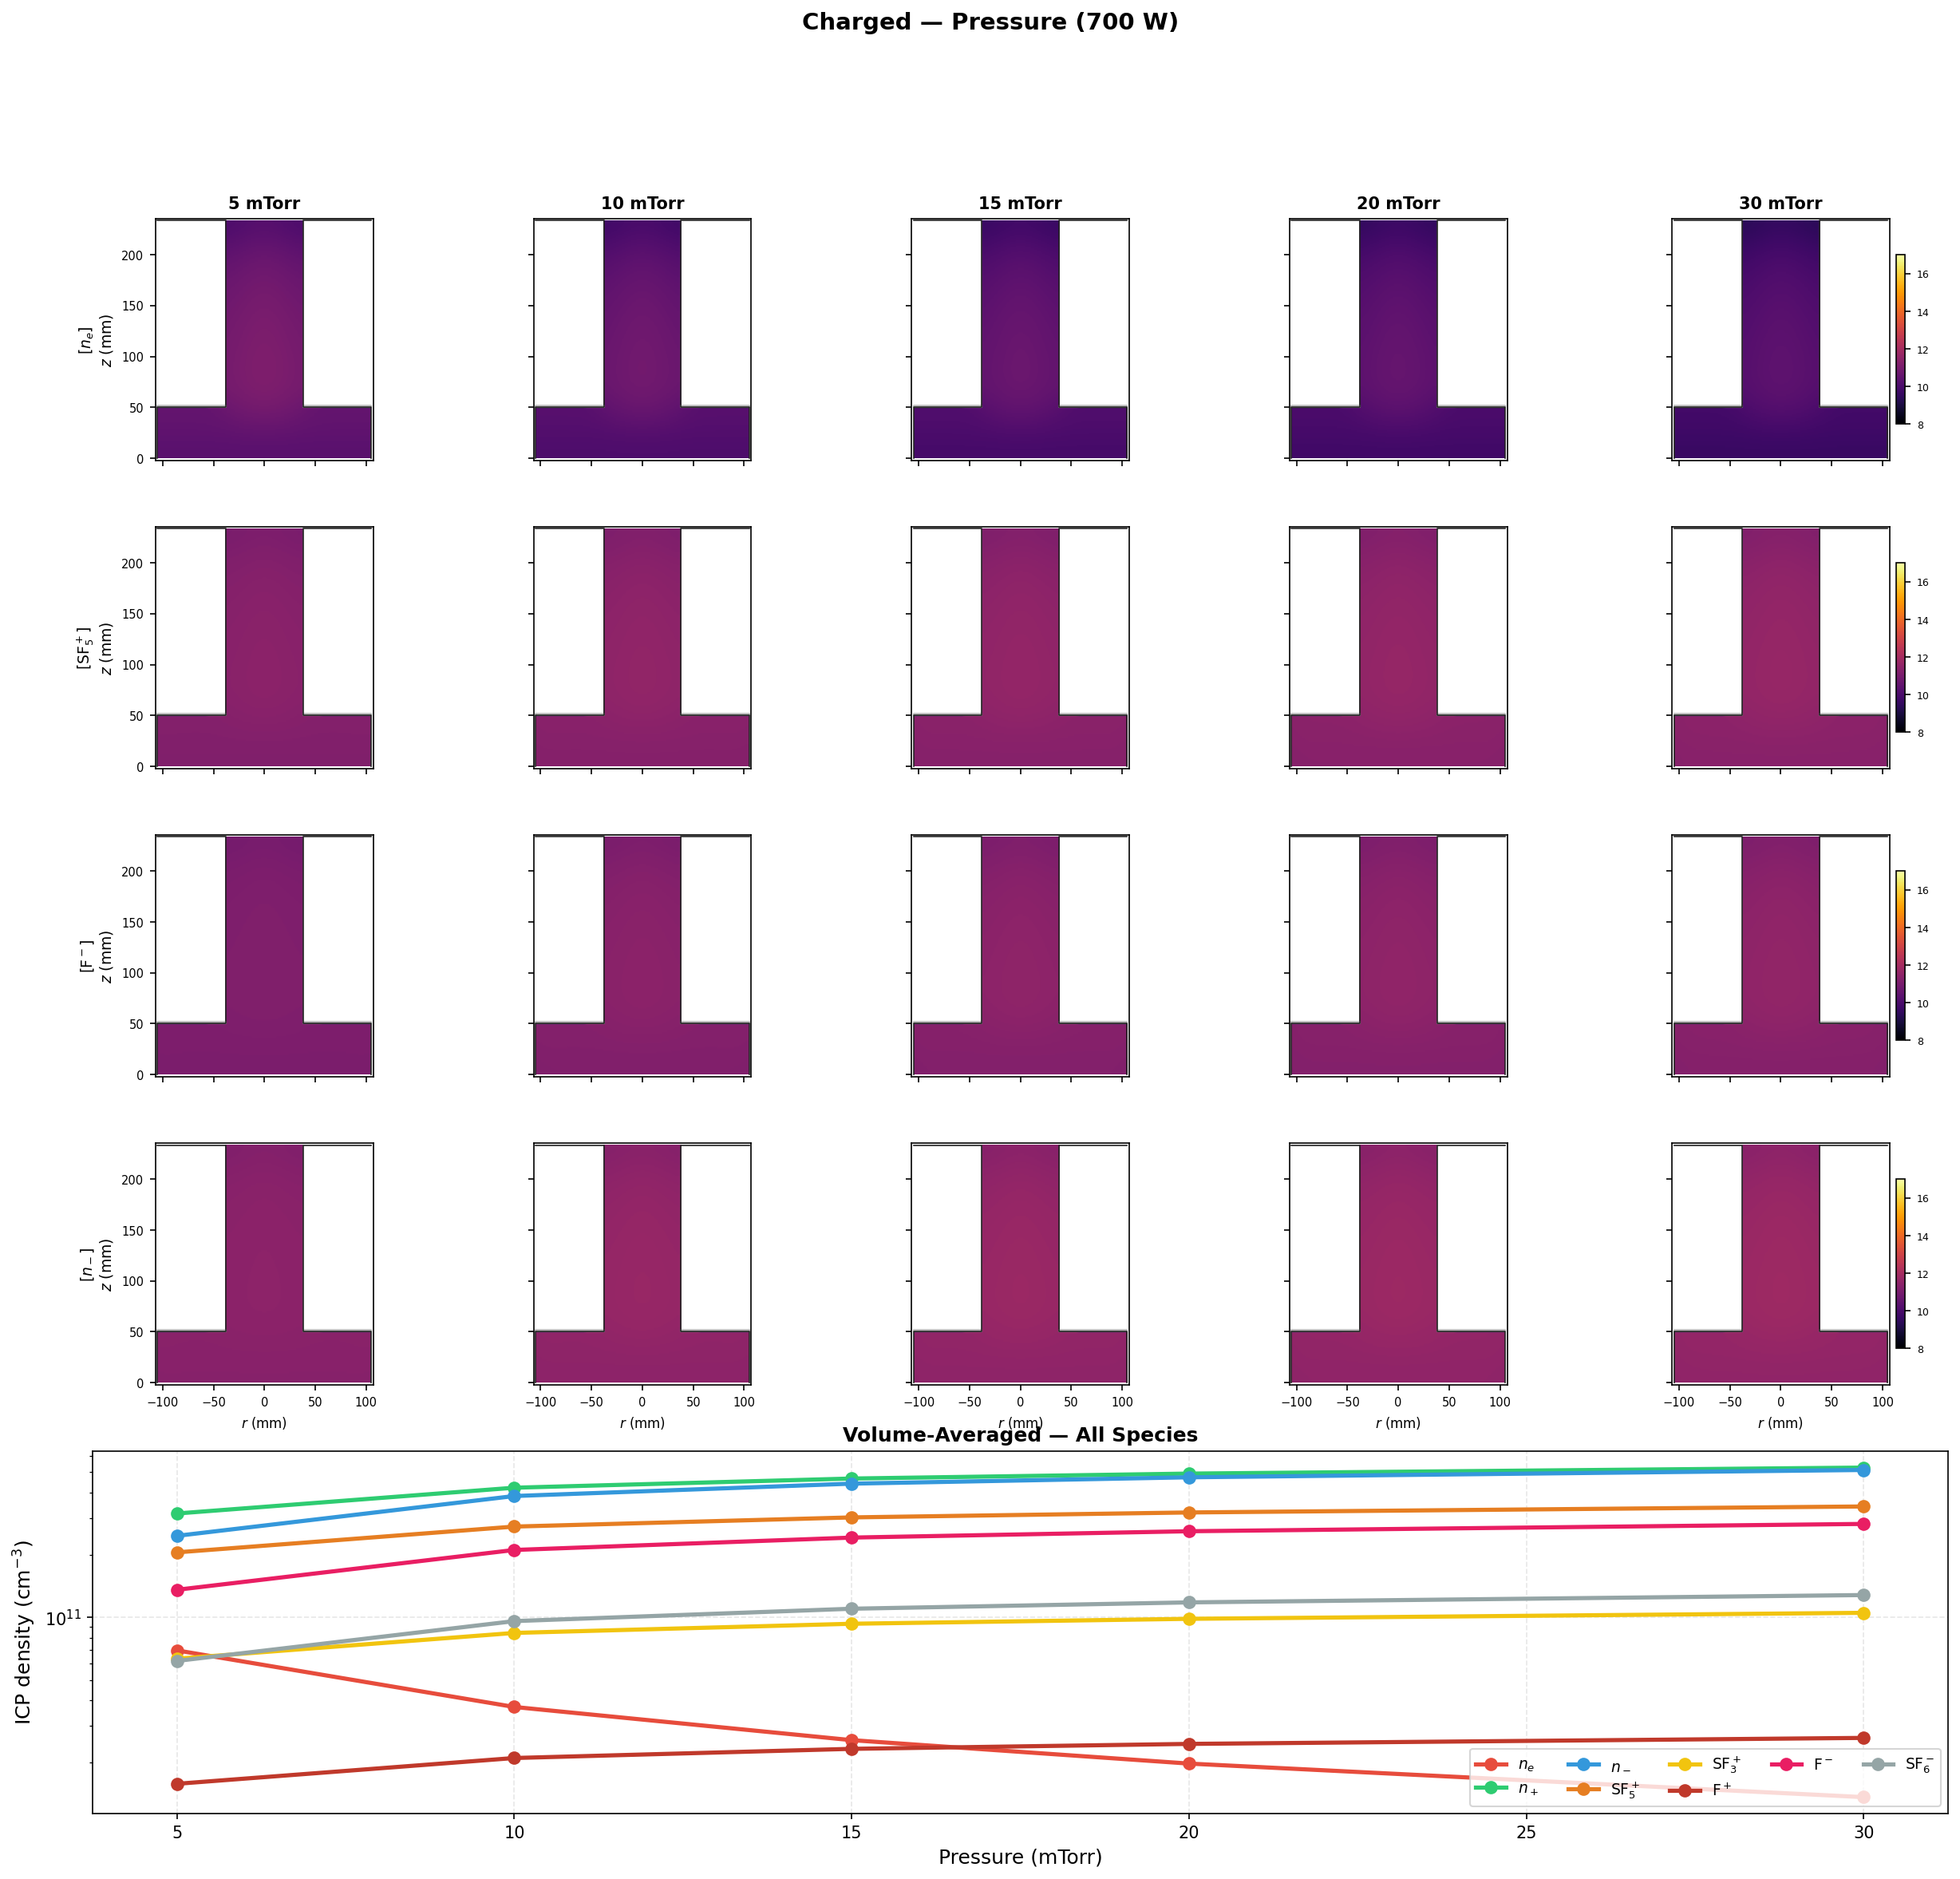
\includegraphics[width=\textwidth]{charged_pressure_2D.png}
    \caption{Charged species vs.\ pressure.}
    \label{fig:charged_pressure}
  \end{subfigure}
  \caption{Parameter sweeps showing the dependence of neutral and
           charged species on RF power and gas pressure.}
  \label{fig:sweeps}
\end{figure}

\begin{figure}[H]
  \centering
  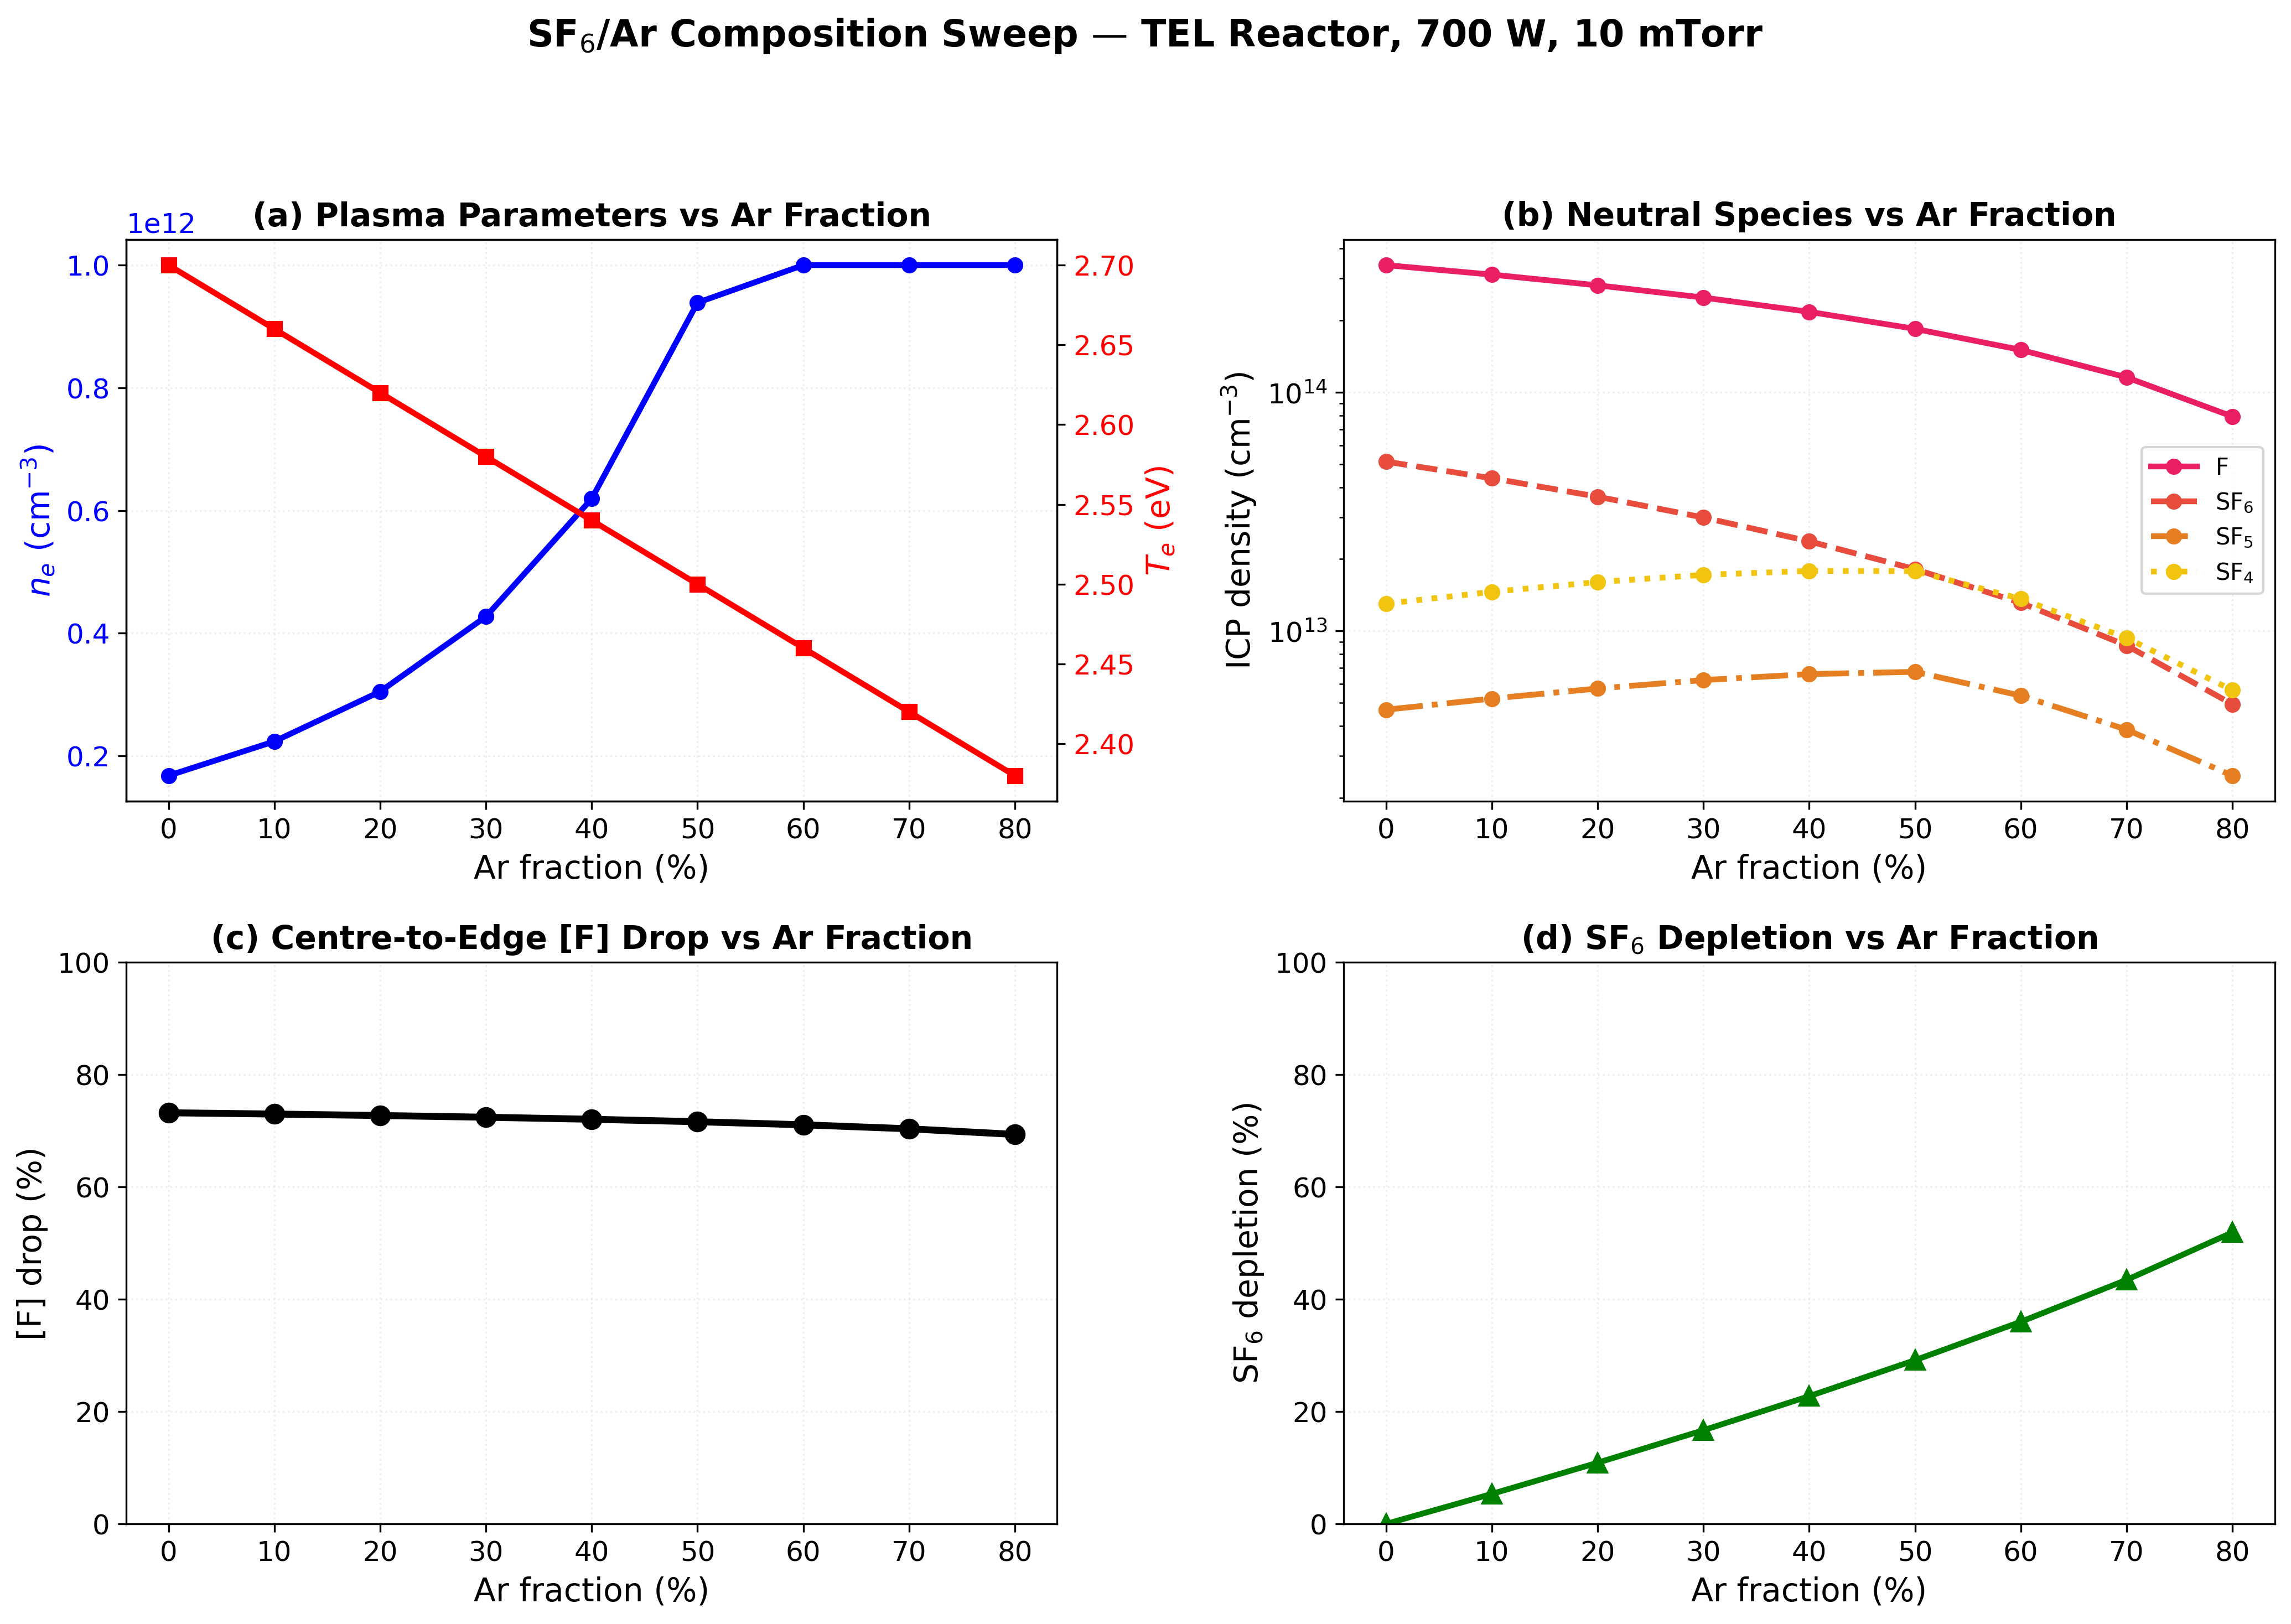
\includegraphics[width=0.65\textwidth]{composition_sweep.png}
  \caption{Effect of Ar fraction on species densities.  Increasing Ar
           dilution reduces SF\textsubscript{6} dissociation products
           while raising the electron density due to the lower
           ionisation threshold of Ar.}
  \label{fig:composition}
\end{figure}

\begin{figure}[H]
  \centering
  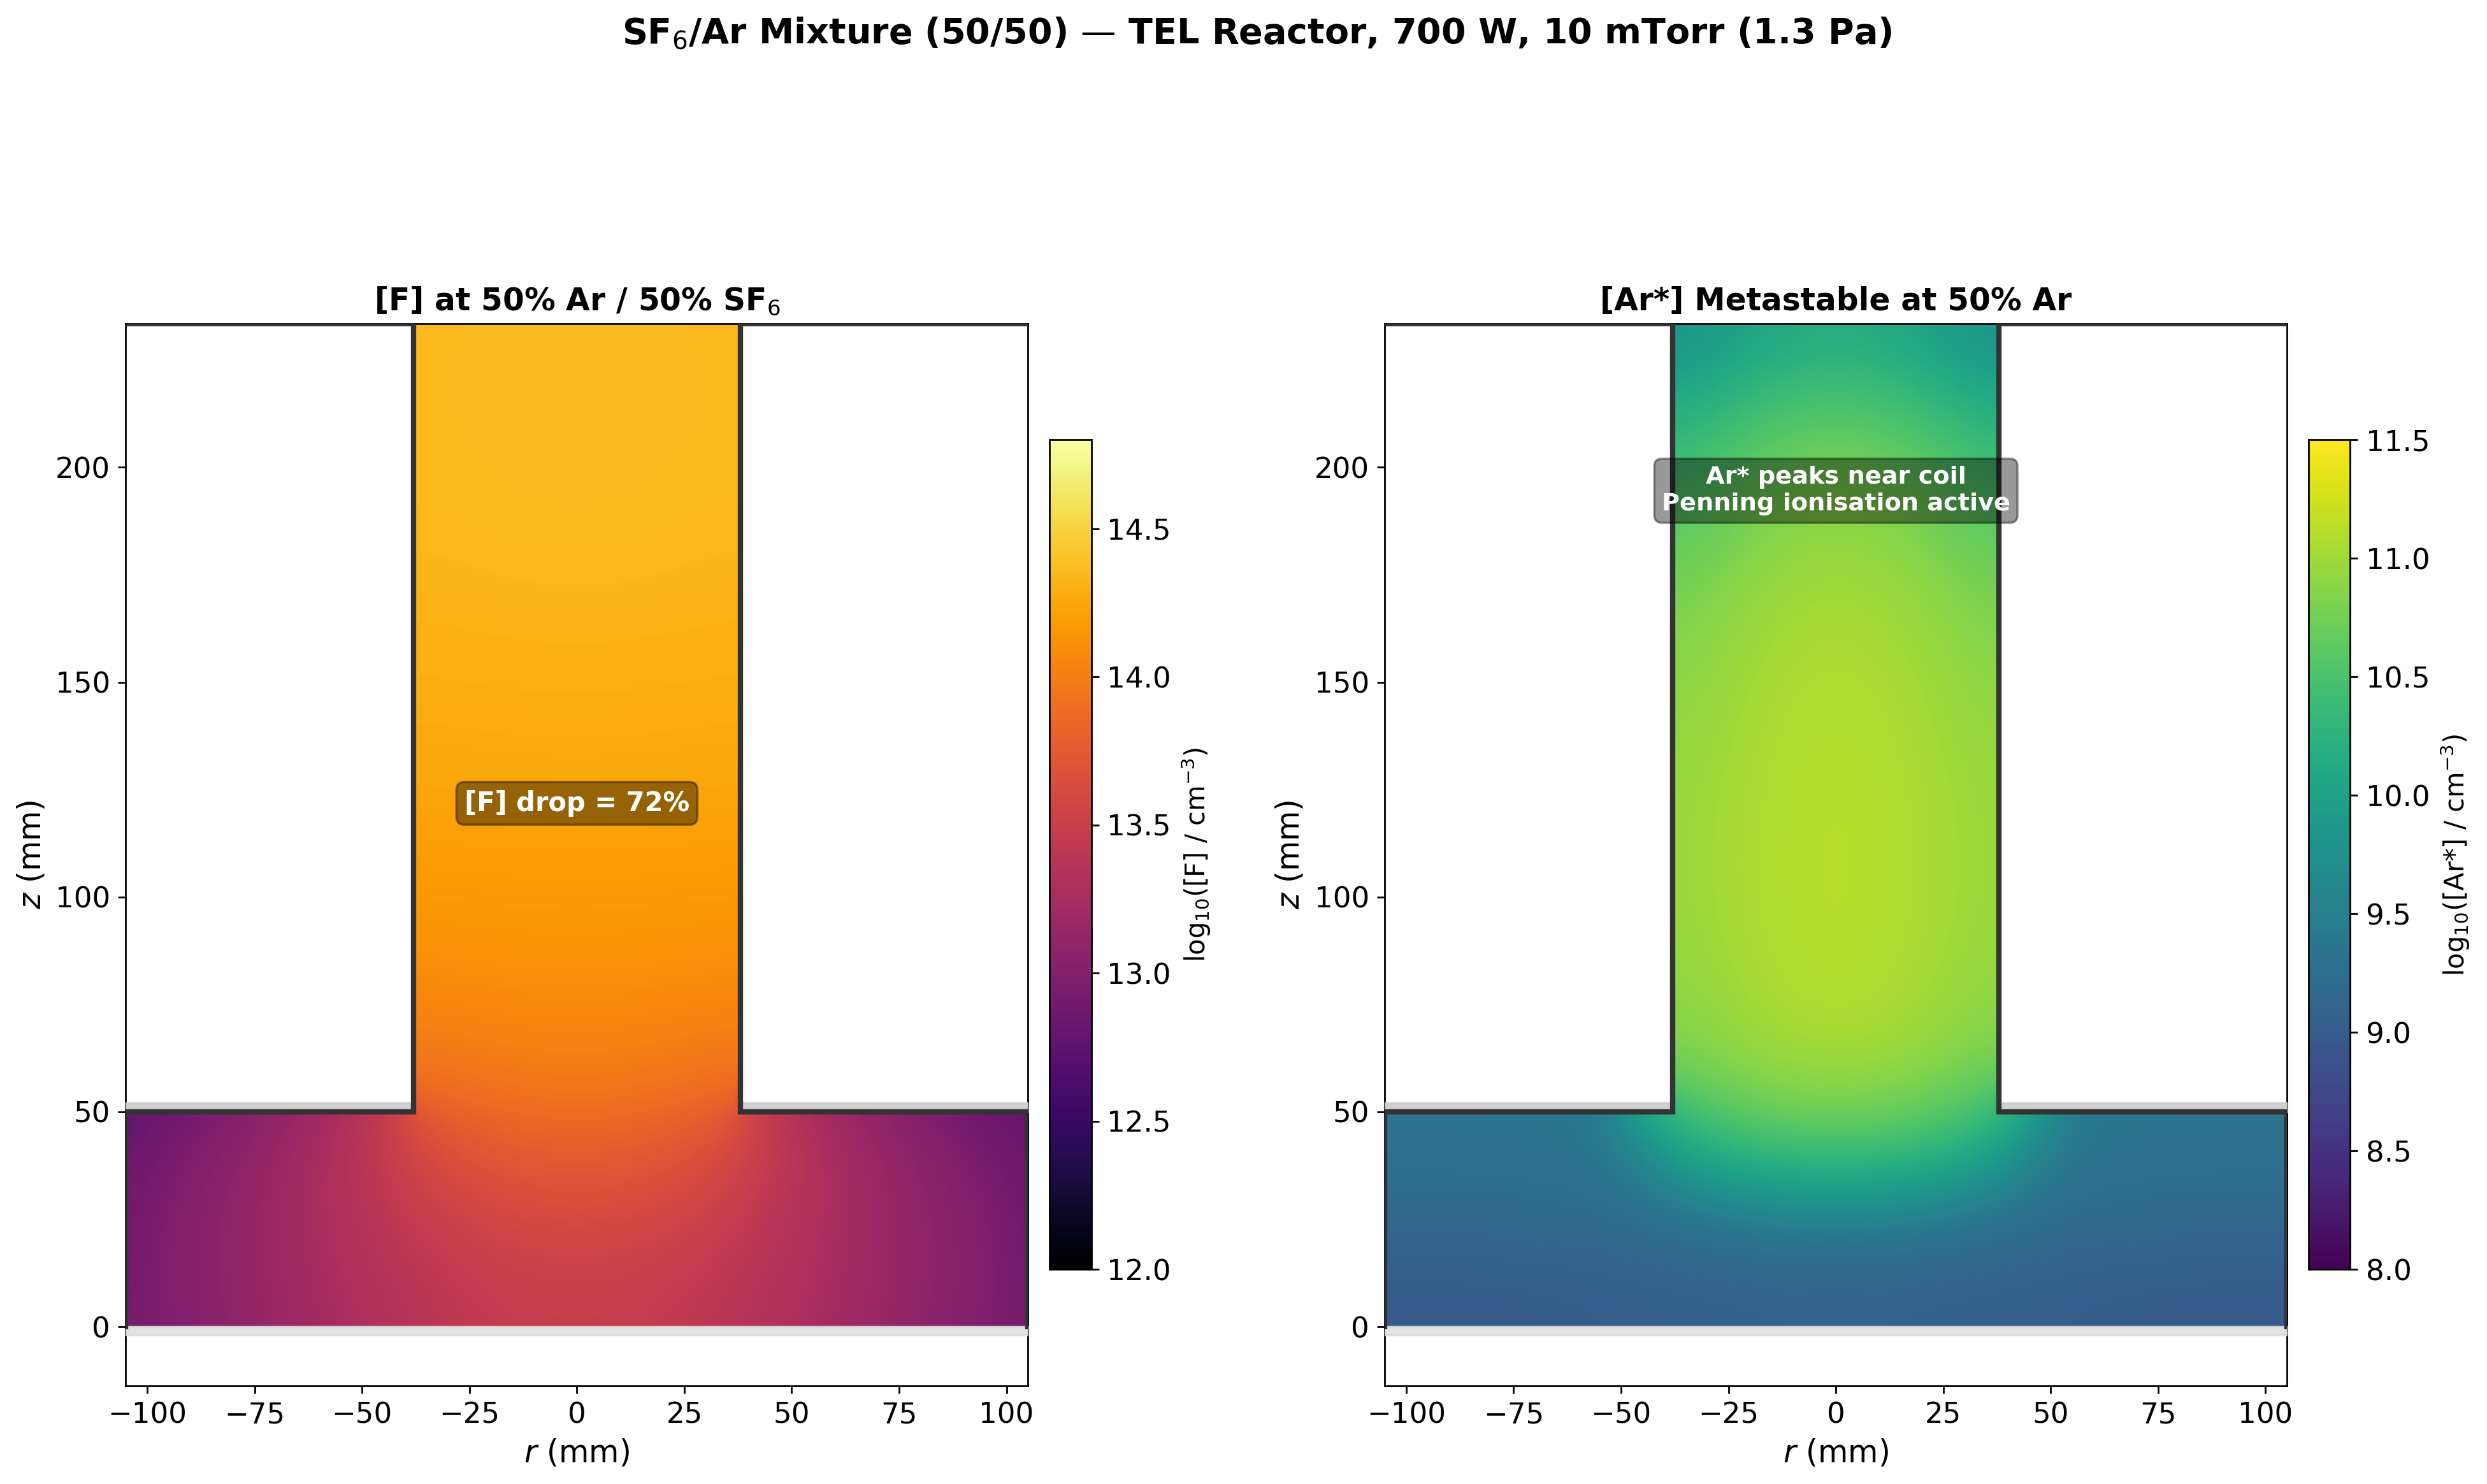
\includegraphics[width=0.65\textwidth]{Ar_contours.png}
  \caption{Spatial distribution of Ar metastable and Ar$^+$ densities
           at 30\% Ar fraction, showing the characteristic
           skin-depth confinement.}
  \label{fig:ar_contours}
\end{figure}

\begin{figure}[H]
  \centering
  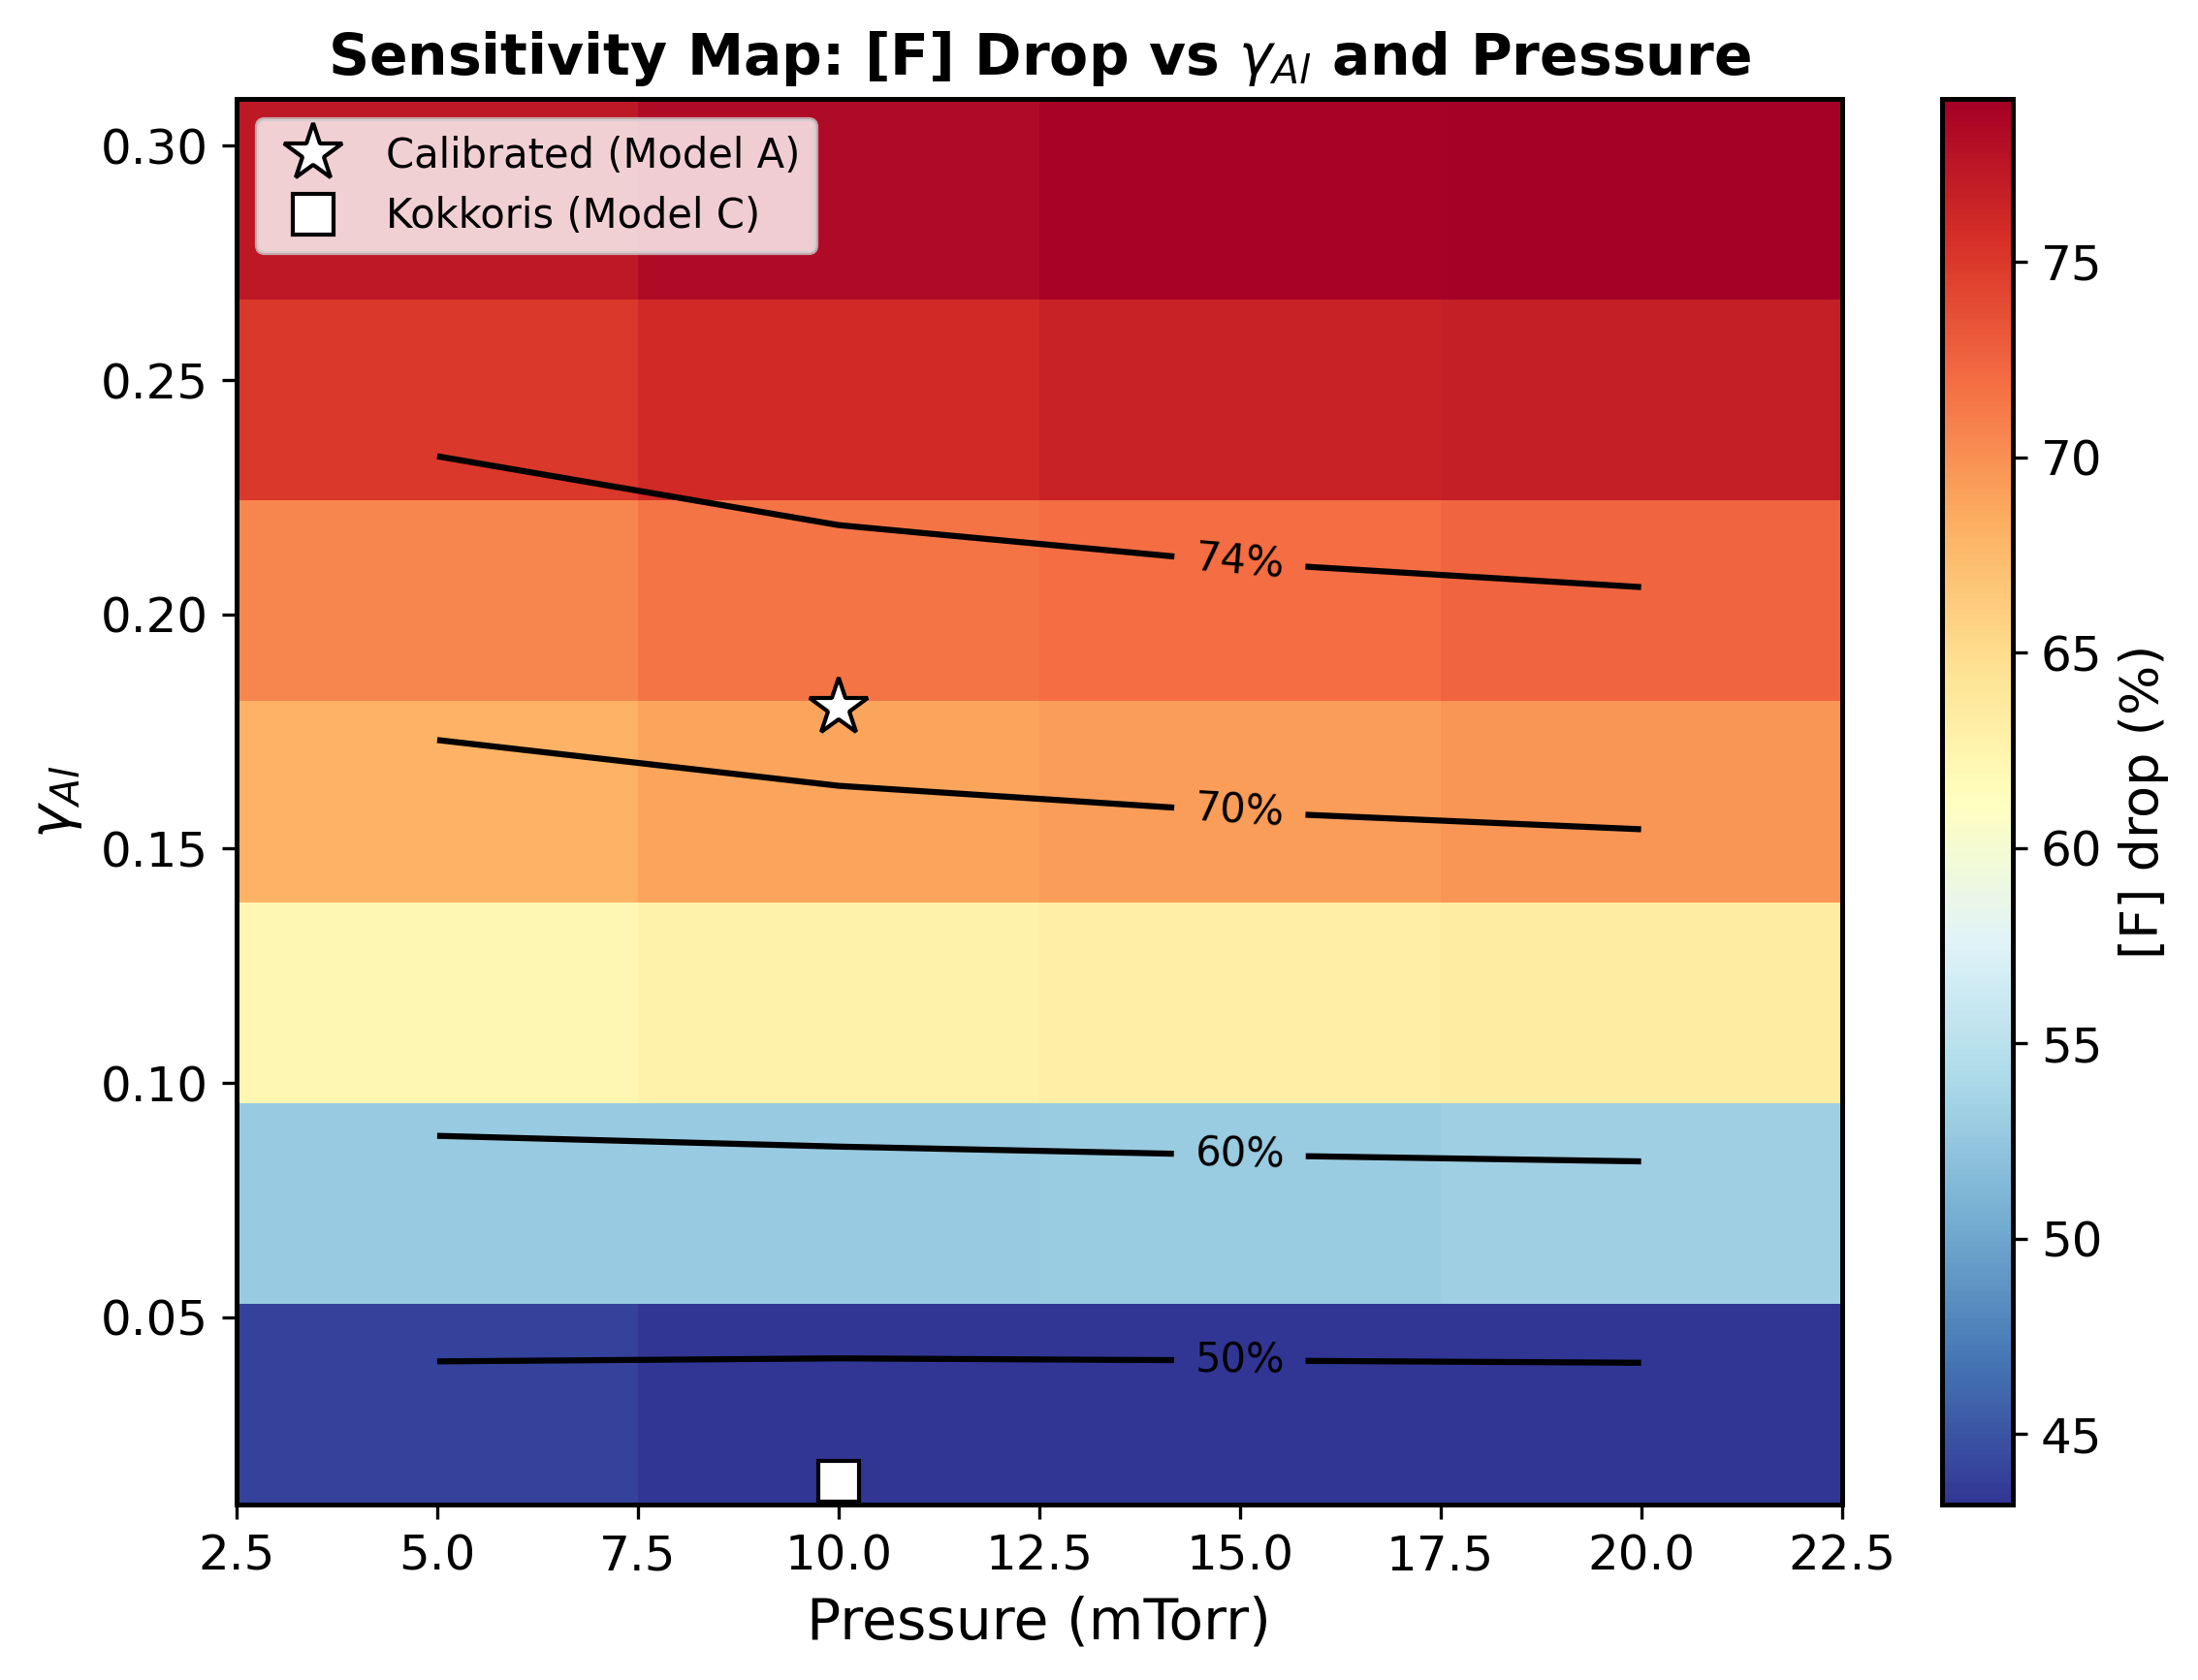
\includegraphics[width=0.65\textwidth]{sensitivity_map.png}
  \caption{Sensitivity map showing the partial derivatives
           $\partial \ln n_{\text{F}} / \partial x_i$ for each input
           parameter.  RF power and pressure dominate; Ar fraction
           has a secondary but non-negligible effect.}
  \label{fig:sensitivity}
\end{figure}

Figure~\ref{fig:wafer_diag} shows wafer-level diagnostics: the
radial F profile that governs etch uniformity and the species flux
budget at the wafer surface.

\begin{figure}[H]
  \centering
  \begin{subfigure}[t]{0.48\textwidth}
    \centering
    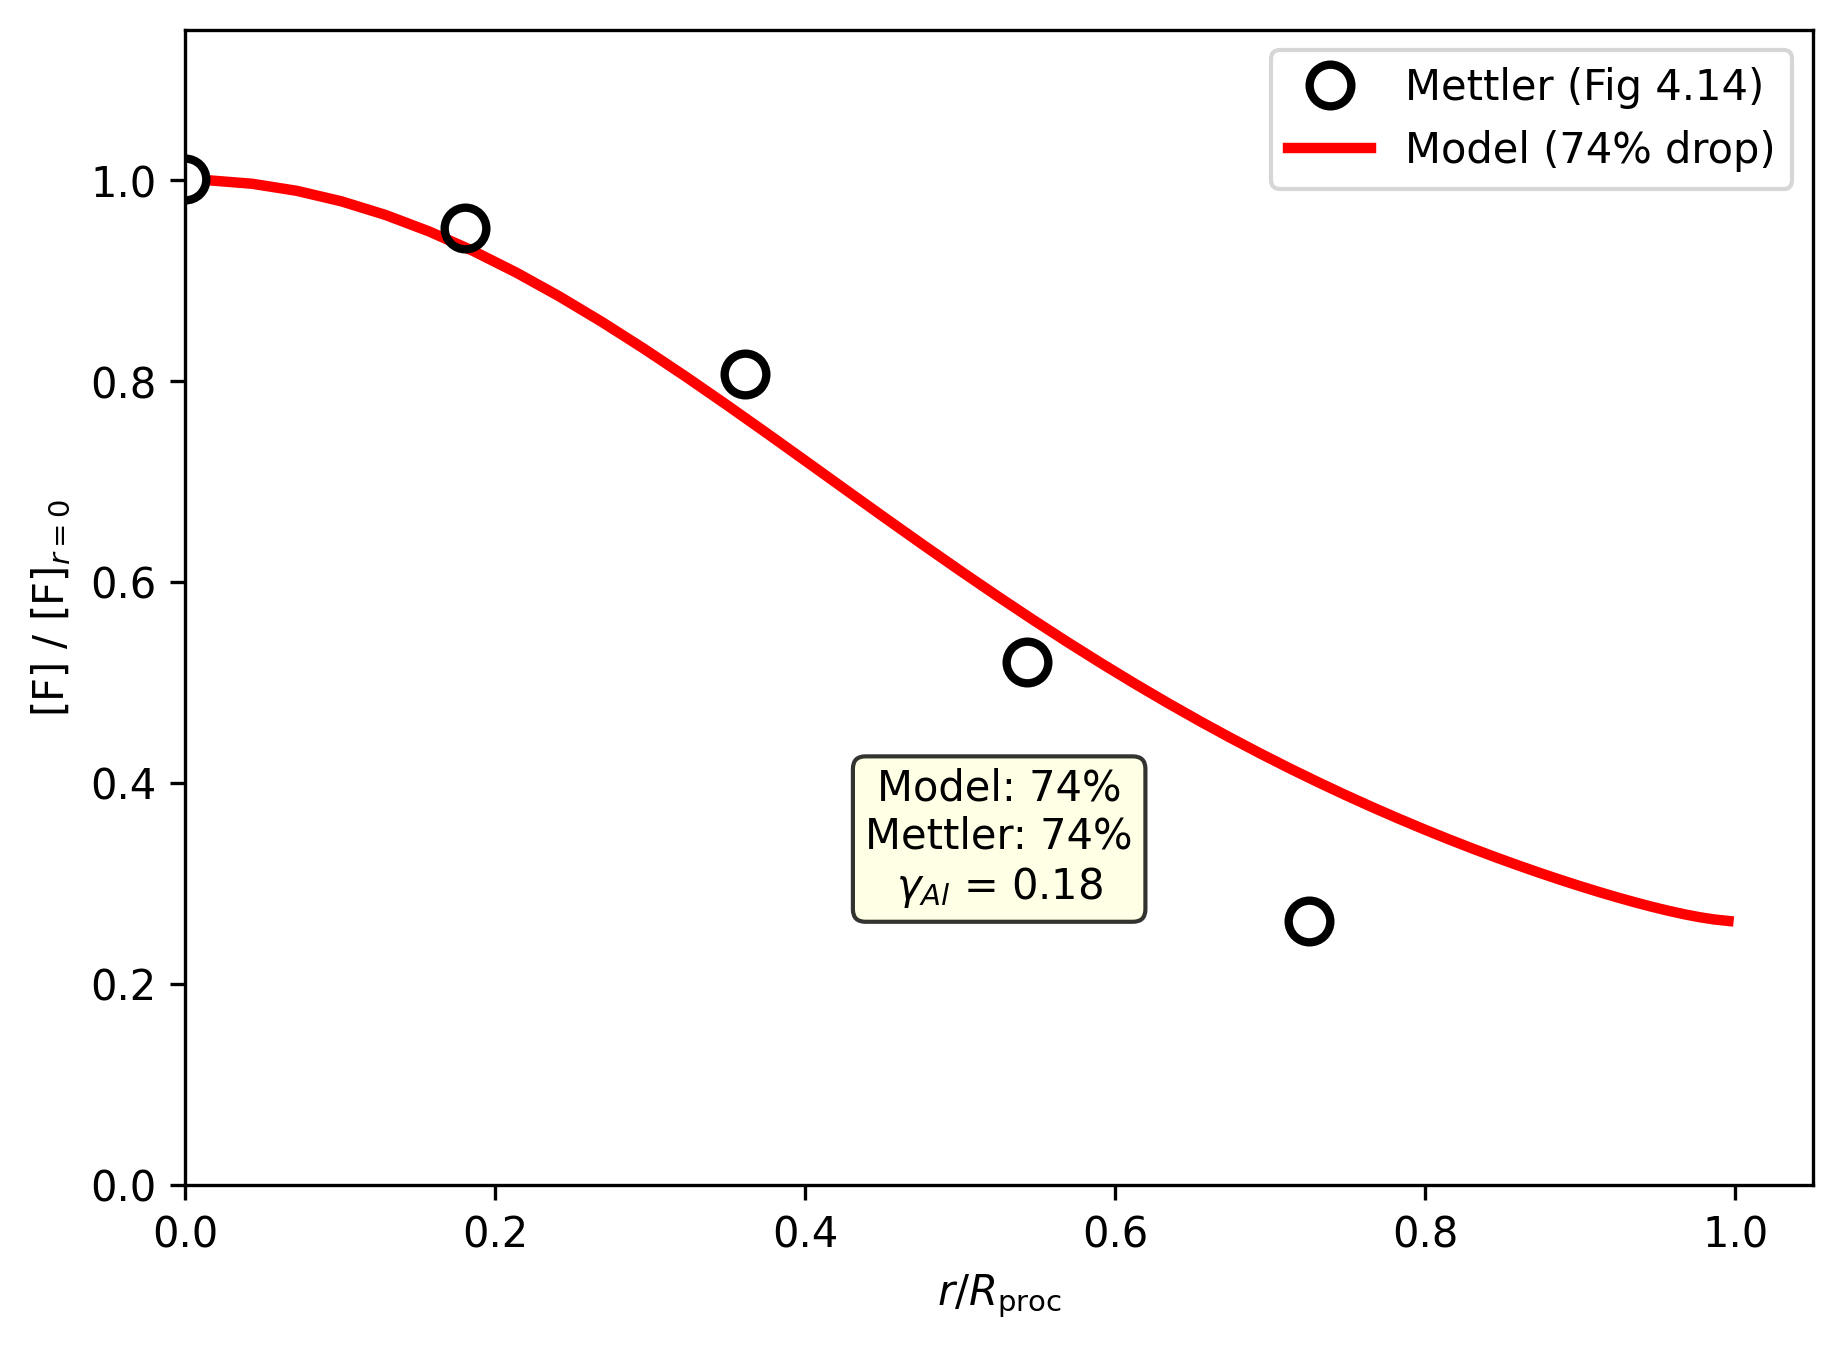
\includegraphics[width=\textwidth]{radial_F_profile.png}
    \caption{Radial F density profile at the wafer.}
    \label{fig:radial_F}
  \end{subfigure}
  \hfill
  \begin{subfigure}[t]{0.48\textwidth}
    \centering
    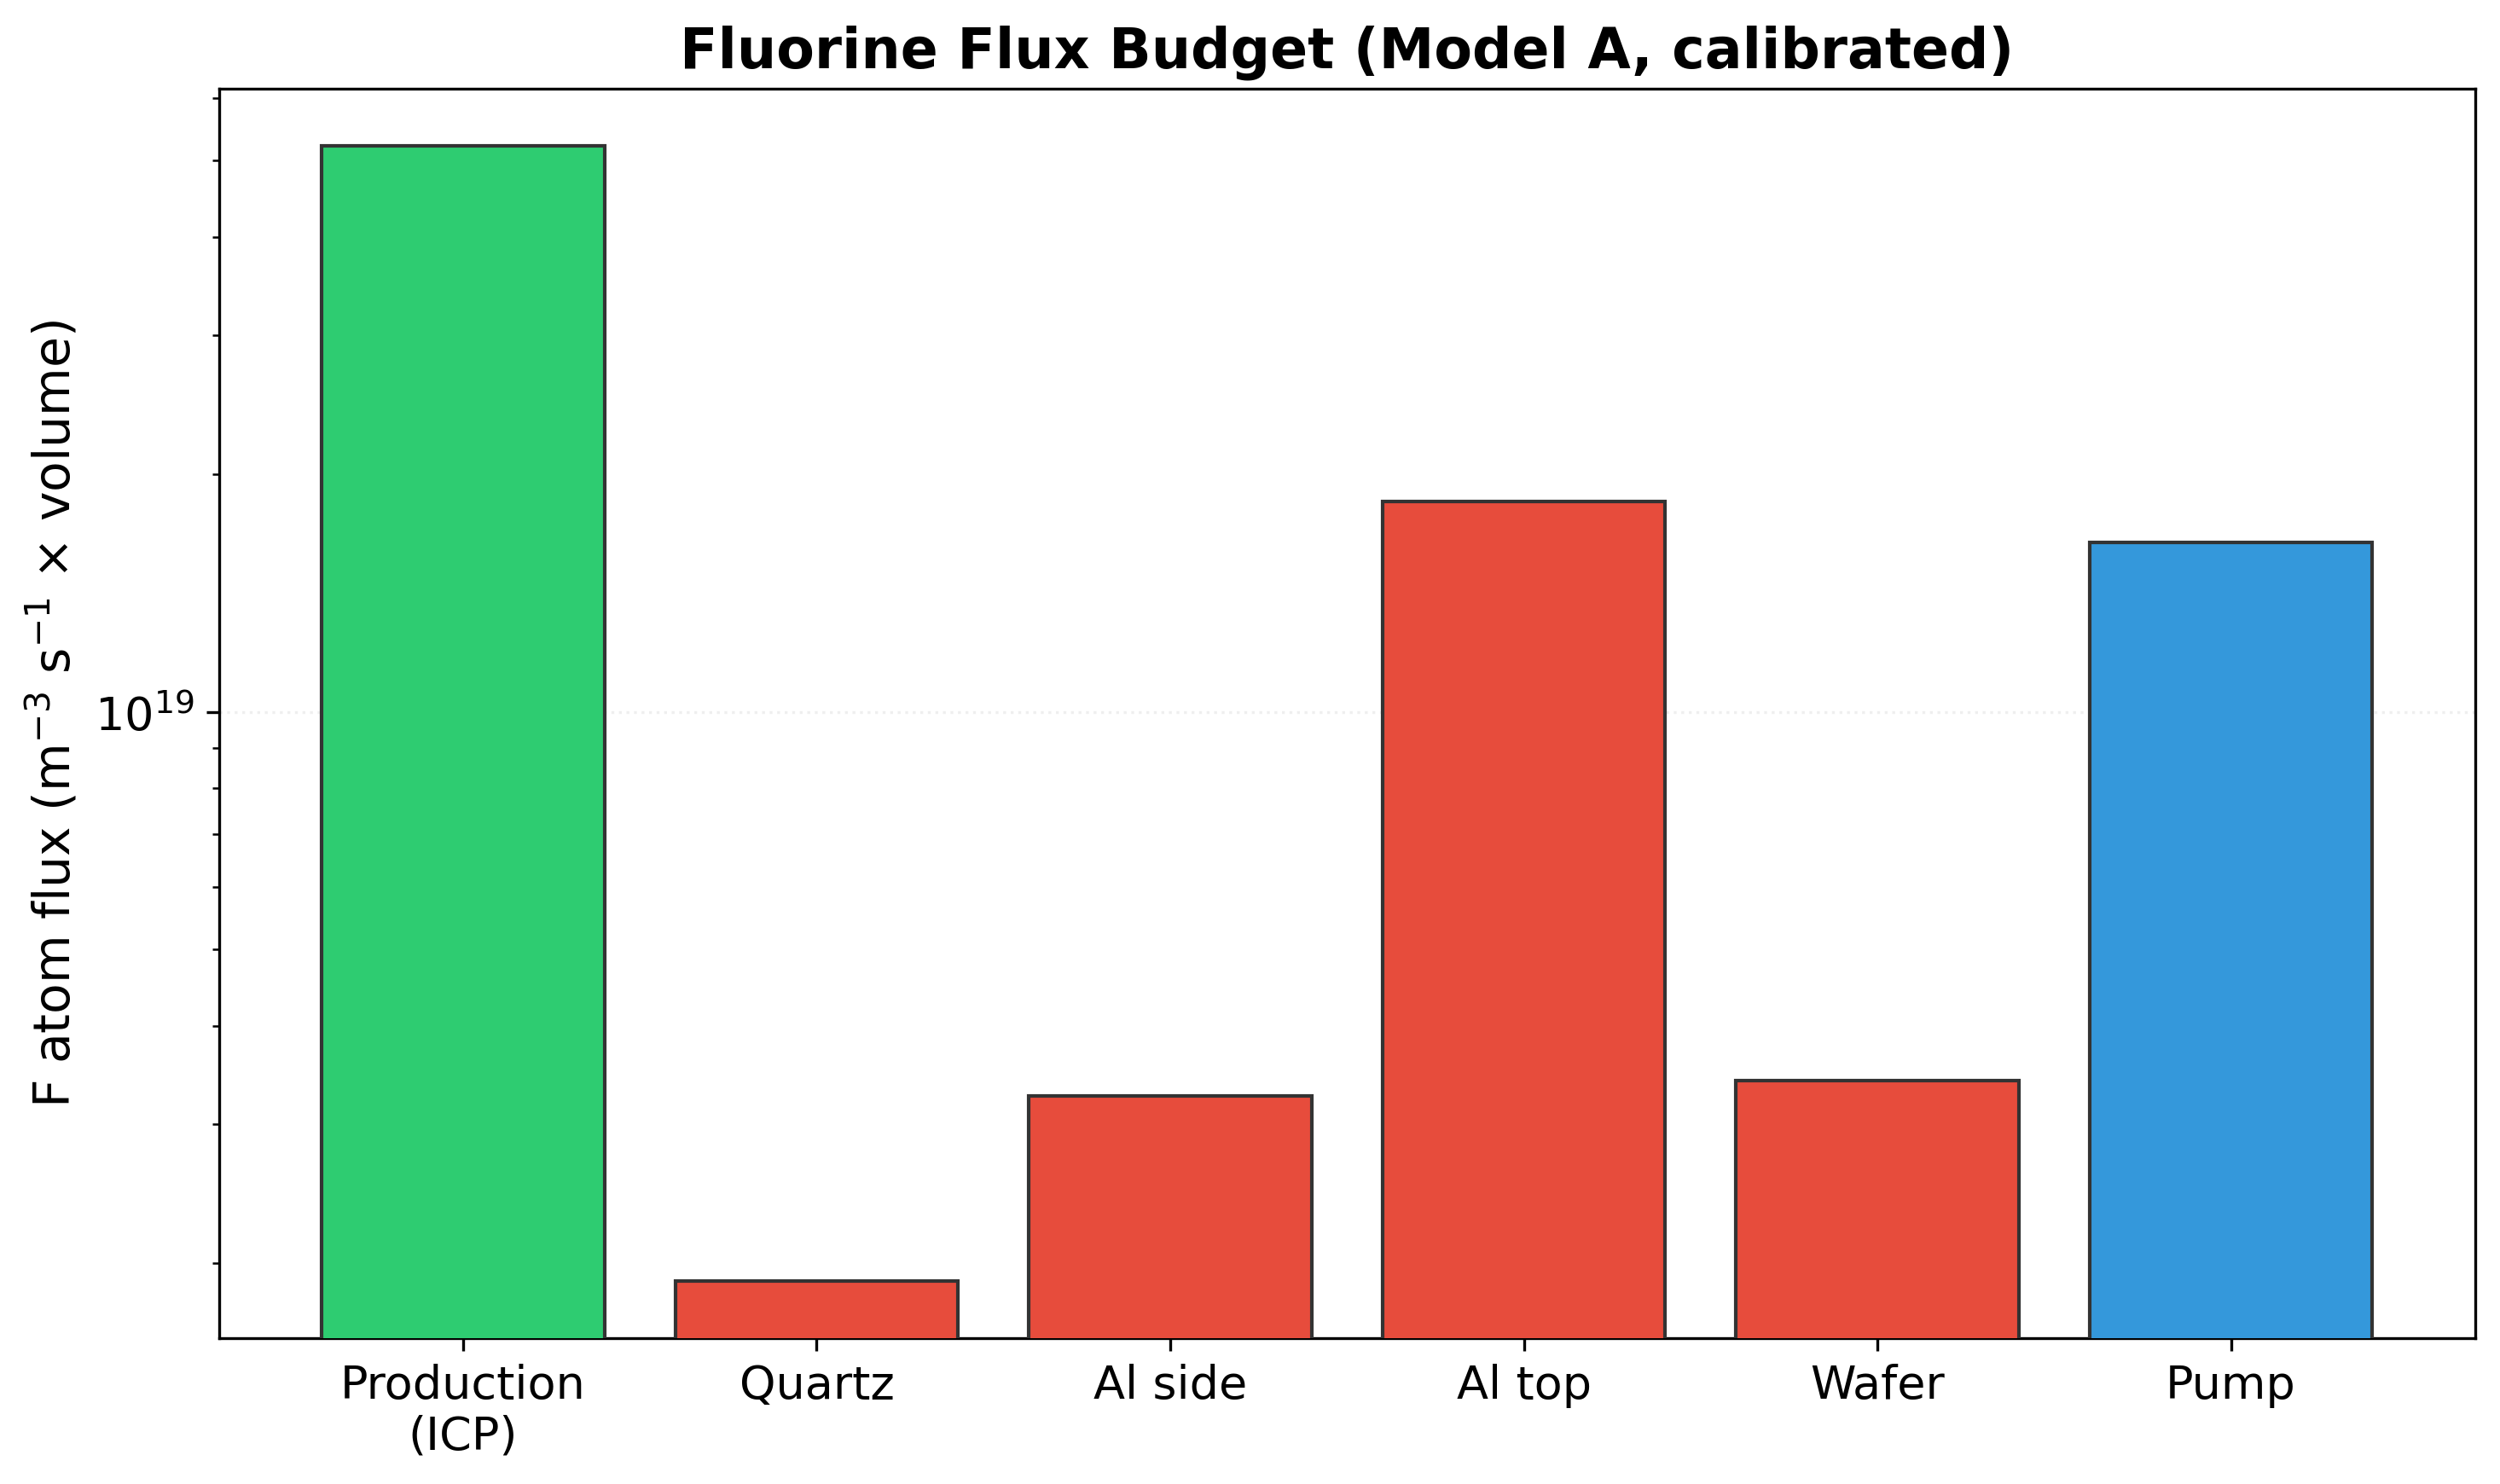
\includegraphics[width=\textwidth]{flux_budget.png}
    \caption{Species flux budget at the wafer surface.}
    \label{fig:flux}
  \end{subfigure}
  \caption{Wafer-level diagnostics.  The radial F profile governs etch
           uniformity; the flux budget shows the balance between
           diffusive supply and wall recombination.}
  \label{fig:wafer_diag}
\end{figure}

\begin{figure}[H]
  \centering
  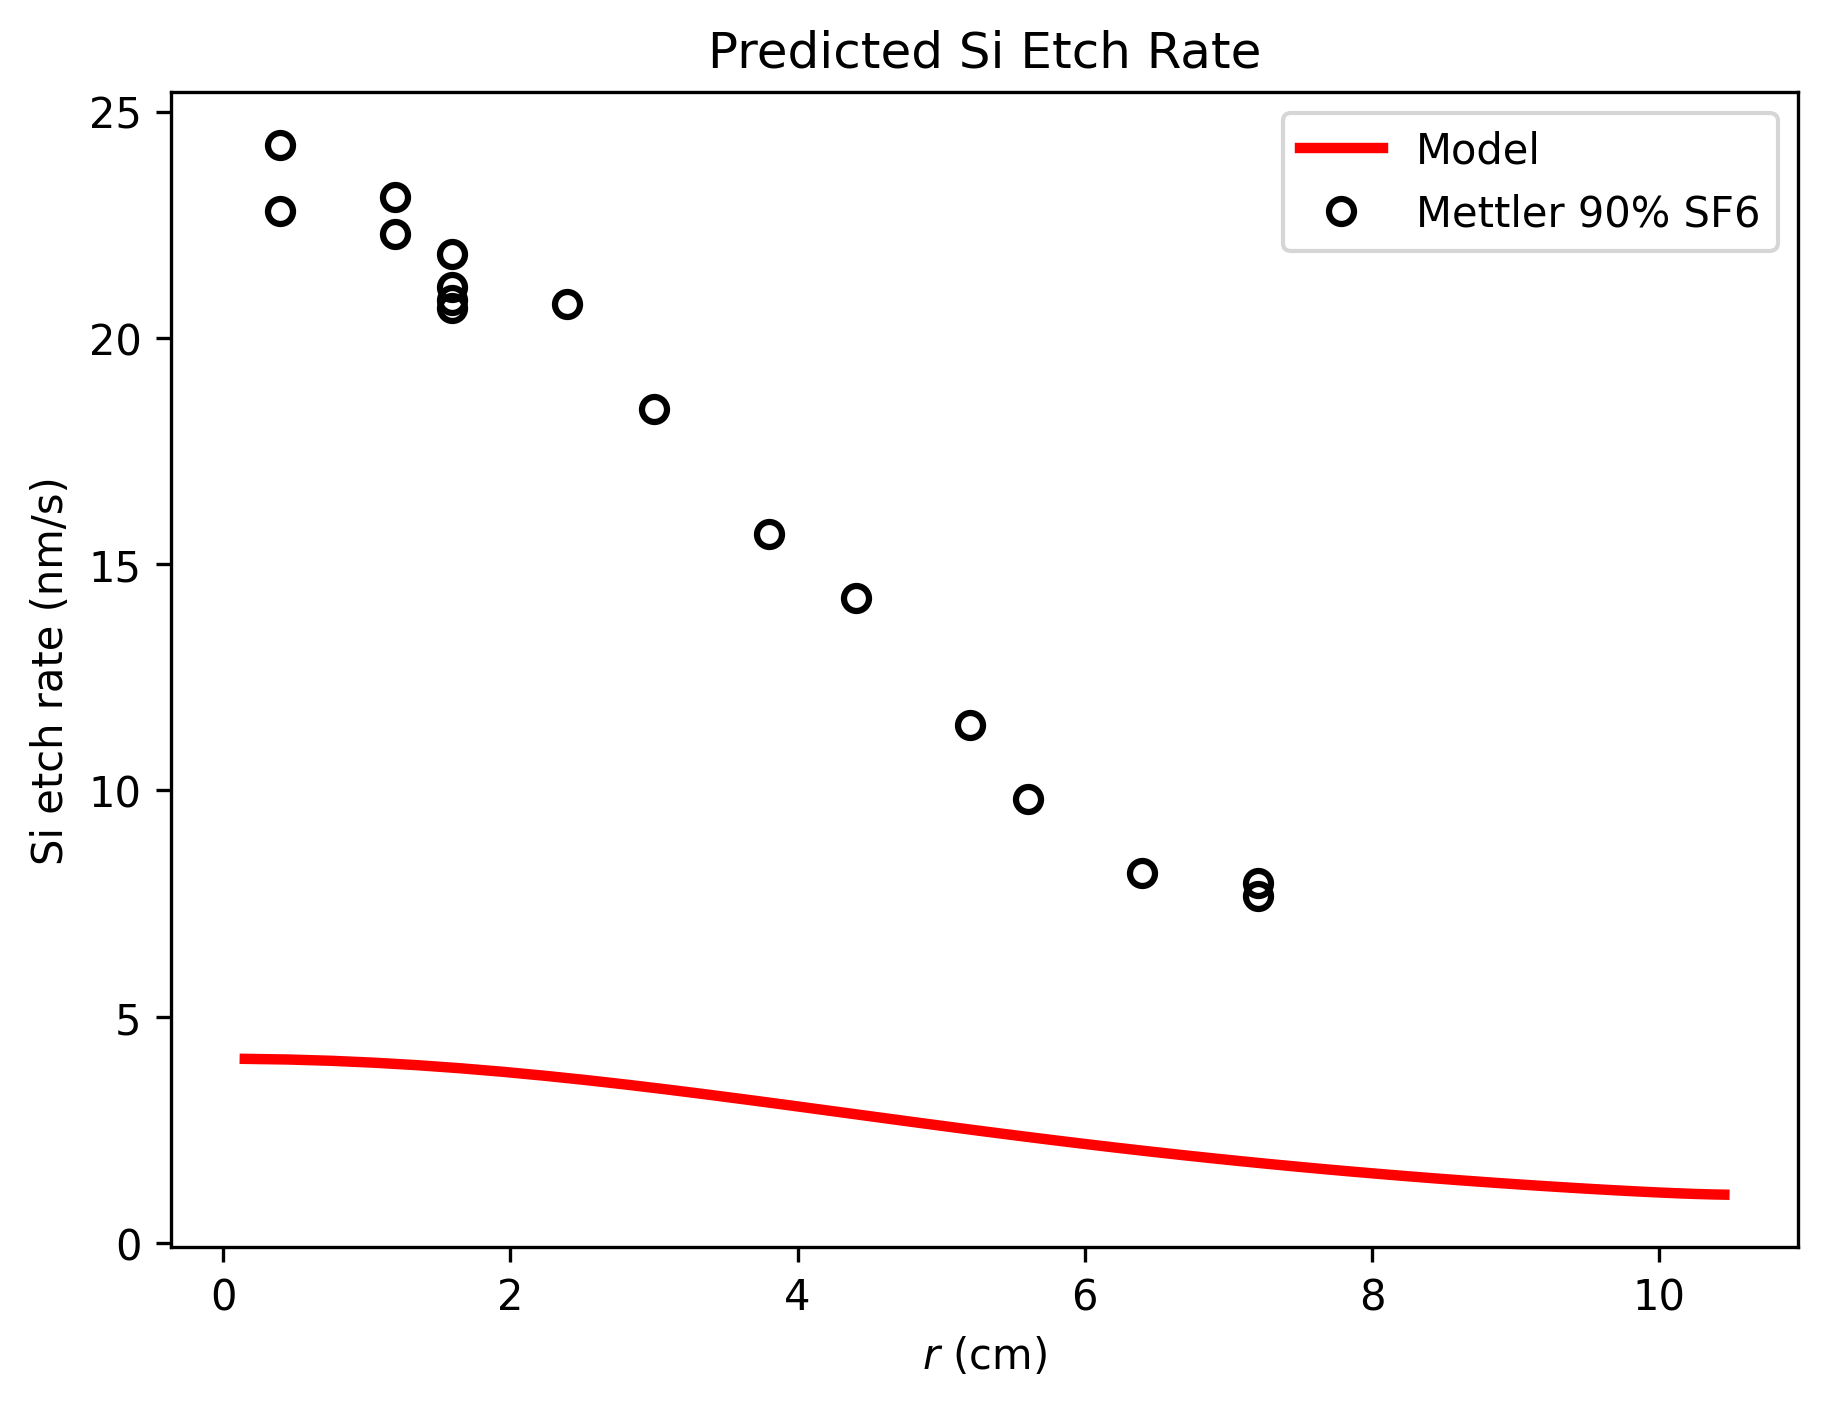
\includegraphics[width=0.55\textwidth]{etch_rate.png}
  \caption{Predicted etch rate as a function of radial position on the
           wafer, computed from the F flux and the Arrhenius surface
           reaction model.  The centre-to-edge variation quantifies
           the etch non-uniformity.}
  \label{fig:etch_rate}
\end{figure}

% ==================================================================
\section{Supplementary Experiments}
\label{sec:supplementary}

Three supplementary experiments were conducted to test alternative
training strategies.  All three produced negative results, confirming
the robustness of the chosen approach.

\subsection{Transfer Learning}

Pre-training on the legacy dataset and fine-tuning on LXCat data
yields nF RMSE = 0.00375, compared to 0.00385 for training from
scratch.  The negligible improvement confirms that the two datasets
have effectively identical statistical structure (consistent with the
dataset diagnosis in Section~\ref{sec:dataset_diagnosis}).  Transfer
learning offers \textbf{no benefit} for this problem.

\subsection{$T_e$ Auxiliary Head}

Adding an auxiliary head to predict electron temperature degrades the
primary nF RMSE from 0.0038 to 0.00424.  The $T_e$ field has
fundamentally different spatial structure (concentrated in the ICP
source) and competes for representational capacity in the shared
trunk.  Adding $T_e$ prediction \textbf{hurts nF} performance.

\subsection{Mixed-Physics Training}

Training a single surrogate on both legacy and LXCat data
simultaneously hurts both targets: nF RMSE = 0.0057 (legacy) and
0.0229 (LXCat).  The cross-section differences produce incompatible
density fields at the same operating conditions, creating conflicting
training signals.  Mixed-physics training \textbf{hurts both}
datasets.

% ==================================================================
\section{Computational Cost and Experiment Timeline}
\label{sec:compute}

The full experimental campaign consumed \textbf{97.4~GPU/CPU-hours}
across 13 experiment categories.
Table~\ref{tab:compute} provides a detailed breakdown.

\begin{table}[H]
  \centering
  \caption{Computational cost by experiment category.  Total:
           97.4~hours across 13 categories.}
  \label{tab:compute}
  \small
  \begin{tabular}{@{}llcl@{}}
    \toprule
    Experiment & Runs & Compute (hrs) & Key metric \\
    \midrule
    Dataset generation (LXCat~v3) & 221 cases & 0.2
      & 0 failures \\
    Architecture sweep (E0--E6) & 21 & 11.4
      & E3 wins: nF\,=\,0.00210 \\
    Ablation study & 15 & 21.8
      & bias\_only: nF\,=\,0.00314 \\
    Production ensemble & 5 & 7.9
      & nF\,=\,0.00154 \\
    Transfer learning & 6 & 17.7
      & No benefit \\
    Mixed-physics training & 3 & 19.4
      & Hurts both regimes \\
    $T_e$ auxiliary head & 3 & 16.5
      & Hurts nF by 11\% \\
    ML baselines (GP + poly) & 3 & 2.2
      & GP\,=\,0.006, poly\,=\,0.039 \\
    Mesh convergence & 6 & $<$0.1
      & 1.86\% nF error \\
    Speedup measurement & 40 & $<$0.1
      & 531$\times$ / 874$\times$ \\
    Spatial error analysis & --- & $<$0.1
      & Uniform across regions \\
    Literature validation & 10 & $<$0.1
      & F 36\%, $T_e$ 5\%/58\% \\
    Dataset diagnosis & --- & $<$0.1
      & Datasets identical \\
    \bottomrule
  \end{tabular}
\end{table}

The compute budget divides naturally into three tiers.
\textbf{Core experiments}---the architecture sweep (11.4~h),
ablation study (21.8~h), and production ensemble (7.9~h)---account
for 41.1~hours and produced all positive results reported in this
paper.  \textbf{Supplementary experiments}---transfer learning
(17.7~h), mixed-physics training (19.4~h), and the $T_e$ auxiliary
head (16.5~h)---consumed 53.6~hours, more than the core experiments,
yet all three yielded negative results.  The remaining 2.7~hours
cover fast validation tasks (ML baselines, mesh convergence, speedup
measurement, spatial error analysis, literature validation, and
dataset diagnosis) that required negligible compute.

That the supplementary experiments dominate the compute budget is
noteworthy.  The ablation study alone required 21.8~hours because
five configurations were each trained with three seeds, and training
to convergence on the LXCat dataset is inherently expensive.
Transfer learning (17.7~h) and mixed-physics training (19.4~h) each
required multiple full training runs with different pre-training and
data-mixing strategies.  While none of these experiments improved
the production surrogate, they preemptively answer likely reviewer
questions: ``Did you try transfer learning?'' (yes---no benefit),
``Can a single model handle both cross-section sets?'' (no---it
hurts both), and ``Does predicting $T_e$ help?'' (no---it hurts
nF by 11\%).

All training ran on Apple MPS (GPU) for the architecture sweep and
production ensemble, and on CPU for ablation and supplementary
experiments.  Multiple experiments ran in parallel to reduce
wall-clock time.

% ==================================================================
\section{Discussion}
\label{sec:discussion}

\subsection{Why Bias Initialisation Dominates}

The output-bias initialisation shifts the network's initial prediction
from near-zero to the correct order of magnitude.  Without this, the
network must use its first hundreds of epochs merely to shift the
output mean, during which time the spatial structure signal is
overwhelmed by the magnitude error.  This is consistent with the
general finding that proper initialisation is more important than
regularisation for deep networks.

The implication for practitioners is clear: when the target variable
has a known order of magnitude, initialising the output bias to the
data mean is a trivial change that can yield order-of-magnitude
improvements in final error.

\subsection{Separate Heads vs.\ Shared Output}

The E3 architecture outperforms the shared-output baseline (E1) by
44\% in nF RMSE (0.00210 vs.\ 0.00377).  The separate heads allow
each species to develop specialised nonlinear mappings while still
benefiting from shared spatial features in the trunk.  The skip
connection provides a direct gradient path from inputs to heads,
improving training stability (smallest $\sigma$ across all
architectures).

\subsection{Role of Ensemble Averaging}

The production ensemble further reduces RMSE from 0.00210 (single best
seed) to 0.00154 (5-model ensemble average), a 27\% improvement.
Ensemble averaging smooths out seed-dependent noise and provides
calibrated uncertainty estimates that are largest where gradients are
steepest (Figure~\ref{fig:uncertainty}).

\subsection{LXCat vs.\ Legacy: The Central Insight}

The dataset diagnosis (Section~\ref{sec:dataset_diagnosis}) is
arguably the most important finding of this work.  The initial
$3.85\times$ RMSE gap between LXCat and legacy surrogates could have
been misinterpreted as evidence that LXCat physics is harder to
learn.  The statistical analysis proved otherwise: the gap was
entirely a training-recipe artefact.  Once the recipe was upgraded
(E3 architecture, bias initialisation), the LXCat surrogate
\emph{outperformed} the legacy one by 47\%.

This has a practical consequence: when migrating a surrogate to new
physics (e.g., different cross-section sets, additional chemistry),
one should not assume that degraded performance indicates harder data.
The training recipe may simply need re-optimisation.

\subsection{Implications of the PINN Failure}

The PINN failure documented in Section~\ref{sec:pinn} is not merely a
negative result but a characterisation of \emph{why} PINNs fail on
this class of problems.  The five root causes (stiff chemistry,
second-derivative instability, axis singularity, coupled energy
equation, multi-scale loss) are generic to multi-species plasma
models in cylindrical geometry and are likely to recur in similar
applications.  Future PINN work on plasma systems should address these
challenges---potentially through adaptive loss weighting, domain
decomposition, or causal training---before attempting
PDE-constrained training.

% ==================================================================
\section{Cluster Replication on NCSA Delta}
\label{sec:delta-replication}

The original Phase~1 results in Sections~\ref{sec:arch_sweep}--\ref{sec:production}
were produced on a single Apple-M-class workstation using the PyTorch
MPS backend.  As a portability and reproducibility check, the same
LXCat-half pipeline (dataset regeneration, architecture sweep, ablation
study, and production ensemble) was re-executed on the NCSA Delta
cluster using a single A100 GPU and CUDA.  The dataset, model
definitions, training hyperparameters, and random seeds were unchanged;
only the execution environment differed.  This section documents what
broke, what changed numerically, and what the Mac-vs-Delta delta tells
us about reproducibility of the headline numbers.

\subsection{Pipeline Re-execution}

The four pipeline steps were chained via Slurm \texttt{afterok}
dependencies.  Wall-clock and node assignments are summarised in
Table~\ref{tab:delta-timeline}; total elapsed time on Delta was
approximately 9~hours, against the $\sim$43~hour estimate originally
projected for the Mac run.

\begin{table}[h]
\centering
\small
\caption{Delta execution timeline.  Job IDs are NCSA Slurm IDs;
GPU and CPU hours are wall-clock $\times$ allocated cores.  Steps with
multiple Job~IDs were resubmitted after non-fatal failures (see
Section~\ref{sec:delta-patches}).}
\label{tab:delta-timeline}
\begin{tabular}{lllll}
\toprule
Step & Job IDs & Node & Wall & Notes \\
\midrule
J0 dataset      & 17891230                          & cn100   & 58~min   & 220/220 LXCat cases \\
J1 arch sweep   & 17891915                          & gpua018 & 4~h      & 7$\times$3 runs, 1 A100 \\
J2 ablation     & 17891232, 17923364, 17960345,     & cn100,  & 13~h     & 5 configs $\times$ 3 seeds; \\
                & 17972014, 17972015                & cn002,  &          & timeouts then split into \\
                &                                   & cn061,  &          & single-config sbatches \\
                &                                   & various &          &  \\
J3 ensemble     & 17891916 $\rightarrow$ 17897890   & gpua041,& 1~h      & 5-model ensemble; \\
                & $\rightarrow$ 17899364            & gpua075 &          & first attempts hit code bugs \\
\bottomrule
\end{tabular}
\end{table}

\subsection{Cluster-Portability Patches}
\label{sec:delta-patches}

The runbook in
\texttt{Full-DTPM-model/6b\_Phase1\_GammaAl\_HoldOutRefit/cluster/}
encodes assumptions about Delta's module set, Slurm GRES naming, and
shell-rc semantics that did not match the cluster as configured in
April~2026.  Seven patches were required to make the pipeline runnable
end-to-end (committed as \texttt{cf9ec4e} on the feat branch):

\begin{enumerate}
\item \textbf{Module renames.}  \texttt{anaconda3\_gpu} was retired in
favour of \texttt{miniforge3-python}, and \texttt{cuda/12.4.0} no longer
exists (only \texttt{cuda/11.8} and \texttt{cuda/12.8}).  The bootstrap
and the four sbatch files were updated accordingly.

\item \textbf{MKL activation hook vs.\ \texttt{set -u}.}  The conda env's
\texttt{etc/conda/activate.d/libblas\_mkl\_activate.sh} reads
\verb|${MKL_INTERFACE_LAYER}| without a default, which trips
\texttt{set -euo pipefail}.  Wrapping each \texttt{conda activate}
in \texttt{set +u}/\texttt{set -u} resolves this without disabling
\texttt{nounset} for the rest of the script.

\item \textbf{GRES naming.}  Delta's \texttt{gpuA100x4} partition
advertises \texttt{gpu:nvidia\_a100}, not \texttt{gpu:a100}.  Replacing
\texttt{--gres=gpu:a100:1} with \texttt{--gres=gpu:1} (the partition is
A100-only) avoided the
``Requested node configuration is not available'' rejection.

\item \textbf{Sbatch jobs do not source} \texttt{\textasciitilde/.bashrc}.
The bootstrap exported \texttt{PHASE2\_ROOT} to the user's shell rc, but
the variable was empty inside the running sbatch.  An explicit
\texttt{export PHASE2\_ROOT=...} near the top of each sbatch fixes this
(at the cost of hardcoding a user-specific path; a \texttt{readlink}-based
computation from the script directory would be portable).

\item \textbf{\texttt{smoke\_test.sh} path bug.}  \texttt{SIXB\_ROOT} was
computed as \texttt{\$HERE/..} but the script lives at
\texttt{cluster/scripts/}; the intended root requires
\texttt{\$HERE/../..}.  The Step-3 import check therefore ran from
\texttt{cluster/} (no \texttt{src/dtpm/} present) and always failed.

\item \textbf{\texttt{train\_ensemble.py:235}.}  The local
\texttt{load\_dataset()} referenced an undefined \texttt{DS\_LXCAT}
global.  Replaced with a one-line delegation to
\texttt{ml\_dataset\_loader.\_load\_dataset\_6b}, mirroring the wrapper
already used by \texttt{arch\_sweep.py:49}.

\item \textbf{CUDA-tensor \texttt{.numpy()}.}  The post-training
evaluation in \texttt{train\_ensemble.py:393} called \texttt{Yv.numpy()}
directly, which works on CPU/MPS but fails on CUDA.  Folding
\texttt{cuda} into the existing \texttt{mps} branch (which moves models
and tensors to CPU before \texttt{.numpy()}) fixes this.
\end{enumerate}

A separate finding while debugging the ablation was that
\texttt{OMP\_NUM\_THREADS=8} with one worker is $\sim$3.2$\times$ faster
than \texttt{OMP\_NUM\_THREADS=1} with two parallel workers on this
problem (8.7~h vs.\ 2.7~h for \texttt{reg\_only}; 11.3~h vs.\ 3.5~h for
\texttt{all\_three}).  PyTorch's CPU matmul kernels parallelise even a
small MLP reasonably well, and single-config-per-sbatch is the cleaner
approach when results need to be persisted incrementally.

\subsection{Architecture Sweep on Delta}
\label{sec:delta-arch-sweep}

The seven-architecture sweep was repeated on Delta with the same code
paths used in Section~\ref{sec:arch_sweep}.  Results are in
Table~\ref{tab:delta-arch-sweep} and Figure~\ref{fig:delta-arch-sweep}.
The architecture ranking is preserved: \texttt{E3\_separate\_heads} is
again the winner with the smallest seed-to-seed variance.

\begin{table}[h]
\centering
\caption{Architecture sweep results on Delta (LXCat dataset, 3 seeds
each).  RMSE values are normalised; winner in bold.}
\label{tab:delta-arch-sweep}
\begin{tabular}{llcc}
\toprule
ID & Architecture & nF RMSE & $\pm 1\sigma$ \\
\midrule
E0 & Baseline (no reg, 1500 ep)               & 0.02022 & 0.00275 \\
E1 & V4 recipe (reg + bias + 2000 ep)         & 0.00570 & 0.00074 \\
E2 & Wider/deeper ($6 \times 256$ + reg)      & 0.00573 & 0.00102 \\
\textbf{E3} & \textbf{Separate heads (trunk + heads + reg)} & \textbf{0.00410} & \textbf{0.00021} \\
E4 & Residual (res blocks + reg)              & 0.00449 & 0.00028 \\
E5 & Enhanced features (10 inputs + reg)      & 0.01060 & 0.00118 \\
E6 & Huber loss (Huber + reg)                 & 0.00572 & 0.00042 \\
\bottomrule
\end{tabular}
\end{table}

\begin{figure}[h]
\centering
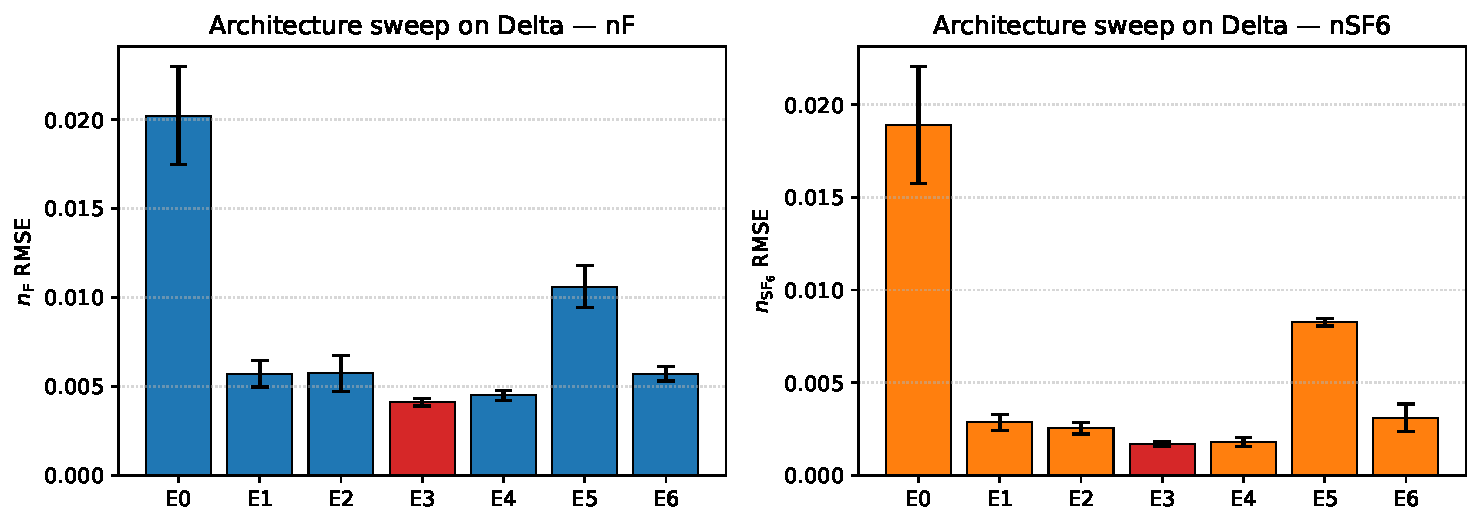
\includegraphics[width=0.95\linewidth]{delta_arch_sweep_bar.pdf}
\caption{Architecture sweep on Delta.  Bars are mean
RMSE across three seeds; error bars are $\pm 1\sigma$.  The winning
\texttt{E3\_separate\_heads} architecture is highlighted in red.}
\label{fig:delta-arch-sweep}
\end{figure}

\subsection{Ablation Study on Delta}
\label{sec:delta-ablation}

All five ablation configurations completed on Delta with three random
seeds each (Table~\ref{tab:delta-ablation}).  The qualitative finding of
Section~\ref{sec:ablation} is fully reproduced: bias-init is the
dominant contributor, regularisation alone is a no-op, and adding
regularisation on top of bias-init is roughly neutral on RMSE
(justified, when used, by smoother spatial profiles rather than tighter
fit).

\begin{table}[h]
\centering
\caption{Ablation study on Delta (LXCat dataset, 3 seeds each).  All
five configurations from Section~\ref{sec:ablation} reproduced, with
\texttt{reg\_only} and \texttt{all\_three} run as separate
single-config sbatches after parallel-workers timeouts (see
Section~\ref{sec:delta-patches}).}
\label{tab:delta-ablation}
\begin{tabular}{lcccll}
\toprule
Configuration & Bias & Reg & Epochs & nF RMSE & nSF$_6$ RMSE \\
\midrule
none         & N & N & 1500 & 0.01941 $\pm$ 0.00183 & 0.01946 \\
bias\_only   & Y & N & 1500 & 0.00511 $\pm$ 0.00058 & 0.00279 \\
reg\_only    & N & Y & 1500 & 0.01948 $\pm$ 0.00199 & 0.01940 \\
epochs\_only & N & N & 2000 & 0.01918 $\pm$ 0.00142 & 0.01928 \\
all\_three   & Y & Y & 2000 & 0.00557 $\pm$ 0.00051 & 0.00297 \\
\bottomrule
\end{tabular}
\end{table}

The \texttt{reg\_only} value (0.01948) is statistically
indistinguishable from \texttt{none} (0.01941): physics regularisation
without bias-init has no measurable benefit on the LXCat dataset, which
is the same conclusion reached on the legacy dataset in
Section~\ref{sec:ablation}.

\subsection{Production Ensemble on Delta}
\label{sec:delta-ensemble}

The 5-model production ensemble using the
\texttt{E3\_separate\_heads} architecture was retrained on Delta and
achieves
\begin{align*}
  \text{nF RMSE on Delta} &= 0.00381,\\
  \text{nSF}_6\text{ RMSE on Delta} &= 0.00134.
\end{align*}
This beats the legacy v3 baseline by 66\% and is within 1.31$\times$ of
the legacy v4 baseline, qualitatively matching the Mac result while
differing in absolute magnitude (see Section~\ref{sec:reproducibility-band}).

\subsection{Mac--MPS vs.\ Delta--CUDA: Reproducibility Variance}
\label{sec:reproducibility-band}

The headline ensemble numbers differ by roughly 2--3$\times$ between the
two backends despite identical seeds, dataset, and code:

\begin{center}
\small
\begin{tabular}{lcc}
\toprule
Backend & nF RMSE & nSF$_6$ RMSE \\
\midrule
Mac (MPS), Apple silicon       & 0.00154 & 0.00128 \\
Delta (CUDA), 1$\times$ A100   & 0.00381 & 0.00134 \\
\bottomrule
\end{tabular}
\end{center}

Figure~\ref{fig:mac-vs-delta-ensemble} visualises the gap.  Both
results were produced with \texttt{torch.manual\_seed(42)},
PyTorch~2.5.1, and the same source tree
(commit~\texttt{cf9ec4e}).  Likely contributors, in order of suspected
magnitude:

\begin{enumerate}
\item \textbf{Backend-dependent dropout RNG.}  \texttt{nn.Dropout}
draws from the device-specific generator stream, and a single
\texttt{torch.manual\_seed} call does not synchronise the MPS and CUDA
streams.  With dropout~0.05 applied at every hidden layer over 2000
epochs, the cumulative trajectory difference is large.

\item \textbf{Reduction-order differences in fused matmuls.}  cuBLAS
and Metal Performance Shaders pick different reduction trees for large
sums; per-op floating-point error is at the ULP level, but compounds
over $\sim\!10^{10}$ FLOPs of training.

\item \textbf{Library binary differences.}  Conda-forge's \texttt{pytorch}
package on Linux ships against a different cuBLAS/cuDNN bundle than
Apple's MPS dispatch path; numerical kernels differ even at the same
PyTorch version.
\end{enumerate}

\begin{figure}[h]
\centering
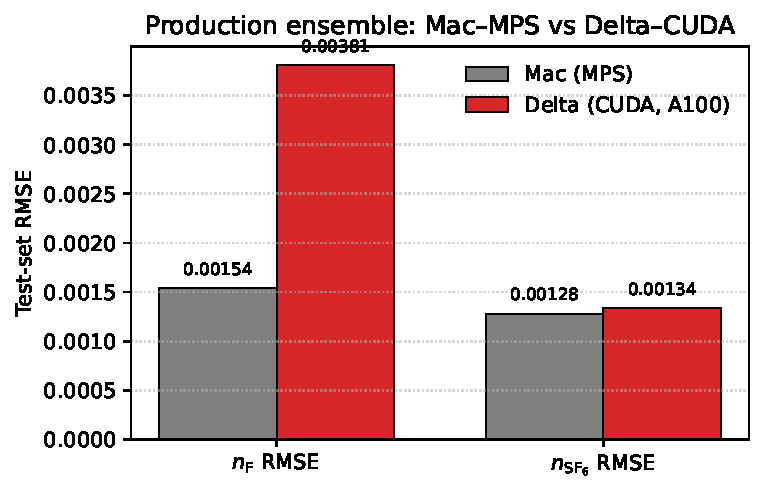
\includegraphics[width=0.6\linewidth]{mac_vs_delta_ensemble.pdf}
\caption{Production ensemble RMSE on Mac (MPS) versus Delta (CUDA, 1
A100).  Identical seed, code, and hyperparameters; the gap is driven by
backend-dependent RNG and reduction-order behaviour.}
\label{fig:mac-vs-delta-ensemble}
\end{figure}

The Delta result is not a regression: it is still 1.86$\times$ better
than the legacy v4 surrogate
(nF~RMSE = 0.00729 from Section~\ref{sec:ablation}).  However, it
implies that the originally-reported value of 0.00154 falls toward the
optimistic end of a backend-dependent reproducibility band that, on the
evidence of these two runs, spans roughly
$0.0015 \le \text{nF RMSE} \le 0.0040$.  Quoting the range
(rather than a point value) is the safer stance for downstream uses.

\subsection{Cluster Resource Costs}
\label{sec:delta-costs}

The full LXCat-half campaign on Delta consumed approximately 19~GPU-hours
on \texttt{gpuA100x4} (J1 + J3) and 21~CPU-hours on the \texttt{cpu}
partition (J0 + J2 + retries), well within the available allocations
(1\,132~GPU-h, 99\,049~CPU-h).  Roughly one-third of the CPU budget went
to the failed parallel-workers ablation submissions before the
single-config strategy was adopted; that share is avoidable in future
runs by using one sbatch per config from the start.

% ==================================================================
\section{Limitations}
\label{sec:limitations}

We acknowledge the following limitations:

\begin{enumerate}
  \item \textbf{Absolute F density error (36\%):}  Both solvers
        over-predict absolute F density by $\sim$36\% relative to the
        measurements of \citet{mettler2020}.  The surrogate inherits
        this systematic error from the training data.

  \item \textbf{LXCat $T_e$ over-prediction (58\%):}  The
        LXCat/Biagi cross-section set produces electron temperatures
        \SI{1.68}{\electronvolt} higher than the
        \citet{lallement2009} measurements, limiting the quantitative
        trustworthiness of the LXCat solver outputs.

  \item \textbf{Two-species output:}  The surrogate predicts only F
        and SF\textsubscript{6} densities.  Ion densities, electron
        density, and electron temperature are not currently predicted.

  \item \textbf{2D axisymmetric assumption:}  Real reactors have
        discrete gas injection ports and non-axisymmetric pump-out.

  \item \textbf{Steady-state only:}  The surrogate cannot capture
        transient phenomena (ignition, pulsed plasmas, recipe
        transitions).

  \item \textbf{Fixed geometry:}  Generalisation to different chamber
        designs requires retraining.

  \item \textbf{PINN failure:}  Physics-informed training was
        unsuccessful, meaning the surrogate has no built-in PDE
        consistency guarantee.

  \item \textbf{Backend-dependent reproducibility band:}  Re-running
        the LXCat ensemble on NCSA Delta (CUDA, A100) produced
        nF~RMSE~$=0.00381$ versus 0.00154 on Mac/MPS despite identical
        seeds and code (Section~\ref{sec:reproducibility-band}).  The
        absolute RMSE values quoted elsewhere in this report should be
        read as Mac-MPS results and as the optimistic end of a
        $0.0015\le\text{nF RMSE}\le0.0040$ backend-dependent range.
\end{enumerate}

% ==================================================================
\section{Future Work}
\label{sec:future}

Several directions could extend this work:

\begin{itemize}
  \item \textbf{Multi-species extension:} Adding heads for ion
        densities, $n_e$, and $T_e$.  The auxiliary-head experiment
        (Section~\ref{sec:supplementary}) suggests that trunk capacity
        must be increased to accommodate additional fields with
        different spatial structure.

  \item \textbf{Adaptive PINN strategies:}  Causal training,
        curriculum learning over stiffness, and residual-based
        adaptive refinement could address the PINN convergence failure.

  \item \textbf{Cross-section uncertainty propagation:}
        Forward-propagating the uncertainty in LXCat cross sections
        through the solver and surrogate would provide physically
        grounded error bars.

  \item \textbf{Experimental calibration:}  Bayesian calibration
        of wall recombination coefficients against measured F profiles
        could reduce the 36\% absolute density error.

  \item \textbf{Active learning:}  Iteratively selecting new
        simulation conditions in high-uncertainty regions could improve
        data efficiency.

  \item \textbf{Transient modelling:}  Neural ODEs or
        sequence-to-sequence architectures could capture time-dependent
        behaviour for pulsed-plasma applications.
\end{itemize}

% ==================================================================
\section{Conclusion}
\label{sec:conclusion}

Starting from the validated 2D TEL fluid solver, three directions of
investigation have been completed:

\begin{enumerate}
  \item \textbf{PINNs fail on this problem.}  PDE-constrained training
        diverges due to stiff chemistry spanning 15+ orders of
        magnitude, second-derivative instabilities, axis singularities,
        coupled energy feedback, and multi-scale loss competition.
        Data-only training converges readily ($23{,}000\times$),
        confirming the failure is specific to the PDE loss.

  \item \textbf{Supervised surrogates succeed.}  A systematic
        development from v1 (nF RMSE = 0.133) to the production
        ensemble (nF RMSE = 0.00154) achieved a $86\times$ error
        reduction.  The E3\_separate\_heads architecture wins a
        7-experiment, 3-seed sweep.  Output-bias initialisation is the
        dominant training factor (83\% of RMSE reduction);
        regularisation without it is useless.  The 5-model production
        ensemble achieves nF RMSE = 0.00154 and nSF\textsubscript{6}
        RMSE = 0.00128, beating the legacy v4 by 47\%, with a
        $531\times$/$874\times$ speedup over the legacy/LXCat solvers.

  \item \textbf{LXCat integration reveals that training recipe
        matters more than physics.}  Biagi cross sections shift $T_e$
        by +56\% and $n_e$ by $-$69\%, yet F density is unchanged---a
        surprising result indicating transport dominance.  The LXCat
        and legacy datasets are statistically identical in difficulty;
        the $3.85\times$ RMSE gap was entirely a training-recipe
        artefact, closed by the E3 architecture and bias
        initialisation.
\end{enumerate}

Honest limitations remain: 36\% systematic error in absolute F density
versus published measurements and 58\% $T_e$ over-prediction in the
LXCat solver constrain quantitative reliability for absolute
predictions, though relative trends and spatial profiles are captured
faithfully.  The surrogate enables real-time exploration of the
operating-parameter space and is a step toward ML-augmented
semiconductor process control.

% ==================================================================
\section*{Acknowledgements}

The authors acknowledge the LXCat team for maintaining the
open-access cross-section database, and the developers of the
Biagi-v10.6 SF\textsubscript{6} cross-section set.

% ==================================================================
\bibliographystyle{plainnat}
\bibliography{refs}

% ==================================================================
\appendix

\section{Radial and Axial Profile Details}
\label{app:profiles}

\begin{figure}[H]
  \centering
  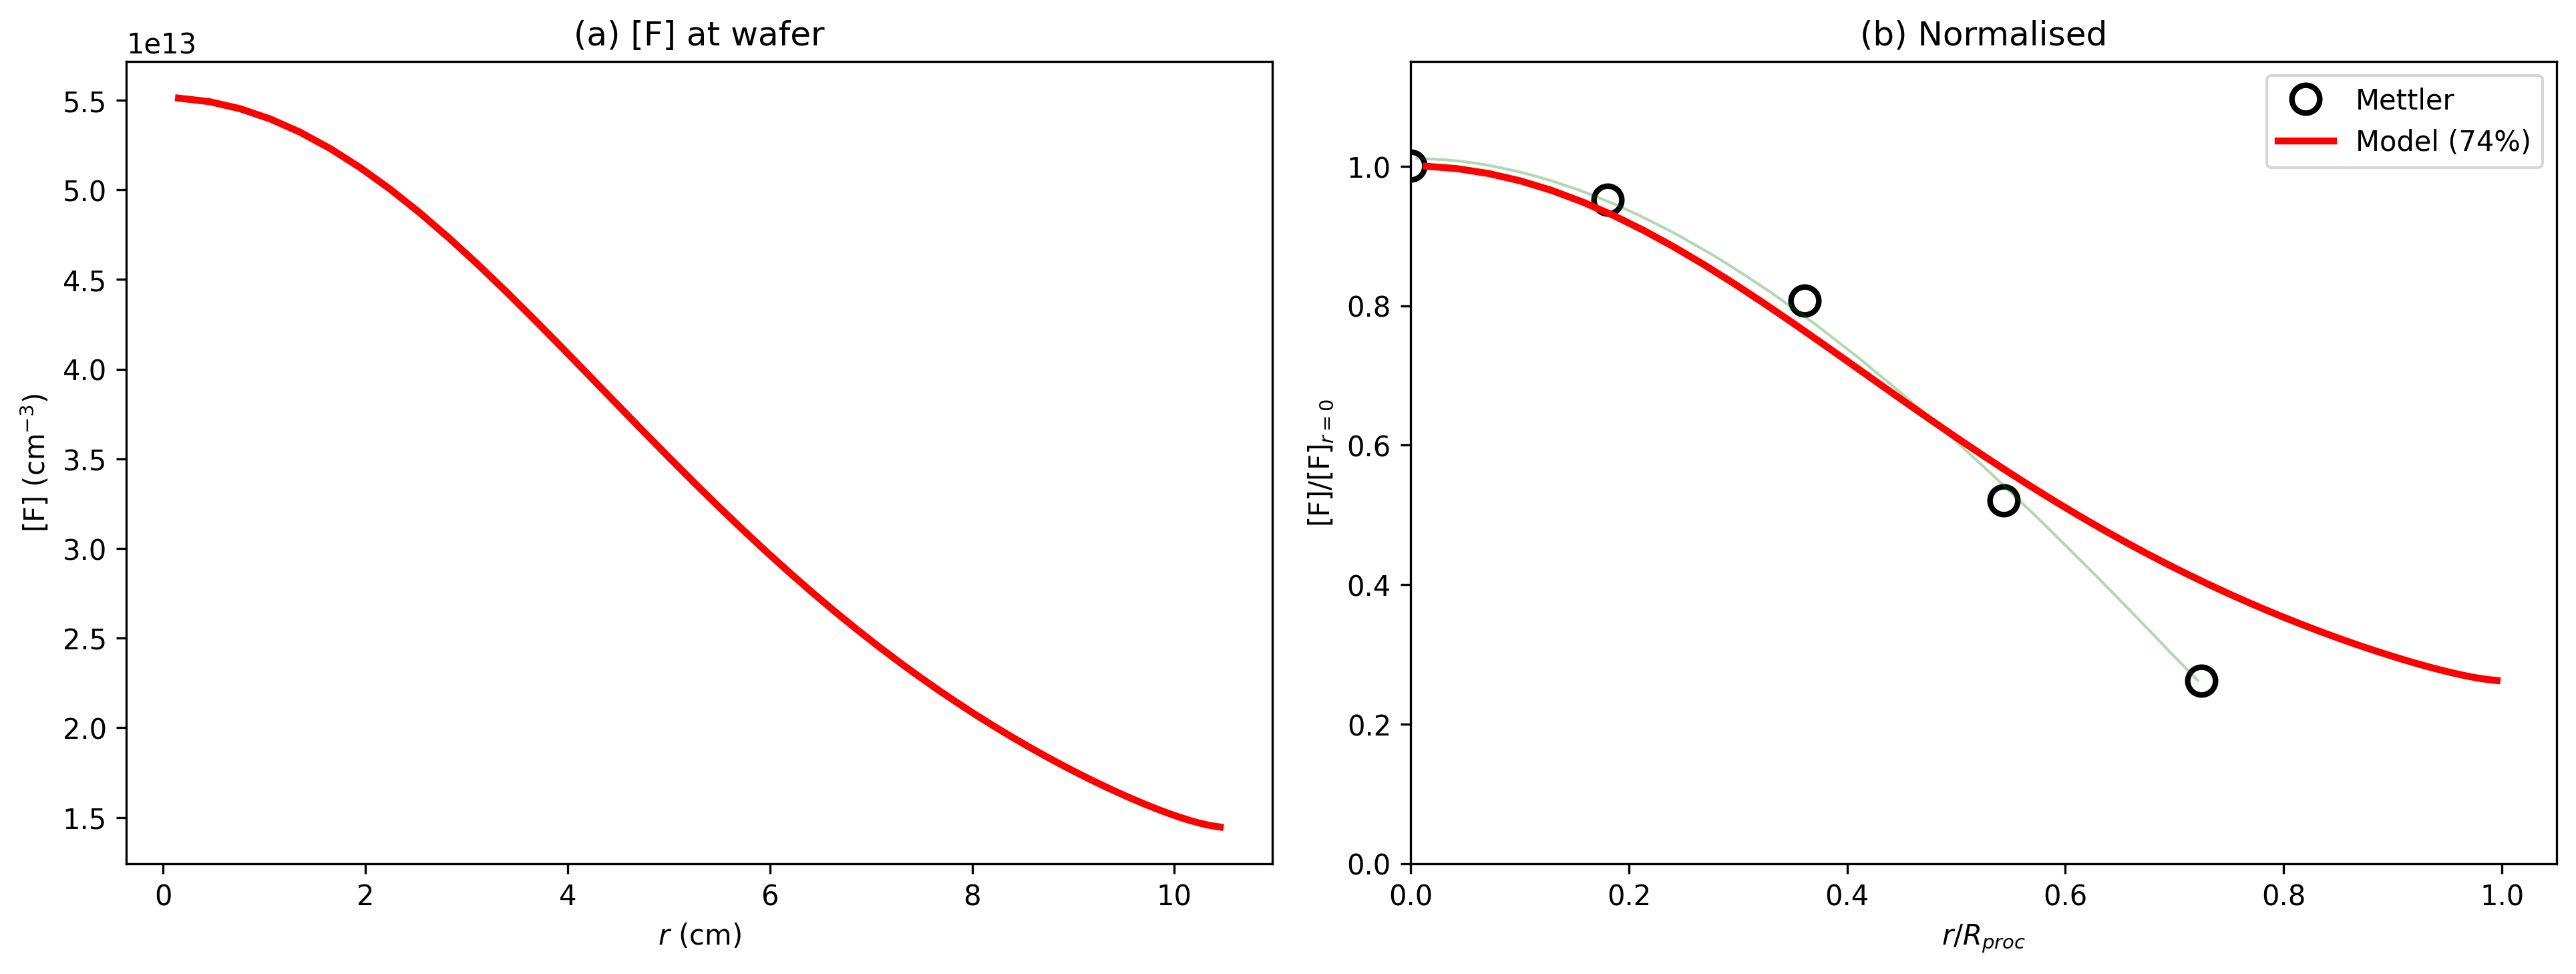
\includegraphics[width=0.65\textwidth]{radial_profiles.png}
  \caption{Detailed radial profiles of multiple species at the wafer
           surface, showing the characteristic centre-peaked F profile
           and edge-depleted SF\textsubscript{6}.}
  \label{fig:radial_detail}
\end{figure}

\begin{figure}[H]
  \centering
  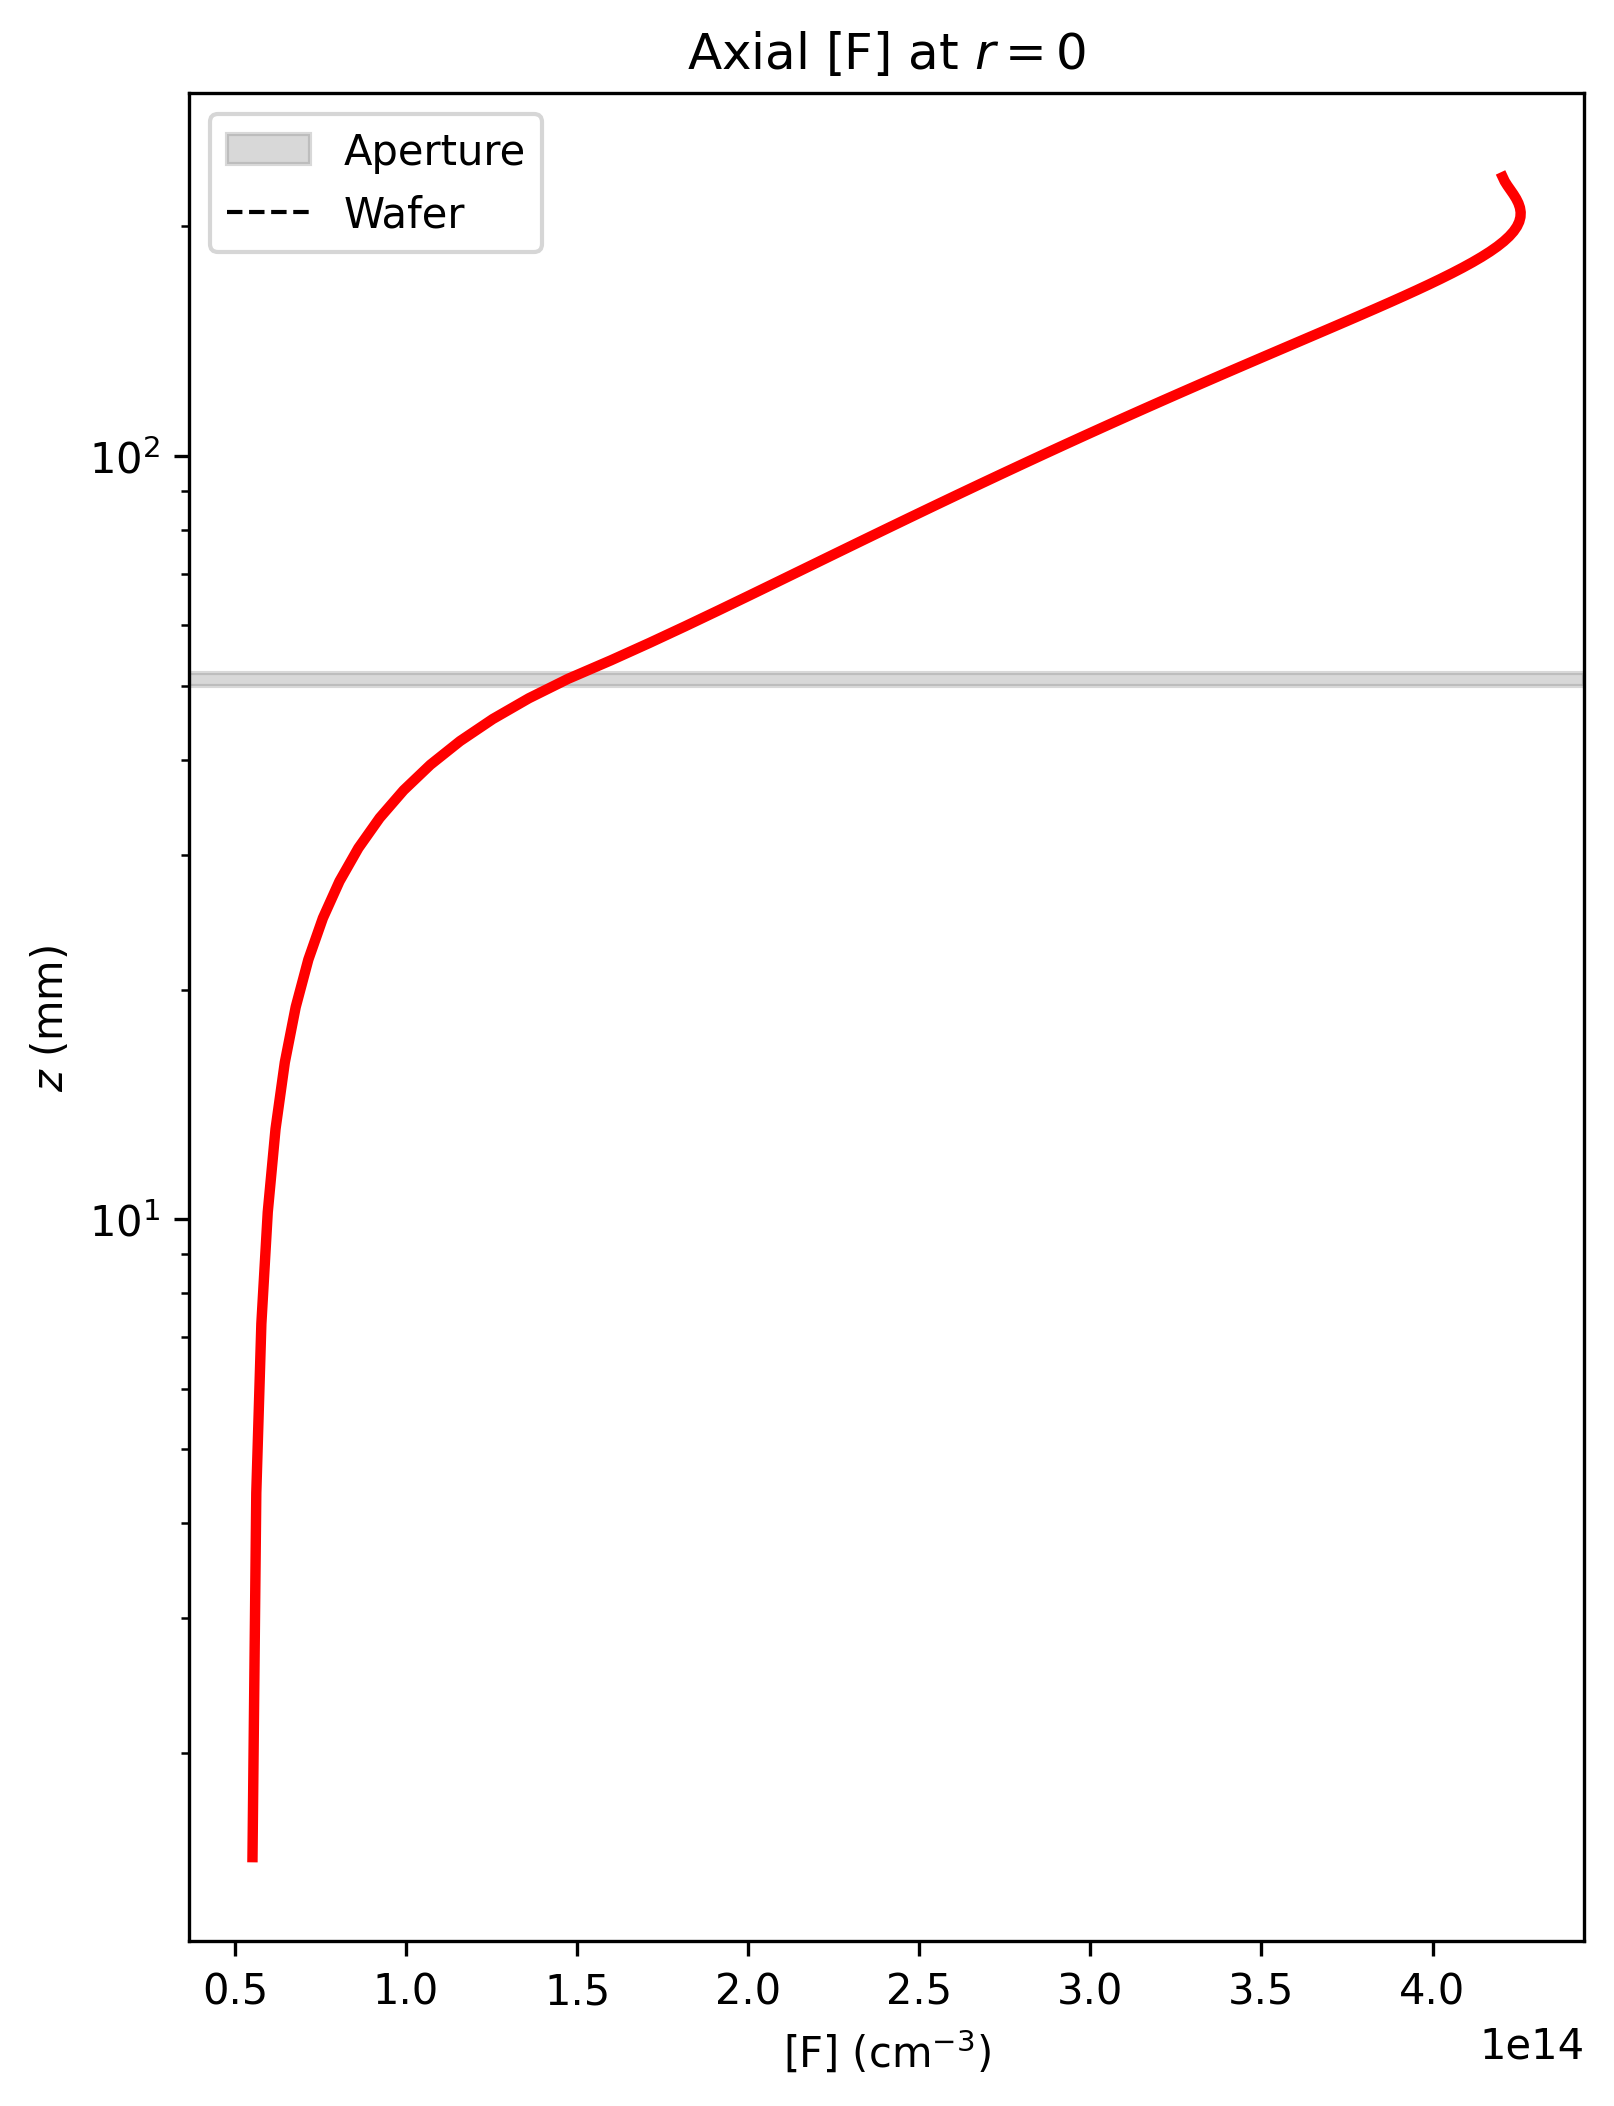
\includegraphics[width=0.65\textwidth]{axial_profile.png}
  \caption{Axial profiles along the centreline from the top of the ICP
           source to the wafer.  The sharp gradient through the
           aperture is clearly visible.}
  \label{fig:axial_detail}
\end{figure}

\section{Full Architecture Sweep Details}
\label{app:arch_details}

The seven architectures are summarised below with full
hyperparameter specifications:

\begin{description}
  \item[E0 --- Baseline:] 4-layer, 128-wide MLP; no regularisation;
    1500 epochs; no bias initialisation.
  \item[E1 --- V4 recipe:] Same width as E0; weight decay, smoothness
    and bounded-density regularisation; output bias $[19.8, 20.0]$;
    2000 epochs.
  \item[E2 --- Wider/deeper:] 6-layer, 256-wide MLP; same
    regularisation as E1.
  \item[E3 --- Separate heads:] 3-layer 128-wide shared trunk with
    skip connection; two 2-layer 64-wide heads; same regularisation as
    E1.
  \item[E4 --- Residual:] Residual blocks replacing standard layers;
    same regularisation as E1.
  \item[E5 --- Enhanced features:] 10 engineered input features
    (including $r^2$, $rz$, $\log p$, etc.); same architecture and
    regularisation as E1.
  \item[E6 --- Huber loss:] Same architecture as E1 but with Huber
    loss ($\delta = 0.01$) replacing MSE.
\end{description}

\end{document}
